%----------------------------------------------------------------------------------------
%	PACKAGES AND OTHER DOCUMENT CONFIGURATIONS
%----------------------------------------------------------------------------------------

\documentclass[
11pt, % The default document font size, options: 10pt, 11pt, 12pt
%oneside, % Two side (alternating margins) for binding by default, uncomment to switch to one side
english, % ngerman for German
singlespacing, % Single line spacing, alternatives: onehalfspacing or doublespacing
%draft, % Uncomment to enable draft mode (no pictures, no links, overfull hboxes indicated)
%nolistspacing, % If the document is onehalfspacing or doublespacing, uncomment this to set spacing in lists to single
%liststotoc, % Uncomment to add the list of figures/tables/etc to the table of contents
%toctotoc, % Uncomment to add the main table of contents to the table of contents
%parskip, % Uncomment to add space between paragraphs
%nohyperref, % Uncomment to not load the hyperref package
headsepline, % Uncomment to get a line under the header
%chapterinoneline, % Uncomment to place the chapter title next to the number on one line
%consistentlayout, % Uncomment to change the layout of the declaration, abstract and acknowledgements pages to match the default layout
]{MastersDoctoralThesis} % The class file specifying the document structure

\usepackage[utf8]{inputenc} % Required for inputting international characters
\usepackage[T1]{fontenc}

%\usepackage{mathpazo} % Use the Palatino font by default
% needs to be turned off for cyrilic

%Russian-specific packages
%--------------------------------------
\usepackage[T2A]{fontenc}
\usepackage[utf8]{inputenc}
\usepackage[russian]{babel}

%\usepackage[backend=bibtex,style=authoryear,natbib=true]{biblatex} % Use the bibtex backend with the authoryear citation style (which resembles APA)

% chicago style but with comma 
\usepackage[style=chicago-authordate,strict,backend=bibtex8, maxcitenames=2, maxbibnames=999%
babel=other,bibencoding=inputenc]{biblatex}
\renewcommand*{\nameyeardelim}{\addcomma\space}

\addbibresource{openbiodiv.bib} % The filename of the bibliography

% long citations

\makeatletter
\newcommand{\tempmaxup}[1]{\def\blx@maxcitenames{\blx@maxbibnames}#1}
\makeatother

\DeclareCiteCommand{\longfullcite}[\tempmaxup]
  {\usebibmacro{prenote}}
  {\usedriver
     {\DeclareNameAlias{sortname}{default}}
     {\thefield{entrytype}}}
  {\multicitedelim}
  {\usebibmacro{postnote}}

\usepackage[autostyle=true]{csquotes} % Required to generate language-dependent quotes in the bibliography

%code listings
\usepackage{listings}
\usepackage{soul} % for underline

\usepackage{algorithm}
\usepackage{algpseudocode}

\lstdefinestyle{customr}{
  belowcaptionskip=1\baselineskip,
  breaklines=true,
 % frame=L,
  xleftmargin=\parindent,
  language=R,
  showstringspaces=false,
  basicstyle=\footnotesize\ttfamily,
  keywordstyle=\bfseries\color{black!40!black},
  commentstyle=\itshape\color{purple!40!black},
  identifierstyle=\color{black},
  stringstyle=\color{black},
}

\lstdefinestyle{customsparql}{
  belowcaptionskip=1\baselineskip,
  breaklines=true,
 % frame=L,
  xleftmargin=\parindent,
  language=SPARQL,
  showstringspaces=false,
  basicstyle=\footnotesize\ttfamily,
  keywordstyle=\bfseries\color{black!40!black},
  commentstyle=\itshape\color{purple!40!black},
  identifierstyle=\color{black},
  stringstyle=\color{black},
}


\newcommand\cl{\lstinline[style=customr]}

\def\todo#1{\medskip\par\noindent\textcolor{red}{\bf TODO: #1}\par\medskip}
\def\KIRIL#1{\medskip\par\noindent\textcolor{red}{\bf KIRIL: #1}\par\medskip}
\def\LYUBO#1{\medskip\par\noindent\textcolor{red}{\bf LYUBO: #1}\par\medskip}

%----------------------------------------------------------------------------------------
%	MARGIN SETTINGS
%----------------------------------------------------------------------------------------

\geometry{
	paper=a4paper, % Change to letterpaper for US letter
	inner=2.5cm, % Inner margin
	outer=3.8cm, % Outer margin
	bindingoffset=.5cm, % Binding offset
	top=1.5cm, % Top margin
	bottom=1.5cm, % Bottom margin
	%showframe, % Uncomment to show how the type block is set on the page
}

%----------------------------------------------------------------------------------------
%	THESIS INFORMATION
%----------------------------------------------------------------------------------------
\thesistitle{OpenBiodiv: отворена система за управление на данни за биологичното разнообразие} % Your thesis title, this is used in the title and abstract, print it elsewhere with \ttitle
\supervisor{проф. д-р Любомир \textsc{Пенев}} % Your supervisor's name, this is used in the title page, print it elsewhere with \supname
\consultant{доц. д-р Кирил \textsc{Симов}}

\examiner{} % Your examiner's name, this is not currently used anywhere in the template, print it elsewhere with \examname
\degree{``доктор''} % Your degree name, this is used in the title page and abstract, print it elsewhere with \degreename
\degreeprogram{``Информатика'' (01.01.2012 г.)}
\profession{4.6 ``Информатика и компютърни науки''}
\author{Виктор \textsc{Сендеров}} % Your name, this is used in the title page and abstract, print it elsewhere with \authorname
\addresses{} % Your address, this is not currently used anywhere in the template, print it elsewhere with \addressname

\subject{Biological Sciences} % Your subject area, this is not currently used anywhere in the template, print it elsewhere with \subjectname
\keywords{} % Keywords for your thesis, this is not currently used anywhere in the template, print it elsewhere with \keywordnames
\university{\href{http://www.bas.bg}{Българска академия на науките}}
\company{\href{http://pensoft.net}{Академично издателство "Пенсофт"}}

% Your university's name and URL, this is used in the title page and abstract, print it elsewhere with \univname
\department{\href{http://www.iict.bas.bg}{Институт по
информационни и комуникационни технологии }} % Your department's name and URL, this is used in the title page and abstract, print it elsewhere with \deptname
\group{\href{http://http://lml.bas.bg/}{Лингвистично моделиране и обработка на знания}} % Your research group's name and URL, this is used in the title page, print it elsewhere with \groupname



\AtBeginDocument{
\hypersetup{pdftitle=\ttitle} % Set the PDF's title to your title
\hypersetup{pdfauthor=\authorname} % Set the PDF's author to your name
\hypersetup{pdfkeywords=\keywordnames} % Set the PDF's keywords to your keywords
}

\begin{document}

\frontmatter % Use roman page numbering style (i, ii, iii, iv...) for the pre-content pages

\pagestyle{plain} % Default to the plain heading style until the thesis style is called for the body content

%----------------------------------------------------------------------------------------
%	TITLE PAGE
%----------------------------------------------------------------------------------------

\begin{titlepage}
\begin{center}
\vspace*{.06\textheight}
{\scshape\LARGE \univname\par}\vspace{1.5cm} % University name
{\scshape\LARGE \compname\par}\vspace{1.5cm} % University name
\textsc{\Large АВТОРЕФЕРАТ}\\[0.5cm] % Thesis type

\HRule \\[0.4cm] % Horizontal line
{\huge \bfseries \ttitle\par}\vspace{0.4cm} % Thesis title
\HRule \\[1.5cm] % Horizontal line
 
\begin{minipage}[t]{0.4\textwidth}
\begin{flushleft} \large
\emph{Автор:}\\
\href{http://senderov.net}{\authorname} % Author name - remove the \href bracket to remove the link
\end{flushleft}
\end{minipage}
\begin{minipage}[t]{0.4\textwidth}
\begin{flushright} \large
\emph{Научен ръководител:} \\
\href{http://pensoft.net}{\supname} \\ % Supervisor name - remove the \href bracket to remove the link  
\emph{Научен консултант:} \\
\href{http://bultreebank.org/en/our-team/kiril-simov/}{\consname} % Supervisor name - remove the \href bracket to remove the link  

\end{flushright}
\end{minipage}\\[3cm]

% TODO Ask Kiril about научна област, научна специалност от заглавната страница на автореферата
\large 
\textit{За придобиване на образователната и научна степен \degreename\\
по докторска програма \degreeprogramname\\
професионално направление \professionname}\\[0.3cm] % University requirement text

\vfill

%{\large \today}\\[4cm] % Date
%\includegraphics{Logo} % University/department logo - uncomment to place it
 
\vfill
\end{center}
\end{titlepage}

%----------------------------------------------------------------------------------------
%	DECLARATION PAGE
%----------------------------------------------------------------------------------------

% \begin{declaration}
% \addchaptertocentry{\authorshipname} % Add the declaration to the table of contents
% \noindent I, \authorname, declare that this thesis titled, \enquote{\ttitle} and the work presented in it are my own. I confirm that:

% \begin{itemize} 
% \item This work was done wholly or mainly while in candidature for a research degree at this University.
% \item Where any part of this thesis has previously been submitted for a degree or any other qualification at this University or any other institution, this has been clearly stated.
% \item Where I have consulted the published work of others, this is always clearly attributed.
% \item Where I have quoted from the work of others, the source is always given. With the exception of such quotations, this thesis is entirely my own work.
% \item I have acknowledged all main sources of help.
% \item Where the thesis is based on work done by myself jointly with others, I have made clear exactly what was done by others and what I have contributed myself.\\
% \end{itemize}
 
% \noindent Signed:\\
% \rule[0.5em]{25em}{0.5pt} % This prints a line for the signature
 
% \noindent Date:\\
% \rule[0.5em]{25em}{0.5pt} % This prints a line to write the date
% \end{declaration}

% \cleardoublepage




\mainmatter % Begin numeric (1,2,3...) page numbering

\pagestyle{thesis} % Return the page headers back to the "thesis" style

% Chapter 1
\addchap{Introduction}
\label{chapter-introduction} 
%----------------------------------------------------------------------------------------
% Define some commands to keep the formatting separated from the content 
\newcommand{\keyword}[1]{\textbf{#1}}
\newcommand{\tabhead}[1]{\textbf{#1}}
\newcommand{\code}[1]{\texttt{#1}}
\newcommand{\file}[1]{\texttt{\bfseries#1}}
\newcommand{\option}[1]{\texttt{\itshape#1}}
%----------------------------------------------------------------------------------------
\section*{Importance of the topic}
\addcontentsline{toc}{section}{Importance of the topic}  
The desire for an integrated information system serving the needs of the biodiversity community dates at least as far back as 1985 when the Taxonomy Database Working Group (TDWG)---later renamed to Biodiversity Informatics Standards but retaining the abbreviation TDWG---was established\footnote{A webpage with the history of TDWG dating back to 1985 can be viewed under \url{http://old.tdwg.org/past-meetings/}; however, a lot of the links are unfortunately broken and the page needs some maintenance.}. In 1999, the Global Biodiversity Information Facility (GBIF) was created after the Organization for Economic Cooperation and Development (OECD) had arrived at the conclusion that ``an international mechanism is needed to make biodiversity data and information accessible worldwide'' (\cite{noauthor_what_nodate}).  The Bouchout declaration (\cite{noauthor_bouchout_2014}) crowned the results of the European Union--funded project \cite{noauthor_pro-ibiosphere_nodate} that lasted from 2012 to 2014 and was dedicated to the task of creating an integrated biodiversity information system. The Bouchout declaration proposes to make scholarly biodiversity knowledge freely available as Linked Open Data (LOD).  A parallel process in the U.S.A. started even earlier with the establishment of the Global Names Architecture, GNA (\cite{patterson_names_2010,pyle_towards_2016}).

In 2014, the Horizon 2020 BIG4 consortium was formed between academia and industry dedicated to advancing biodiversity science.  The project's mission statement reads ``BIG4---Biosystematics, Informatics and Genetics of the big 4 insect groups: training tomorrow's researchers and entrepreneurs'' (\cite{university_of_copenhagen_big4_2014}). An important member of the consortium is the academic publishing house and software company, Pensoft Publishers. Pensoft publishes several dozen well-known open access taxonomic journals\footnote{For example, ZooKeys, PhytoKeys, MycoKeys, and Biodiversity Data Journal (BDJ).} and, as a signatory of the Bouchout declaration, was a prime candidate to push the vision for an Open Biodiversity Knowledge Management System (OBKMS) forward. The presented Ph.D. project is based at Pensoft Publishers and at the Institute of Information and Communication Technology (IICT) of the Bulgarian Academy of Sciences with the goal to follow through pro-iBiosphere's vision.

\section*{Previous work}
\addcontentsline{toc}{section}{Previous work}

Due to the interdisciplinary nature of the thesis, this section will focus on two areas: (a) knowledge bases and Linked Open Data and (b) biodiversity publishing.

\subsection*{Knowledge bases and Linked Open Data}
\addcontentsline{toc}{subsection}{Knowledge bases and Linked Open Data}

We shall start by first introducing \emph{knowledge bases} and \emph{knowledge-based systems}.  We use the two terms interchangeably but tend to write the longer variant, knowledge-based system, when we want to emphasize aspects of the knowledge base that are not related to the underlying facts store (database).

It is useful to form one's concept of knowledge-based systems both by looking at explicit definitions and by looking at several examples of knowledge bases in practice. The term was already being widely discussed by the 1980's (\cite{brodie_kbms_1989}) and early nineties (\cite{harris_knowledge_1993}) and was understood to mean the utilization of ideas from both database management systems (DBMS) and artificial intelligence (AI) to create a type of computer system called \emph{knowledge base management system} (KBMS). \cite{harris_knowledge_1993} writes that the characteristics of a knowledge base management system are that it contains ``prestored rules and facts from which useful inferences and conclusions may be drawn by an inference engine.''  We should note that the phrase ``prestored rules'' comes from the time of first-generation AI systems that were rule-based. Recently, there has been progress in incorporating statistical techniques into databases (\cite{mansinghka_bayesdb:_2015}); however, in this project we are working with the classical rule-based definition. In other words, a knowledge base is, in our understanding, a suitable database tightly integrated with a logic layer.

Another relatively more recent development in knowledge-based systems has been the application of the Linked Data principles (\cite{heath_linked_2011}). In fact, most existing knowledge bases emphasize the community aspects of making data more interconnected and reusable. Examples include Freebase (\cite{bollacker_freebase:_2008}), which was recently incorporated in WikiData (\cite{vrandecic_wikidata:_2014, pellissier_tanon_freebase_2016}), DBPedia (\cite{hutchison_dbpedia:_2007}), as well as Wolfram|Alpha (\cite{noauthor_wolfram|alpha_nodate}) and the Google Knowledge Graph (\cite{singhal_introducing_2012}). What these systems have in common is that an emphasis is placed not only on the logic layer allowing inference but on a unified information space: these systems act as nexus integrating information from multiple places and they follow to various degrees the principles of Linked Open Data (LOD).

Linked Open Data (\cite{heath_linked_2011}) is a concept of the Semantic Web (\cite{berners-lee_semantic_2001}), which, when applied properly, ensures that data published on the Web is reusable, discoverable, and most importantly ensures that pieces of data published by different entities can work together.  We will discuss the Linked Data principles and their application to OpenBiodiv in detail in Chapter~\ref{chapter-lod}.

Leveraging these developments modern knowledge bases place a bigger emphasis on interlinking data rather than on developing a complex inference machinery. There has been critique of the idea of bundling logic in the database layer as such bundling leads to increased complexity (\cite{barrasa_rdf_2017}). The critique can be summarized with two points. First, bundling the logic near the data (especially when it is excessive for the task at hand) can lead to drastic performance decreases\footnote{ We will compare the performance of the stronger Web Ontology Language (OWL) logic layer with a weaker RDF Schema (RDFS) logic layer in Chapter~\ref{chapter-lod}. Resource Description Format (RDF) is a data model for storing statements about things discussed later.}. Second, the developing of new techniques (e.g. machine learning) can make the existing deep logic layer obsolete. Our view is that data is the commodity which is much more valuable, and the inference strategy (be it a rule-based logic layer, or a statistical machine learning technique) can be replaced as computational science moves forward. These ideas lead to an interesting conundrum in the choice of a database technology discussed in the subsequent sections.

Finally, a knowledge-based system ultimately needs to include user-interface components (UI's) and application programming interfaces (API's) or an application layer. These serve as the point-of-contact between human and machine, or machine and machine and are crucial to the success of any such system.

\subsection*{Biodiversity publishing}
\addcontentsline{toc}{subsection}{Biodiversity publishing}

In the biomedical domain there are well-established efforts to extract information and discover knowledge from literature (e.g. \cite{rebholz-schuhmann_facts_2005, momtchev_expanding_2009, williams_open_2012}).  The biodiversity domain, and in particular biological systematics and taxonomy (from here on in this thesis referred to as \emph{taxonomy}), is also moving in the direction of semantization of its research outputs (\cite{agosti_biodiversity_2006, patterson_taxonomic_2006,kennedy_scientific_2005,penev_fast_2010, tzitzikas_integrating_2013}).  The publishing domain has been modeled through the Semantic Publishing and Referencing Ontologies, SPAR Ontologies (\cite{peroni_semantic_2014}).   The SPAR Ontologies are a collection of ontologies incorporating, amongst others, FaBiO, the FRBR-aligned Bibliographic Ontology (\cite{peroni_fabio_2012}), and DoCO, the Document Component Ontology (\cite{constantin_document_2016}).   The SPAR Ontologies provide a set of classes and properties for the description of general-purpose journal articles, their components, and related publishing resources.  Taxonomic articles and their components, on the other hand, have been modeled through the TaxPub XML Document Type Definition (DTD)---also referred to loosely as XML schema---and the Treatment Ontologies (\cite{catapano_taxpub:_2010}).  While TaxPub is the XML-schema of taxonomic publishing for several important taxonomic journals (e.g. ZooKeys, PhytoKeys, Biodiversity Data Journal), the Treatment Ontologies are still in development and have served as a conceptual template for OpenBiodiv-O (discussed in Chapter~\ref{chapter-ontology}). 

Taxonomic nomenclature is a discipline with a very long tradition.  It transitioned to its modern form with the publication of the Linnaean System (\cite{linnaeus_systema_1758}).  Already by the beginning of the last century, there were hundreds of taxonomic terms in usage (\cite{witteveen_naming_2015}).  At present the naming of organismal groups is governed by by the International Code of Zoological Nomenclature, ICZN (\cite{international_commission_on_zoological_nomenclature_international_1999}) and by the International Code of Nomenclature for algae, fungi, and plants, Melbourne Code (\cite{mcneill_international_2012}).  Due to their complexity (e.g. ICZN has 18 chapters and 3 appendices), it proved challenging to create a top-down ontology of biological nomenclature. Example attempts include the relatively complete NOMEN ontology (\cite{dmitriev_nomen_2017}) and the somewhat less complete Taxonomic Nomenclatural Status Terms, TNSS\footnote{Even though it is unknown to the authors whether TNSS was published in peer-reviewed literature, remnants of it can still be found on GitHub, e.g. under \url{https://github.com/pensoft/OpenBiodiv/blob/master/ontology/contrib/taxonomic_nomenclatural_status_terms.owl}.}.

There are several projects that are aimed at modeling the broader biodiversity domain conceptually. Darwin Semantic Web, Darwin-SW (\cite{baskauf_darwin-sw:_2016}) adapts the previously existing Darwin Core (DwC) terms (\cite{wieczorek_darwin_2012}) as Resource Description Framework (RDF). These models deal primarily with organismal occurrence data.

Modeling and formalization of the strictly taxonomic domain has been discussed by Berendsohn (\cite{berendsohn_concept_1995}) and later, e.g., in (\cite{franz_perspectives:_2009,sterner_taxonomy_2017}). Noteworthy efforts are the XML-based Taxonomic Concept Transfer Schema (\cite{taxonomic_names_and_concepts_interest_group_taxonomic_2006}) and a now defunct Taxon Concept ontology. Very recently, the TDWG community has attempted to resurrect the Taxon Concept ontology with the Taxonomic Names and Concepts Interest Group. The group discussions can be accessed under \url{https://github.com/tdwg/tnc}. Interestingly the \href{https://github.com/tdwg/tnc/issues/1}{very first GitHub issue} discussed OpenBiodiv-O and the possibility of its adoption as a TDWG standard.

By the time the OpenBiodiv project started in June 2015, a number of articles had been previously published on the topics of linking data and sharing identifiers in the biodiversity knowledge space (\cite{page_biodiversity_2008}), unifying phylogenetic knowledge (\cite{parr_evolutionary_2012}), taxonomic names and their relation to the Semantic Web (\cite{page_taxonomic_2006,patterson_names_2010}), and aggregating and tagging biodiversity research (\cite{mindell_aggregating_2011}). Some partial discussion of OBKMS was to be found in the science blog \href{http://iphylo.blogspot.bg}{iPhylo} (\cite{page_vision_2014, page_putting_2015}). The legal aspects of the OBKMS had been discussed by \cite{egloff_open_2014}.

Furthermore, several tools and systems that deal with the integration of biodiversity and biodiversity data had been developed by different groups. Some of the most important ones are UBio, Global Names, BioGuid, BioNames, Pensoft Taxon Profile, and the Plazi Treatment Repository\footnote{UBio: \href{http://ubio.org/}{http://ubio.org/}; Global Names: \href{http://globalnames.org/}{http://globalnames.org/}; BioGuid: \href{http://bioguid.org/}{http://bioguid.org/}; BioNames: \href{http://bionames.org/}{http://bionames.org/}; Pensoft Taxon Profile: \href{http://ptp.pensoft.eu/}{http://ptp.pensoft.eu/}; Plazi Treatment Repository: \href{http://plazi.org/wiki/}{http://plazi.org/wiki/}.}.

\subsection*{Key findings}
\addcontentsline{toc}{subsection}{Key findings}

The key findings from the papers cited in the previous paragraphs can be summarized as follows:

\begin{enumerate}
  
\item{Biodiversity science deals with disparate types of data: taxonomic, biogeographic, phylogenetic, visual, descriptive, and others. These data are siloed in unlinked data repositories.}
  
\item{Biodiversity databases need a universal system of naming concepts due to the inefficiencies of Linnaean names for modern taxonomy. Taxonomic concept labels have been proposed as a human-readable solution and stable globally unique identifiers of taxonomic concepts had been proposed as a machine-readable solution.}

\item{There is a base of digitized semi-structured biodiversity information online with appropriate licenses waiting to be integrated as a knowledge base.}
\end{enumerate}


\section*{Goal and objectives}
\addcontentsline{toc}{section}{Goal and objectives}

Given the huge international interest in OBKMS, this dissertation started the OpenBiodiv project, the goal of which is to contribute to OBKMS by creating an \ul{open knowledge-based system of biodiversity information extracted from scholarly literature}. In order to complete the system, the following objectives need to be achieved:

\paragraph{Objective 1: Architecture.} Formally define OpenBiodiv as a knowledge-based system and create its integrated software architecture.
\paragraph{Objective 2: Ontology.} Study the domain of biodiversity informatics and biodiversity publishing and develop an ontology allowing data integration from diverse sources.
\paragraph{Objective 3: Linked open dataset.} Create a Linked Open Dataset (LOD) on the basis of published taxonomic articles using the ontology defined in Objective 2.
\paragraph{Objective 4: Library.} Develop methods for converting taxonomic publications into the semantic model of the ontology in order to support Objective 3.
\paragraph{Objective 5: Workflows.} Develop practical workflows for continuously converting taxonomic data into taxonomic publications and thus updating the LOD dataset.
\paragraph{Objective 6: Web portal.} Create a web-portal and example applications on top of the knowledge base.

\section*{Methodology}
\addcontentsline{toc}{section}{Methodology}

This dissertation has a methods and tools orientation: i.e. its goal is not the testing of particular scientific hypothesis but rather the theoretical design and practical implementation of a knowledge-management system. In this section I shall outline the "meta-choices" that I have made---such as what programming and database paradigms to use---before the design and implementation phase. 

\subsection*{Choice of database paradigm for OpenBiodiv}
\addcontentsline{toc}{subsection}{Choice of database paradigm for OpenBiodiv}

We specify OpenBiodiv as a knowledge-based system with a focus on structuring and interlinking biodiversity data. Two of the possible database technologies that fit this requirement are semantic graph databases (triple stores) such as GraphDB (\cite{ontotext_graphdb_2018}) and labeled property graphs such as Neo4J (\cite{neo4j_developers_neo4j_2012}).  Semantic graph databases offer a very simple data model: every fact stored in such a database is composed as a triple of \emph{subject}, \emph{predicate}, and \emph{object}. Subjects of triples are always resource identifiers, whereas objects can be other resource identifiers or literal values (e.g. strings, numbers, etc.).  Links between resources or between resources and literals are given by the predicates (also specified as identifiers). These links are sometimes referred to as \emph{properties}. Thus, one can visualize a graph whose vertices are the objects or subjects given by resource identifiers or literals and whose edges are predicates.

Semantic graph databases have the unique feature that the logic layer is also expressed as triples stored in the database. This logic layer, known as \emph{ontology}, is not only responsible for drawing conclusions from the data (inference), but also specifies the semantics of how knowledge should be expressed.

Labeled property graphs, on the other hand, offer a freer data model by allowing the edges of the knowledge graph to have properties as well. For example, in a labeled property graph whose vertices are two cities A and B and are connected by a property-predicate \emph{connected by road}, it is possible to additionally attach the value ``500 km'' to that property. Thus, we indicate that the length of the road connecting the cities is 500 km.

Note that labeled property graphs are not any more expressive than what can be achieved by triples alone. In fact, complex relationships in a simple triple store can be expressed by making relationships into nodes that have properties on their own. This process is known as \emph{reification}. For example, the two cities $A$ and $B$ can connect to a further vertex, $R$ indicating the road. $R$ will then have three properties: \emph{start}, \emph{end}, and \emph{length}. The value (object) of \emph{start} will be $A$, of \emph{end} will be $B$, and of length will be the literal ``500 km.''

We have summarized the differences between labeled property graphs and semantic graph databases in Table~\ref{graphdb-vs-neo4k}. After careful considerations, we settled on the triple store, i.e. semantic graph database as a choice of database technology. This decision was informed by the wide availability of high-quality ontologies and Resource Description Framework (RDF) data models in our domain (\cite{baskauf_darwin-sw:_2016,peroni_semantic_2014}) and the popularity of the Semantic Web (\cite{berners-lee_semantic_2001}) in the community. Furthermore, our base at a publisher was more suited to a standards-driven foundational project as opposed to a particular application.

\begin{table}
\caption{Differences between semantic graph databases (e.g. GraphDB) and labeled property graphs (e.g. Neo4j).}
\begin{tabular}{>{\centering\arraybackslash}m{2.5cm}|>{\centering\arraybackslash}m{4.2cm}|>{\centering\arraybackslash}m{4.2cm}}
Criterion   & Semantic database & Labeled property graph\\
\hline
Semantics   & Stored in the database itself as OWL or RDFS statements. Provides a uniform data space. Requires expert ontologists to extract knowledge.
            & Formal semantics usually are missing. Quick deployment. Uniform data space harder to achieve.\\
\hline
Inference   & Provided by the database itself from its ontology or expressed as SPARQL queries. General purpose, slower.
            & External to the database. Needs to be written for every specific task. Special purpose. Faster.\\
\hline
Community   & Has a rich and mature community of ontologists and knowledge engineers. Lots of domain ontologies. Designed for inter-operability. Standards-driven.
            & Data models are created ad-hoc by data scientists or programmers for a particular task. Inter-operability requires effort and not of primary concern. Applications-driven.\\
\hline
\end{tabular}
\label{graphdb-vs-neo4k}
\end{table}

However, we believe that labeled property graphs are a freer and a more natural data model and are perfectly suited for biodiversity informatics. In particular they provide a much more natural formalism for relationships between taxonomic concepts (discussed in Chapter~\ref{chapter-ontology}). Also, non-RDF semantic databases such as \mbox{WikiData} are gaining in popularity. Therefore, we believe that the applicability of RDF triple stores for OpenBiodiv should constantly be re\"evaluated.

\subsection*{Choice of information sources}
\addcontentsline{toc}{subsection}{Choice of information sources}

According to \cite{noauthor_pro-ibiosphere_2014}, biodiversity and biodiversity-related data have two different ``life-cycles.'' In the past, after an observation of a living organism had been made, it was recorded on paper and then the observation record was published in paper-based form. In order for biodiversity data to be available to the modern scientist, efforts are made nowadays to digitize those paper-based publications by Plazi \cite{agosti_why_2007} and the Biodiversity Heritage Library (\cite{miller_taxonomic_2012}). For this purpose, several dedicated XML schemas have been developed (see \cite{penev_xml_2011} for a review), of which TaxPub (\cite{catapano_taxpub:_2010}) and TaxonX  seem to be the most widely used (\cite{penev_implementation_2012}). The digitization of publications contains several steps. After scanning and optical character recognition (OCR), text mining is combined with searching for particular kinds of data. This procedure leaves a trace in the form of marked-up (tagged) elements that can then be extracted and made available for future use and reuse (\cite{miller_integrating_2015}).

In present day, biodiversity data and publications are mostly ``born digital'' as semantically Enhanced Publications (EP's, \cite{claerbout_electronic_1992,godtsenhoven_van_emerging_2009,shotton_semantic_2009}). According to \cite{claerbout_electronic_1992}, ``an EP is a publication that is enhanced with research data, extra materials, post publication data and database records. It has an object-based structure with explicit links between the objects. An object can be (part of) an article, a data set, an image, a movie, a comment, a module or a link to information in a database.'' Semantically enhanced publications are thus natives of the Web and the Semantic Web unlike their paper-based predecessors.

The act of publishing in a digital, enhanced format, differs from the ground up from a paper-based publication. The main difference is that a digitally-published document can be structured in such a format as to be suitable both for machine processing and to the human eye. In the sphere of biodiversity science, Pensoft journals such as ZooKeys, PhytoKeys, and the Biodiversity Data Journal (BDJ) already function by providing EP's (\cite{penev_semantic_2010}).

Given the fact that Pensoft Publishers' and Plazi's publications cover a large part of taxonomic literature both in volume and also in temporal span, and the fact that the publications of those two publishers are available as semantic EP's, we've chosen Pensoft's journals and Plazi's treatments as our main sources of information.

Furthermore, we incorporate the taxonomic backbone of GBIF \cite{gbif_secretariat_gbif_2017} as a source for data integration. This is further discussed in Chapter~\ref{chapter-lod}.

\subsection*{Choice of development methodology and programming environment}
\addcontentsline{toc}{subsection}{Choice of development methodology and programming environment}

In 2016, based on the outcomes of pro-iBiosphere and on the previous work in the area of biodiversity informatics, we published the Ph.D. plan for this research (\cite{senderov_open_2016}). This publication can be considered as the first design specification of OpenBiodiv. However, in the course of developing the system, its design was changed iteratively through a feedback loop from collaborators from the \href{http://big4-project.eu}{BIG4 project}\footnote{The Ph.D. candidate, Viktor Senderov, is part of the Marie Skłodowska-Curie BIG4 International Training Network: Biosystematics, informatics and genomics of the big 4 insect groups: training tomorrow's researchers and entrepreneurs.} and various international collaborators. We view this positively and in the spirit of both \emph{open science} and \emph{agile software development} (\cite{beck_manifesto_2001}). This iterative approach differs from the waterfall approach where after a through design phase, the specifications "are frozen" and a lengthy implementation phase.

In recent years, the R programming language has been used widely in the field of data science (\cite{r_core_team_r:_2016}). R has a rich library of software packages including such for processing XML (\cite{wickham_xml2:_2018}), for accessing rest API's (\cite{wickham_httr:_2017}), and focuses on open science (\cite{boettiger_building_2015}). The capabilities of R as function-oriented and interpreted language allow the iterative software development approach outlined in the previous paragraph to proceed rapidly. Furthermore, R is widely adopted in the biodiversity informatics community. For this reason, the R software environment was chosen as the main programming environment.

\subsection*{Open Science and The Semantic Web}
\addcontentsline{toc}{subsection}{Open Science and The Semantic Web}

After having specified the desired design and given the programming language, R, I would like to discuss some methodologies and frameworks that have been adopted to be more efficient, open, and reproducible.

I believe that OpenBiodiv needs to be addressed from the point of view of \emph{Open Science}. According to \cite{kraker_case_2011} and to \cite{noauthor_was_nodate}, the six principles of open science are: open methodology, open source, open data, open access, open peer review, and open educational resources. It is my belief that the aim of open science is to ensure access to the whole research product: data, discoveries, hypotheses, and so on. This opening-up will ensure that the scientific product is reproducible and verifiable by other scientists (\cite{mietchen_transformative_2014}). There is a very high interest in development of processes and instruments enabling reproducibility and verifiability, as can be evidenced for example by a special issue in Nature dedicated to reproducible research (\cite{noauthor_challenges_2010}). Therefore, the source code, data, and publications of OpenBiodiv will be published openly.

Moreover, OpenBiodiv should be thought of as integral part of the Semantic Web (\cite{berners-lee_semantic_2001}). The Semantic Web is a vision for the future of the web where not only documents but also data are connected.

\section*{Structure of the thesis}
\addcontentsline{toc}{section}{Structure of the thesis}

So far the raison d'\^etre of the system and this thesis and an outline of its goal and objectives have been given in this Introduction.
In Chapter~\ref{chapter-openbiodiv}, a formal specification and design of the desired system as well as an outline of its architecture will be presented; this chapter forms Objective 1. The subsequent chapters discuss the implementation of OpenBiodiv. Chapter~\ref{chapter-ontology} gives a conceptualization of the domain of scientific taxonomic publishing formalizes it by introducing the central result of this thesis, the оntology of OpenBiodiv (OpenBiodiv-O) and thus forms Objective 2. Chapter~\ref{chapter-lod} describes the Linked Open Dataset that has been generated based on OpenBiodiv-O and forms Objective 3. Chapter~\ref{chapter-rdf4r} describes in detail the RDF4R software package (an R package for working with RDF), which was used to create the Linked Open Data (OpenBiodiv-LOD) and forms Objective 4. In Chapter~\ref{chapter-case-study}, two case-studies for importing data into OpenBiodiv from important international repositories are discussed and thus it forms Objective 5. Chapter~\ref{chapter-webportal} discusses the website that has being prepared to serve on top of OpenBiodiv-LOD and its applications (Objective 6).
In the Conclusion, I will explain how the results have been published and summarize the main results.


%----------------------------------------------------------------------------------------




\chapter*{Conclusion}
\addcontentsline{toc}{chapter}{Conclusion}
\label{chapter:summary}

\section*{Results}
\addcontentsline{toc}{section}{Results}

We believe that the presented scientific work fulfills the stated objective and tasks. In this section, we will summarize the results achieved and how they relate to the fulfillment of the stated objectives and tasks. In the course of the study all six tasks were achieved and the results were published in prestigious international journals and presented at major conferences in Bulgaria and abroad. The most important results of the thesis are summarized as follows:

\paragraph{Result 1.} The cenral result of the thesis is the creation of a domain conceptualization of biodiversity publishing and a formal ontology OpenBiodiv-O enabling the linking of biodiversity knowledge on the basis of scholarly publications. OpenBiodiv-O serves as the basis of the Linked Open Data OpenBiodiv-LOD. By developing an ontology focusing on biological taxonomy, we provided an ontology that fills in the gaps between ontologies for biodiversity resources such as Darwin-SW and semantic publishing ontologies such as the ontologies comprising the SPAR Ontologies. Moreover, we take the view that it is advantageous to model the taxonomic process itself rather than any particular state of knowledge. This result has been described in Chapter~\ref{chapter-ontology} and in \cite{senderov_openbiodiv-o:_2018} and fulfills Objective 1. The source code of the ontology is available under \href{https://github.com/pensoft/openbiodiv-o}{github.com/pensoft/openbiodiv-o}. At this stage, the coverage of the ontology of the different types of resources is sufficient to be the basis for creating the LOD. In this sense, it is completed. On the other hand, adding classes and properties for new types of biodiversity data is possible and desirable.

\paragraph{Result 2.} The second result of the thesis is the creation of the software architecture of the OpenBiodiv system outlined in Chapter~\ref{chapter-openbiodiv} and \cite{senderov_open_2016}. This result fulfills Objective 2.

\paragraph{Result 3.} The third result of the thesis has been the creation of a Linked Open Dataset, OpenBiodiv-LOD, consisting of a transformation to RDF-triples and integration in a single store of information from three major repositories of biodiversity data: the XML sources of biological journals published by Pensoft Publishers, the XML sources of treatments freed by Plazi, and a CSV dump of GBIF's taxonomic backbone. OpenBiodiv-LOD is available under \href{http://graph.openbiodiv.net}{\url{graph.openbiodiv.net}} and has been described in Chapter~\ref{chapter-lod}. This result fulfills Objective 3. The LOD, similar to the ontology, are already a solid resource for biologists, as they include information from most articles published by Pensoft and Plazi and count over 600 million triplets. Like the ontology, they should be expanded.

\paragraph{Result 4.} In order to  create the Linked Open Data, a software package for the R programming environment, RDF4R, was developed. RDF4R enables the manipulation of RDF data within R and facilities the transformation of scientific publications from a semi-structured XML format to structured semantic RDF. This result has been discussed in Chapter~\ref{chapter-rdf4r} and fulfills Objective 4. The package is available online as free software under \href{http://github.com/pensoft/rdf4r}{\url{github.com/pensoft/rdf4r}}. Furthermore, additional source code (unoptimized) describing XML schemas of Pensoft and Plazi and working in tandem with RDF4R to convert XML to RDF can be found under \href{http://github.com/pensoft/ropenbio}{\url{github.com/pensoft/ropenbio}}. Since the package was successfully used to create an LOD, it can be considered complete. Like any software package, however, it should be maintained and developed. Details on the directions for its development are listed in the next section.

\paragraph{Result 5.} The mechanisms to convert semi-structured XML into RDF-triples are complemented by workflows enabling the enrichment of the XML sources of Pensoft journals by data automatically imported from the major international biodiversity data repositories: BOLD, GBIF, iDigBio, as well as PlutoF. Furthermore, it is now possible, thanks to this dissertation effort to automatically create manuscripts from metadata encoded in the Ecological Metadata Language (EML). The discussion of these automated workflows---automatic data paper generation and automatic occurrence record import---is carried out in Chapter~\ref{chapter-case-study}. It fulfills Objective 5.

\paragraph{Result 6.} To complement the creation of OpenBiodiv-LOD, we have developed a website running on top of the knowledge graph \href{http://openbiodiv.net}{openbiodiv.net}, containing a semantic search engine and apps. The website is discussed in Chapter~\ref{chapter-webportal} and fulfills Objective 6. The website is still in beta. The functionality that works great is the semantic search engine. For some basic data types there are templates for visualization. However, the site can not be considered complete and most users use the SPARQL search language.

\section * {Summary and outlook}
\addcontentsline {toc} {section} {Summarizing discussion of the results and future directions}

An important conclusion that can be drawn from the work is that it is possible to use a semantic graph for the integration of a large volume of data on biodiversity. We were unexpectedly given the opportunity to illustrate the power of the knowledge graph by analyzing the damage from the tragic fire at the Museu Nacional in Rio de Janeiro. In addition, we have illustrated that it is possible to write relatively simple logical conclusions to check the validity of a taxonomic name.

Due to the large amount of data, we found that although the use of a semantic graph was possible, some of the initially chosen technologies proved to be inapplicable or difficult to apply. We have observed (see Chapter~\ref {chapter-lod}) that the practical application of the full logical OWL model is difficult due to performance problems. Instead in the end, we utilized RDFS that is less powerful but faster. Another observation of ours is that although the R programming environment has given us some advantages in rapidly creating the prototype of the system, by increasing the complexity of the program code needed in the real-life system to cover all private cases, a language with dynamic types such as R creates headaches in debugging. At the same time, we were impressed by the powerful functional programming toolkit R provided.

A big difficulty was the disambiguation of resources such as author names or taxonomic names. In the functional design of the RDF4R package we have put modules that allow us to insert a list of functions/rules for disambiguation when searching for an identifier for a given resource. However, we had only limited success with the rule-based disambiguation and for this reason in the production system it was discontinued at the moment.

Considering these and other ``lessons,'' the future development of the OpenBiodiv project can be outlined in the following not necessarily comprehensive way:

\begin{enumerate}
    \item As an immediate goal, to expand the LOD and ontology with new data types and new data sources using the existing framework. Such data are e.g. genomic data, occurrence data, (bio-)geographic data, visual data, descriptive data, etc.
    \item Look for even closer integration with other existing biodiversity data repositories than GBIF. For example, BioImages, iNaturalist, BOLD, and so on.
    \item As a longer-term task to study the transition from a semantic graph to a technology where the inference engine is separated from the data base layer as WikiData or Neo4j. In addition to increased performance, this will give extra flexibility to the project, such as allowing the use of non-RDF-based inference engines such as Euler.
    \item Continue developing system software with an even wider application of functional programming and porting it into a functional language like, for example, Haskell or O'CAML.
    \item To investigate the problem of disambiguation and related problems for named entity recognition of interesting resources from biodiversity, as well various image recognition tasks, from the point of view of machine learning.
    \item Expanding the website with more templates and new applications.
\end{enumerate}

\section*{Key scientific and applied contributions}
\addcontentsline{toc}{section}{Key scientific and applied contributions}

The results discussed in the previous two sections determine the following scientific and applied contributions:

\begin{enumerate}
    \item Scientific contribution: creating an ontology and a formal model of the field of biodiversity knowledge publication.
    \item Applied scientific contribution: analyzing information sources and Creating OpenBiodiv-LOD.
    \item Applied scientific Contribution: the implementation of OpenBiodiv software modules.
\end{enumerate}

Our ontology fills the unique niche between bibliographic ontologies such as SPAR and ontologies for biodiversity such as Darwin-SW and as such is undoubtedly of great scientific interest to the biodiversity informatics community. The work has a serious scientific and applied character by providing both a Linked Open Dataset on top of the ontology and software for its users and system developers.

\section*{List of publications}
\addcontentsline{toc}{section}{List of publications}

\subsection*{Publications in international scientific journals}
\addcontentsline{toc}{subsection}{Publications in international scientific journals}

\begingroup
\newcounter{count}
\setcounter{count}{99}
\defcounter{maxnames}{\value{count}}%

\begin{enumerate}
\item \longfullcite{senderov_open_2016}. Unique citations by \cite{franz_increase_2018}, \cite{ordynets_aphyllophoroid_2017} and \cite{burt_origin_2017}.
\item \longfullcite{sarah_faulwetter_emodnet_2016}. Unique citation by \cite{pyron_21st_2018}.
\item \longfullcite{cardoso_species_2016}. Indexed in WoS SCOPUS, as well as SJR $0.465$. Unique citations by \cite{bachman_quantifying_2018}, \cite{lin_draft_2017}, \cite{li_genomic_2017}, \cite{milano_conservazione_2017}.
\item \longfullcite{senderov_online_2016}. Unique citations by \cite{ordynets_aphyllophoroid_2017}.
\item \longfullcite{penev_strategies_2017} Unique citations by \cite{tennant_multi-disciplinary_2017}, \cite{marwick_standard_2017},  \cite{kissling_towards_2018},  \cite{mathieu_egrowth:_2018}, \cite{__2018}, \cite{__2017}, \cite{filippova_biodiversity_2017},  \cite{__2017-1}.
\item \longfullcite{penev_arpha-biodiv:_2017} 
\item \longfullcite{arriaga-varela_review_2017}. Indexed in WoS IF $1.079$, Q3 SCOPUS, SJR $0.533$.
\item \longfullcite{senderov_openbiodiv-o:_2018} Indexed in WoS IF $1.6$, Q3 SCOPUS, SJR $0.952$. Unique citations by \cite{michel_modelling_2018}, \cite{page_ozymandias:_2018}, \cite{page_liberating_2018}.
\end{enumerate}
\endgroup

A list of publications related to the dissertation follows. The listed articles have been published without exception in four international scientific journals: five articles in Research Ideas and Outcomes, one article in ZooKeys (WoS IF $1.079$, Q3 SCOPUS, SJR $0.533$), one article in Biodiversity Data Journal (WoS SCOPUS, SJR 0.465) and one article in Journal of Biomedical Semantics (WoS IF $1.6$, Q3 SCOPUS, SJR $0.952$). The total number of citations that have been accumulated for the candidate excluding self-citations (cross-citations) is at least 20. The citing articles are given in the list above. The total number of citations that have been accumulated including cross-citations and citations of work outside of the scope of the dissertation is at least 48 (Google Scholar).

[1] is an early version of the Introduction as well Chapter~\ref{chapter-openbiodiv} and contains work towards Objective 2 (Architecture). The text of publications [2, 3, 5, 6, 7] are not a part of the text of the dissertation one-to-one but contain work towards Objective 5 (Workflows). The ideas presented in these publications have to large degree been incorporated in Chapter~\ref{chapter-case-study} whose backbone is formed by [4]; thus Objective 5 (Workflows) is achieved. [7] is published in the peer-reviewed journal ZooKeys with impact factor 1.031 (early 2018). [8] is the most important publication under this dissertation and was published in the high-impact Journal of Biomedical Semantics with impact factor 2.413 (early 2018). [8] makes up the content of Chapter~\ref{chapter-ontology} and is the main body of work fulfilling Objective 1 (Ontology). It was a featured article on the home-page of JBS (Fig.~\ref{fig:jbs-featured}). Chapter~\ref{chapter-lod} and Chapter~\ref{chapter-rdf4r} that form Objectives 3, 4, respectively are currently being prepared as manuscripts in international journals. Furthermore, the software library RDF4R described in Chapter~\ref{chapter-rdf4r} is being submitted to the open source repository rOpenSci\footnote{``We build software with a community of users and developers, and educate scientists about transparent research practices.'' \url{https://ropensci.org/}}.

\begin{figure}
\centering
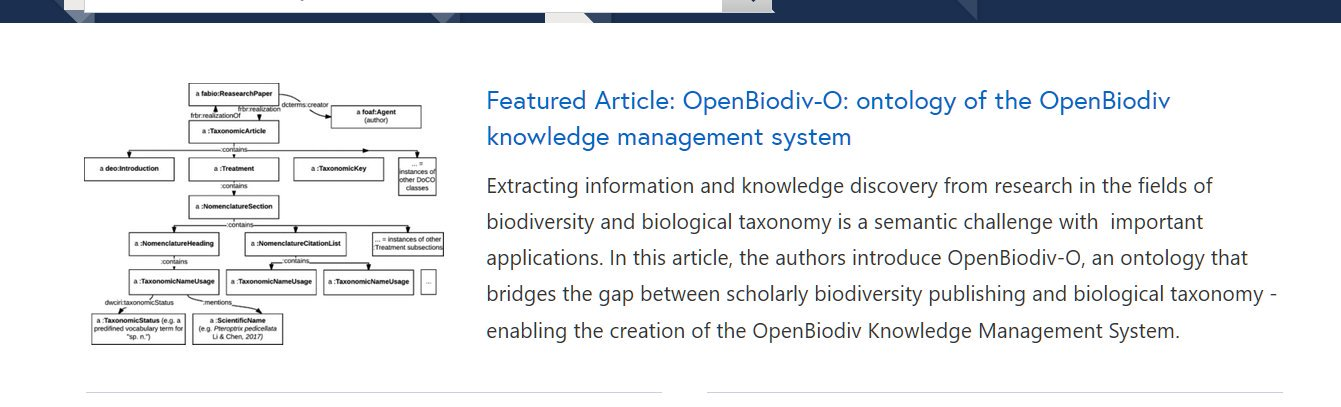
\includegraphics[width=\textwidth]{Figures/JBS-featured.jpg}
\decoRule
\caption{The OpenBiodiv-O article is featured on the main webpage of the Journal of Biomedical Semantics..}
\label{fig:jbs-featured}
\end{figure}

\section*{Апробация на резултатите}
\addcontentsline{toc}{section}{Апробация на резултатите}

\subsection*{Доклади пред научен семинар на ПНЗ}
\addcontentsline{toc}{subsection}{Доклади пред научен семинар на ПНЗ}

\begin{enumerate}
    \item Доклад пред научен семинар на ИБЕИ на БАН на 26.10.2015 г. (“Публикуване, визуализация и разпространение на първични и геномни данни за биологичното разнообразие на основата на открита система за управление на информацията”).
    \item Доклад пред научен семинар в ИИКТ на БАН на 31.03.2016 г. (Open Biodiversity Knowledge Management System)
    \item Dоклад пред научен семинар на ИИКТ на БАН за 23.03.2018 г. (OpenBiodiv: a knowledge-based system of biodiversity information)
\end{enumerate}

\subsection*{Доклади пред научно мероприятие в чужбина или пред международно научно мероприятие у нас}
\addcontentsline{toc}{subsection}{Доклади пред научно мероприятие в чужбина или пред международно научно мероприятие у нас}

\begin{enumerate}
    \item Доклад пред международния симпозиум EU BON в София на 23.03.2016 г. (The Data Publishing Toolkit at EU BON: Automated creation of data papers, data and text integrated publishing via the ARPHA Publishing Platform.)
    \item Доклад по време на работната среща на BIG4 в Хавраники, Чехия на 03.06.2016 г. (Project Progress Report (OBKMS))
    \item Доклад по време на работната среща на BIG4 в Хавраники, Чехия на 03.06.2016 г. (Modern Methods of Systematic Research and the BOLD Algorithm)
    \item Уеб-базиран доклад (уебинар) пред международна аудитория в рамките на семинар на iDigBio на 16.07.2016 г. (Online direct import of specimen records from iDigBio instrastructure into taxonomic manuscripts)
    \item Доклад по време на работната среща на BIG4 в Копенхаген на 14.10.2016 г. (Midterm Progress Report)
    \item Доклад на международия симпозиум TDWG 2016 в Санта Клара де Сан Карлос от 5. до 9.12.2016 г. (Streamlining the Flow of Taxon Occurrence Data Between a Manuscript and Biological Databases)
    \item Доклад на международия симпозиум TDWG 2016 в Санта Клара де Сан Карлос от 5. до 9.12.2016 г. (The Open Biodiversity Knowledge Management System: A Semantic Suite Running on top of the Biodiversity Knowledge Graph)
    \item Доклад на международия симпозиум TDWG 2016 в Санта Клара де Сан Карлос от 5. до 9.12.2016 г. (Demonstrating the Prototype of the Open Biodiversity Knowledge Management System)
    \item Доклад на международия симпозиум TDWG 2016 в Санта Клара де Сан Карлос от 5. до 9.12.2016 г. (Creation of Data Paper Manuscripts from Ecological Metadata Language (EML))
    \item Уеб-базиран доклад пред междуродния семинар на работната група по семантични технология към Университета Вандербилт (Тенеси, САЩ) на 20.02.2017 г. (Open Biodiversity Knowledge Management System)
    \item Доклад на европейската конференция на биосистематиците, BioSyst.eu 2016 на 15.08.2017 г. (The OpenBiodiv Knowledge System: The Future of Access to Biodiversity Knowledge)
    \item Доклад на международия симпозиум TDWG 2017 в Отава, Канада от 1. до 6.10.2017 г. (OpenBiodiv Computer Demo: an Implementation of a Semantic System Running on top of the Biodiversity Knowledge Graph)
    \item Доклад на международия симпозиум TDWG 2017 в Отава, Канада от 1. до 6.10.2017 г. (OpenBiodiv: an Implementaion of a Semantic System Running on top of the Biodiversity Knowledge Graph)
    \item Постер на международия симпозиум TDWG 2017 в Отава, Канада от 1. до 6.10.2017 г. (OpenBiodiv: an Implementaion of a Semantic System Running on top of the Biodiversity Knowledge Graph)
    \item Доклад по време на работната среща на BIG4 в Ла Палма, Испания от 30. окт. до 3 ноем. 2017 г. (Midterm Progress Report)
    \item Доклад пред научен семинар на групата по биоинформатика (група Ронкуист) в Кралския природо-научен музей в Стокхолм на 29.11.2017 г.
\end{enumerate}

\section*{Main scientific and applied contributions}
\addcontentsline{toc}{section}{Main scientific and applied contributions}

In the course of the investigative effort, all six objectives have been achieved and the results have been published in international journals and have been presented at major conferences in Bulgaria and abroad. The most important contributions of the thesis are summarized as follows:

\section*{Декларация за оригиналност}
\addcontentsline{toc}{section}{Декларация за оригиналност}

Декларирам, че настоящата дисертация съдържа оригинални резултати, получени 
при проведени от мен научни изследвания, с подкрепата и съдействието на научния ми ръководител проф. Любомир Пенев и Издаделство Пенсофт, както и научния ми консултант доц. Кирил Симов и ИИКТ.  Резултатите,  които  са  получени,  описани  и/или  публикувани  от  други учени, са надлежно и подробно цитирани в библиографията.

Настоящата дисертация не е прилагана за придобиване на научна степен в друго 
висше училище, университет или научен институт.

Виктор Сендеров

%----------------------------------------------------------------------------------------
%	ACKNOWLEDGEMENTS
%----------------------------------------------------------------------------------------

\begin{acknowledgements}
\addchaptertocentry{\acknowledgementname} % Add the acknowledgements to the table of contents

This research has been financed through the European Union’s Horizon 2020 research and innovation program under the Marie Sklodowska-Curie grant agreement No. 642241. My deep gratitude goes to the European Commission for enabling this wonderful opportunity!

\vspace{5mm}

I thank Prof. Lyubomir Penev and Prof. Kiril Simov for the valuable supervision. I also thank the staff and developers at Pensoft Publishers for the support in creating the platform and its popularization; in particular Prof. Pavel Stoev, Teodor Georgiev, Georgi Zhelezov, Iliyana Kuzmova, and Iva Kostadinova. Furthermore, I thank Pensoft's graphic designer, Slavena Peneva, for the help with creating the illustrations for this thesis and in presentations. Last but not least, Margarita Grudova and Elisaveta Taseva for providing valuable administrative support during the elaboration of the thesis.

\vspace{5mm}

I thank my colleagues from the Bulgarian Academy of Sciences (Institutes for Information and Communication Technologies and for Biodiviversity and Ecosystems Research) for their friendship and advice; in particular Prof. Galya Angelova, Prof. Boyko Georgiev, and Prof. Snejana Grozeva.

\vspace{5mm}

I thank my colleagues at the BIG4 training network for the feedback, friendship, and support. In particular Prof. Alexey Solovdnikov, but there are too many more names to mention.

\vspace{5mm}

I thank my international collaborators for their ideas, reviews, and collaboration on papers. In particular Prof. Nico Franz (Arizona State University), Dr. Daniel Mietchen (National Institutes of Health), Dr.  Éamonn Ó Tuama (formerly at GBIF), and Prof. Bob Morris (emeritus UMASS).

\vspace{5mm}

I also thank everyone at Plazi for the co-ownership of the vision of the project; in particular, Dr. Donat Agosti, Terry Catapano, and Dr. Guido Sautter.

\vspace{5mm}

Last but not least, I would like to acknowledge Ontotext for building the GraphDB database and providing excellent support.



\end{acknowledgements}
\chapter{Резюме на глава 1: Архитектура на OpenBiodiv}
\label{chapter-openbiodiv}

В тази глава предоставяме архитектурата, т.е. спецификацията и дизайна на OpenBiodiv. Въвеждаме компонентите на OpenBiodiv, които ще бъдат разгледани подробно в следващите глави. Описваме как взаимодействат тези компоненти, за да се формира базираната на знанието система OpenBiodiv.

\section{Какво е OpenBiodiv?}

Разбирането за OpenBiodiv като система базирана на знанието може да се обобщи по следния начин: OpenBiodiv е база данни от взаимосвързана информация за биологичното разнообразие, заедно с логика и приложения, позволяващи на потребителите не само да се допитват до данните, но и да откриват допълнителни факти, свързани с данните. Основните източници на информация в OpenBiodiv са списанията на академичния издател Пенсофт, таксономичната информация от Плаци и таксономичният гръбнак на Global Information Biodiversity Facility (GBIF).

Изследователският проблем на архитектурата на OpenBiodiv може да се формулира като проектиране на семантична графична база данни на основата на RDF. Тя да е с отворен достъп и да включва информация, предоставяна от Пенсофт, Плаци и GBIF, и да позволява на потребителите на системата да задават сложни заявки.

OpenBiodiv се състои от (1) семантична графична база данни, (2) програмен код, осигуряващ функционирането на базата и (3) динамична уеб страница (front-end), улесняваща достъпа до основната база от знания (Фиг.~\ref{fig:openbiodiv-components}). OpenBiodiv позволява динамичното вмъкване на данни от хранилища за данни за биологичното разнообразие в текста на статия в Biodiversity Data Journal или друго списание, използващи фреймуорка на Пенсофт за писане на статии, ARPHA-BioDiv (\cite{penev_arpha-biodiv:_2017}). Като втора стъпка, от тези списания се извлича знание, като се възползваме от XML-схемата на тези списания (TaxPub). Списания, които са извлечени, включват ZooKeys, Biodiversity Data Journal (BDJ), PhytoKeys, MycoKeys и т.н.\footnote{Списанията могат да бъдат достъпвани под \url{https://pensoft.net/browse_journals}}. В същото време знание под формата на факти (трипъли) се извлича от Plazi TreatmentBank, архив на литература за биологичното разнообразие, съдържащ над 200 хиляди таксономични дискусии\footnote{Таксономичната дискусия е специален раздел в биологична публикация, която описва и дискутира вид или по-висок таксон. TreatmentBank е достъпен под \url{https:// //plazi.org/resources/treatmentbank/}} и актуализиран всеки ден. Не на последно място, тези факти са взаимосвързани чрез таксономичния гръбнак на GBIF (\cite{gbif_secretariat_gbif_2017}). След това извлеченото знание се съхранява в нашата семантична база данни  (Фиг.~\ref{fig:openbiodiv-sources}).

\begin{figure}
\centering
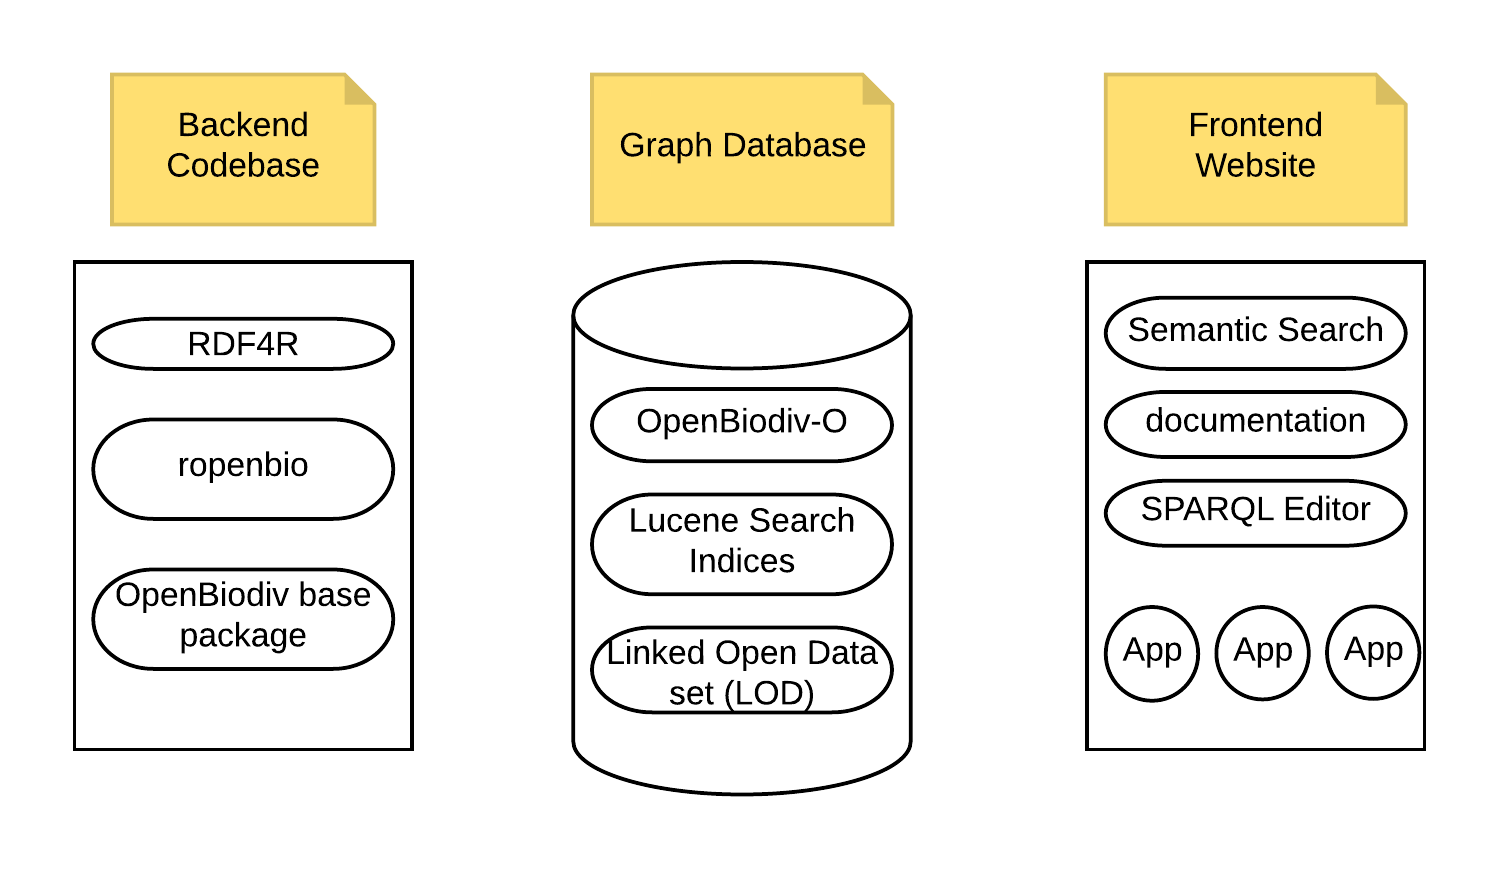
\includegraphics[width=\textwidth]{Figures/components-openbiodiv}
\decoRule
\caption[OpenBiodiv Components]{Компоненти на OpenBiodiv.}
\label{fig:openbiodiv-components}
\end{figure}

\begin{figure}
\centering
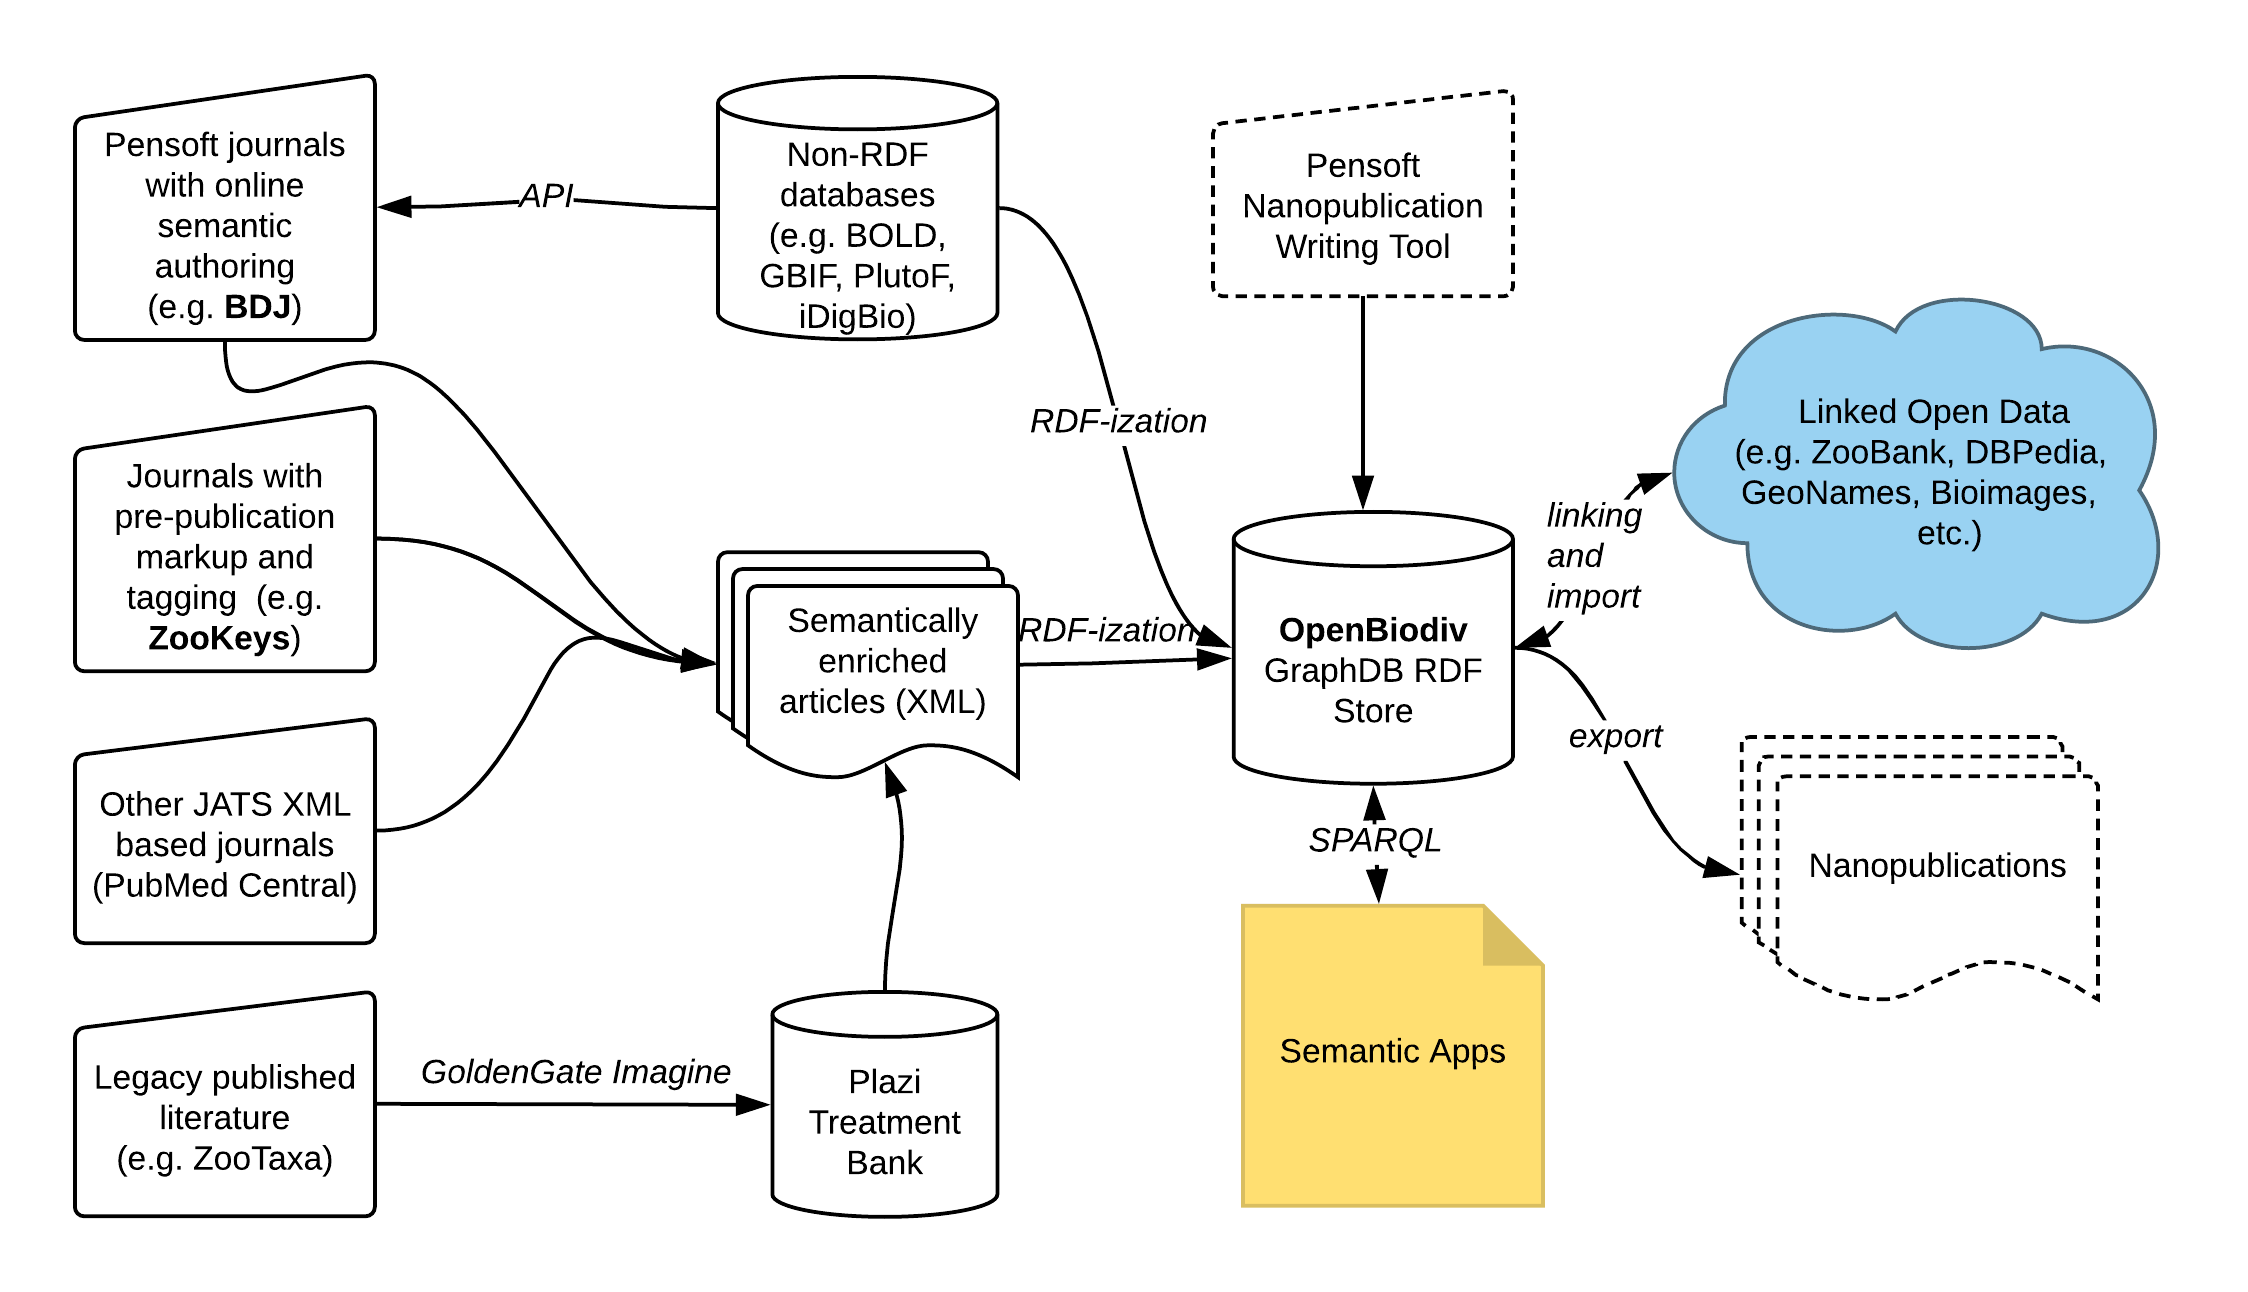
\includegraphics[width=\textwidth]{Figures/openbiodiv-sources}
\decoRule
\caption[OpenBiodiv Components]{Поток на информация в пространството за данни за биологичното разнообразие. Пунктираните линии са компоненти, които все още не са създадени.}
\label{fig:openbiodiv-sources}
\end{figure}

\section{Семантична база данни}

Основен резултат от усилията на OpenBiodiv е създаването на семантична база данни, базирана на знания, извлечени от архивите на Пенсофт и Плаци и таксономичния гръбнак на GBIF и достъпни под \url{http://graph.openbiodiv.net/}. Следва обсъждане на компонентите на базата данни.

\subsection{Онтология OpenBiodiv-O}

Централният резултат от усилията по OpenBiodiv е създаването на формален модел на областта за публикуването на знание за биоразнообразието. Този формален модел е онтологията OpenBiodiv-O (\cite{senderov_openbiodiv_2017}). Изходният код на онтологията и придружаващата документация могат да бъдат достъпвани под \url{https://github.com/pensoft/openbiodiv-o}. Детайлна дискусия е представена в глава~\ref{chapter-ontology}.

\subsection{Свързани отворени данни OpenBiodiv-LOD }

Използвайки OpenBiodiv-O и инфраструктурата, описана по-нататък в тази глава, са създадени свързани отворени данни, включващи приблизително 200 хиляди записа от Плаци, пет хиляди статии от Пенсофт, както и таксономичия гръбнак на GBIF (над милион биологични имена). Данните са достъпни онлайн чрез работния инструмент на семантичната база данни \url{http://graph.openbiodiv.net}. Разясняват се подробно в глава~\ref {chapter-lod}.

\section{Backend}

За да се попълва семантичната база данни, е необходимо да се създаде инфраструктура, която преобразува необработени данни (текст, изображения, таблици с данни и т.н.) в структуриран семантичен формат. OpenBiodiv предоставя инфраструктура за трансформиране на научни публикации за биоразнообразието в твърдения под формата на RDF с помощта на инструментите, описани в този раздел.

\subsection{RDF4R: R пакет за работа с RDF}

Едно от по-големите технически предизвикателства за OpenBiodiv е трансформирането на информация за биологичното разнообразие (напр. таксономични имена, метаданни, фигури и т.н.), съхранявани като полу-структуриран XML в напълно структурирани семантични знания под формата на RDF. За да се реши това предизвикателство, е разработен R пакет, който позволява създаването, манипулирането и записа в семантична база данни на създадения RDF. Този пакет е достъпен под лиценз с отворен код на GitHub под \url{https://github.com/vsenderov/rdf4r}. Описваме пакета в глава~\ref{chapter-rdf4r}.

\subsection{Базисен програмен код и ROpenBio}

В комбинация с пакета RDF4R, програмният код съдържа още един R пакет, \cl{ropenbio} и базисен програмен код от скриптове и документация, необходими за стартиране на базата данни. \cl{ropenbio} използва пакета RDF4R за преобразуване на полу-структуриран XML в RDF. Той съдържа преобразуванията, необходими за тази реализация. Той е достъпен под \url{https://github.com/pensoft/ropenbio}. Базисният софтуерен код координира извикването на \cl{ropenbio}, съдържа скриптове за автоматично импортиране на нови ресурси и други подробности. Той е достъпен под \url{https://github.com/pensoft/openbiodiv}. Генерирането на OpenBiodiv-LOD с помощта на тези пакети е обсъдено в глава~\ref{chapter-lod}.

\subsection{Работен процес за преобразуване на екологични метаданни в ръкопис}

Език за екологични метаданни (EML) е популярен формат за описване на екологични данни (\cite{michener_nongeospatial_1997}). Хранилища на данни за биоразнообразието, като GBIF и DataOne, използват този формат за метаданните, които съхраняват. Автоматичното преобразуване на EML файл в data paper ръкопис от Biodiversity Data Journal\footnote {Data paper (\cite{chavan_data_2011}) е научна статия, обсъждаща научни данни.} е възможно с помощта на системата OpenBiodiv (\cite{senderov_online_2016}). Този работен процес е описан подробно в глава~\ref{chapter-case-study}\footnote{За работа в интерактивен режим, отидете на \url{https://arpha.pensoft.net}, влезте в системата (регистрацията е безплатна), изберете ``Start a new manuscript'', превъртете до ``Import manuscript'' и следвайте необходимите стъпки, за да качите EML файл и да го използвате като шаблон за вашия нов ръкопис.}.

\subsection{Работен процес за импортиране на данни за наблюдения на видове в ръкопис}

Един от важните видове данни за биологичното разнообразие са данни за наблюдения на организми, occurrence data. Това са данни, които документират наличието на правилно таксономично идентифициран организъм на дадено място и време. Такива данни се съхраняват в международни хранилища като BOLD, GBIF, PlutoF и iDigBio. За да се улесни публикуването на такъв тип данни е разработен работен процес за импортиране на такива записи от тези бази данни в таксономична статия (taxonomic paper) в списанието Biodiversity Data Journal (\cite{senderov_online_2016}). Този работен процес е описан подробно в глава~\ref{chapter-case-study}\footnote{За да отворите интерактивно работния процес, отидете на \url{https://arpha.pensoft.net}, влезте в системата (регистрацията е безплатна), изберете ``Start a new manuscript'', изберете ``Biodiveristy Data Journal'', ``Taxonomic paper''  и ``Create a new manuscript''. След това в новия ръкопис щракнете с мишката върху раздела ``Taxon treatments'', като кликнете върху знака $+$ до него, и укажете биологичната класификация на новия запис (напр. Animalia), и най-накрая щракнете върху ``Save'' и ще ви бъде представен избор на подраздели. Кликнете върху секцията ``Materials'' от-вляво, за да видите инструмента на работния процес за вмъкване на материли. Погледнете в долната част на диалоговия прозорец, където можете да поставите множество идентификационни номера. Това е частта, в която избирате външни идентификатори на ресурси, които да бъдат импортирани във вашата статия.}.

\section{Интерфейс}

В допълнение към предоставения endpoint за база данни с възможност за търсене, се разработва уебсайт, позволяващ семантично търсене и капсулиращ специфични задачи, пакетирани като приложения (\url{http://openbiodiv.net}). Бета версията вече е в действие. Фиг.~\ref{fig:website}. Ограничена дискусия е представена в глава~\ref{chapter-webportal}.

\section{Системна администрация}

Системата е разположена на виртуална машина на Debian GNU+Linux. GraphDB работи с heap файл от 20 GB и с набор от правила RDFS-Plus Optimized. Това се налага поради факта, че достигнахме препятствия, когато използвахме OWL извод. Обсъдени в глава~\ref {chapter-lod}. Непрекъснатата работа се осигурява от автоматичното изпълнение на скриптове от директорията \cl{run} на базисния код на OpenBiodiv.

\begin{figure}
\centering
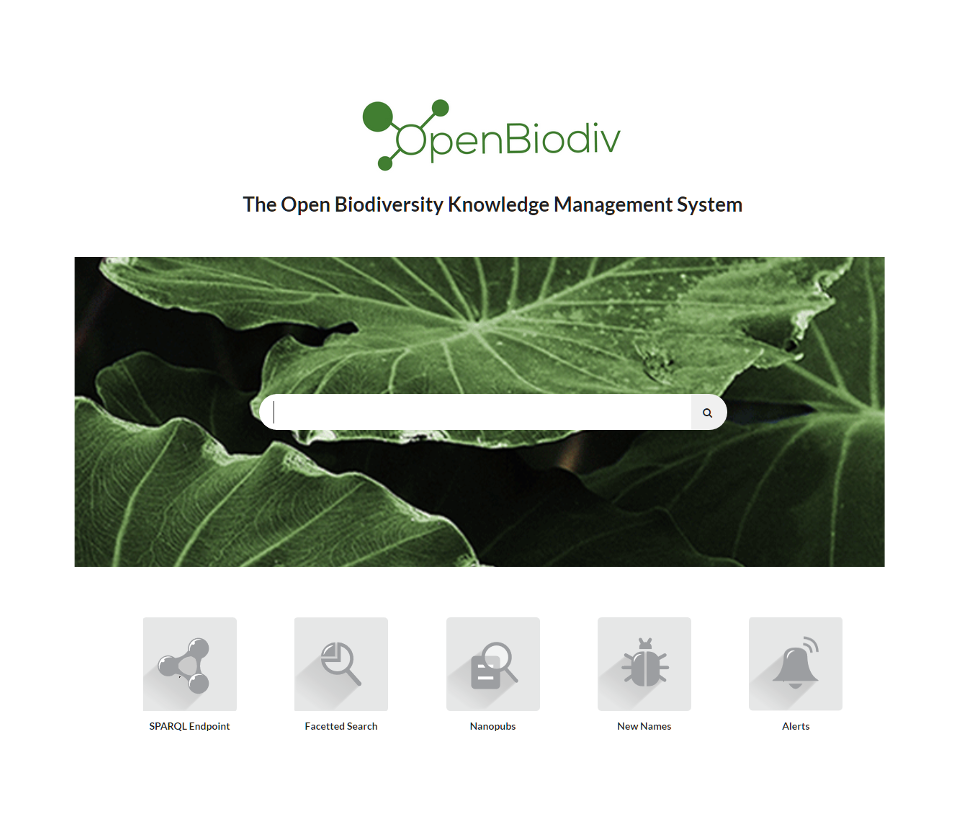
\includegraphics[width=\textwidth]{Figures/openbiodiv-webpage}
\decoRule
\caption[OpenBiodiv Website]{Бета версия на потребителския интерфейс.}
\label{fig:website}
\end{figure}

\section{Дискусия}

Проектирането на системата започна във втората половина на 2015 г., когато бяха разгледани различни алтернативи за база данни (Neo4J, GraphDB, WikiBase) и различни технологии за RDF-изация на знание. Освен това беше направен избор на източници за информация и типове данни, които са интересни. Бяха разгледани основните модели данни и онтологии. След този анализ, публикувахме спецификацията на системата в \cite{senderov_open_2016} като отворен проект за дисертация (PhD project plan). По време на имплементацията обаче се оказа, че първоначалният план не отговаря на изменящите се изисквания на системата и на новите предизвикателства, които възникваха по време на имплементацията. По тази причина през втората и третата година на усилията за създаване на OpenBiodiv преминахме от модела на разработка waterfall, където след първоначален етап на изготвяне на софтуерната архитектура се преминава към продължителен етап на имплементация и тестване към модела agile, където спецификацията е разбита на по-малки user-stories, които биват реализирани ad-hoc в рамките на едно- или двумесечни спринтове. Например, за разработването на софтуерната библиотека за RDF-изация RDF4R, user-stories са ``възможност за работа с литерали'', ``възможност за импортиране през API endpoint'' и т.н. Първоначалният страх, че това ще доведе до ``хакерски код'' и недобре организирана софтуерна архитектура се оказа неоправдан, защото при изолирането на проблемите един от друг, успявахме да се концентираме върху проблемите последователно и да ги решаваме по елегантен начин. Аспекти на методологията agile, от които не успяхме да се възползваме напълно бяха колаборативните аспекти, може би поради факта, че системата беше разработена основно от кандидата със съдействието на един от програмистите на Пенсофт; в класическия смисъл на понятието agile team не съществуваше. По тази причина не практикувахме повечето ритуали като stand-ups и retrospection, а основно се концентирахме върху интеративния характер на разработката на софтуер.

Нашата визия за бъдещето на системата е работата по нея да се поеме от agile team, който да се възползва от пълния арсенал на методологията.
\chapter{Резюме на глава 2: Онтологията на OpenBiodiv}
\label{chapter-ontology}

OpenBiodiv трансформира информация за биоразнообразието от научни публикации и академични бази данни в семантичен вид. В тази глава представям OpenBiodiv-O (\cite{senderov_openbiodiv-o:_2018}) - онтологията, формираща модела на OpenBiodiv за знания и извод. OpenBiodiv-O предоставя концептуален модел на структурата на академична публикация в сферата на биоразнообразието и на съдържаните в нея таксономични концепции. За първи път формално е концептуализирана областта на публикуването на данни за биоразнообразието.

Чрез разработването на онтология, насочена към биологичната таксономия са запълнени празнините между онтологии като Darwin-SW и онтологиите за семантично публикуване като онтологиите SPAR. Считам, че е предимство да се моделира самият таксономичен процес, а не някакво конкретно състояние на знанието.

Изходният код и документацията са достъпни под лиценза CC BY \footnote {Creative Commons Attribution 4.0 International Public License} от GitHub \footnote {\url{https://github.com/vsenderov/openbiodiv-o/blob/master/LICENSE.md}}. Започваме с увод в областта на биологичната таксономия и свързаните с нея биоразнообразие.

\section{Концептуализация на областта}

Представям историята на модерната биологична таксономия, като се започне с Карл Линней (1707-1778), който предложи модерното групиране на организма на \emph{царства, класове, разреди, родове} и използването на латинските биномични имена в \emph{Systema Naturae} (\cite {linnaeus_systema_1758}). Подчертавам, че работата на таксономите за описване и организиране на биоразнообразието далеч не е пълна. Това информира създаването на новата онтология не като статично формализиране на съществуващата биологична таксономия в компютърно четима форма, а като формализиране на \emph{научния процес на биологичната таксономия}.

След това описвам подробно, как протича научният процес в биологичната таксономия. Започвам с въвеждането на таксономични концепции и начина, по който се формират. Таксономичната концепция е научна хипотеза (\cite{deans_time_2012}), че определена група от организми съществува в природата. Тя се формира чрез изследване на екземпляри и задължително включва научен критерий по който те да се групират, често наричан видова концепция (\cite {mallet_species_2001}) Исторически погледнато, организмите могат да бъдат групирани по външен вид и вътрешно устройство (концепция за морфологични видове) или репродуктивно поведение (биологична видова концепция), но напоследък фокусът се е насочил към групиране въз основа на генетична свързаност (филогенетични и геномни видови концепции).

След това описвам единците на биологичната таксономия и начина, по който те са регламентирани от международните кодекси \cite{international_commission_on_zoological_nomenclature_international_1999, noauthor_international_2012}). Кодексите уреждат по-ниските рангове: видове, род, семейство, разред; по-високите рангове (напр. отдел, царство, домейн и т.н.) могат да бъдат използвани от изследователите, както сметнат за подходящо. Това води до множество конкуриращи се гледни точки.

Публикуването таксономични концепции е неразделна стъпка в научния работен поток на всеки таксоном. Описваме структурата и типовете таксономични публикации, като се акцентираме специално върху секцията ``Таксономична дискусия'', раздела в таксономичната публикация, където таксономичната концепция е дефинирана.

\subsection*{Преглед на литературата}

В тази секция се разглеждат опитите областта на биологичната таксономия да бъде формално концептуализрана.  Интересни са SPAR Ontologies, \cite{peroni_semantic_2014}) и TaxPub XML Document Type Definition (\cite{catapano_taxpub:_2010}).

Концептуализацията основно е повлияна освен от практиката и от кодексите (\cite{international_commission_on_zoological_nomenclature_international_1999,noauthor_international_2012}), а така и от стандартите, създадени от TDWG (напр. Darwin Core, DwC, \cite{wieczorek_darwin_2012}).

Накрая правим обзор на областта на концептуалната таксономия (\cite{berendsohn_concept_1995, franz_perspectives:_2009,sterner_taxonomy_2017}), която представлява нова гледна точка за това, как трябва да протича процесът на опсване на видове в биологичната таксономия, с оглед на напредъка на информационните технологии.

\section{Методи}

OpenBiodiv-O се изразена посредством RDF чрез използване на RDF Schema (RDFS) и Web Ontology Language (OWL).

За да разработим онтологията ние използвахме следния процес: (1) анализ на областта и идентифициране на важните класове обекти и техните взаимоотношения (наричани свойства); (2) анализ на съществуващите информационни модели и онтологии и идентифициране на липсващите класове и свойства за успешно формализиране на областта.

\section{Резултати}

OpenBiodiv-O е \emph{споделена формална спецификация на концептуализация} на областта на биоразнообразието по смисъла на \cite{gruber_translation_1993, obitko_translations_2007, staab_handbook_2009}. Тяхното разбиране за онтология сме въвели в Background. 

Има няколко домейна, в които моделираните ресурси падат. Първият е научната област за публикуване на данни за биоразнообразието. Втората област е тази на таксономичната номенклатура. Третата област е на по-широката таксономия (например таксономични понятия и техните взаимоотношения, видови събития, черти).

\subsection{Семантично моделиране на домейна за публикуване на данни биоразнообразието}

Разширяваме рамката на онтологиите на SPAR, като въвеждаме нова категория за таксономичните статии, нейните подраздели, както и нов клас за споменаване на таксономично име (вж. следващ подраздел). Тези нови класове са обобщени в Таблица~\ref{bibliographic_classes}.

\begin{table}[h!]
\caption{Нови класове в областта на публикуването на данни за биоразнообразието.}
      \begin{tabular}{cc}
        \hline
          Class QName             & Comment\\  \hline
  {\tt :Treatment}                & section of a taxonomic article\\
  {\tt :NomenclatureSection}      & subsection of Treatment\\
  {\tt :NomenclatureHeading}      & contains a nomenclatural act \\
  {\tt :NomenclatureCitationList} & list of citations of related concepts\\
  {\tt :MaterialsExamined}        & list of examined specimens\\
  {\tt :BiologySection}           & subsection of Treatment\\
  {\tt :DescriptionSection}       & subsection of Treatment\\
  {\tt :TaxonomicKey}             & section with an identification key\\
  {\tt :TaxonomicChecklist}       & section with a list of taxa for a region\\ 
  {\tt :TaxonomicNameUsage}       & mention of a taxonomic name\\ \hline

      \end{tabular}
      \label{bibliographic_classes}
\end{table}

Графичното представяне на взаимоотношенията между ресурси на класовете, свързани с публикуването, които OpenBiodiv въвежда, може да се намери в диаграмата на фиг.~\ref{taxonomic-article-diagram}.

\begin{figure}[h!]
	\centering
	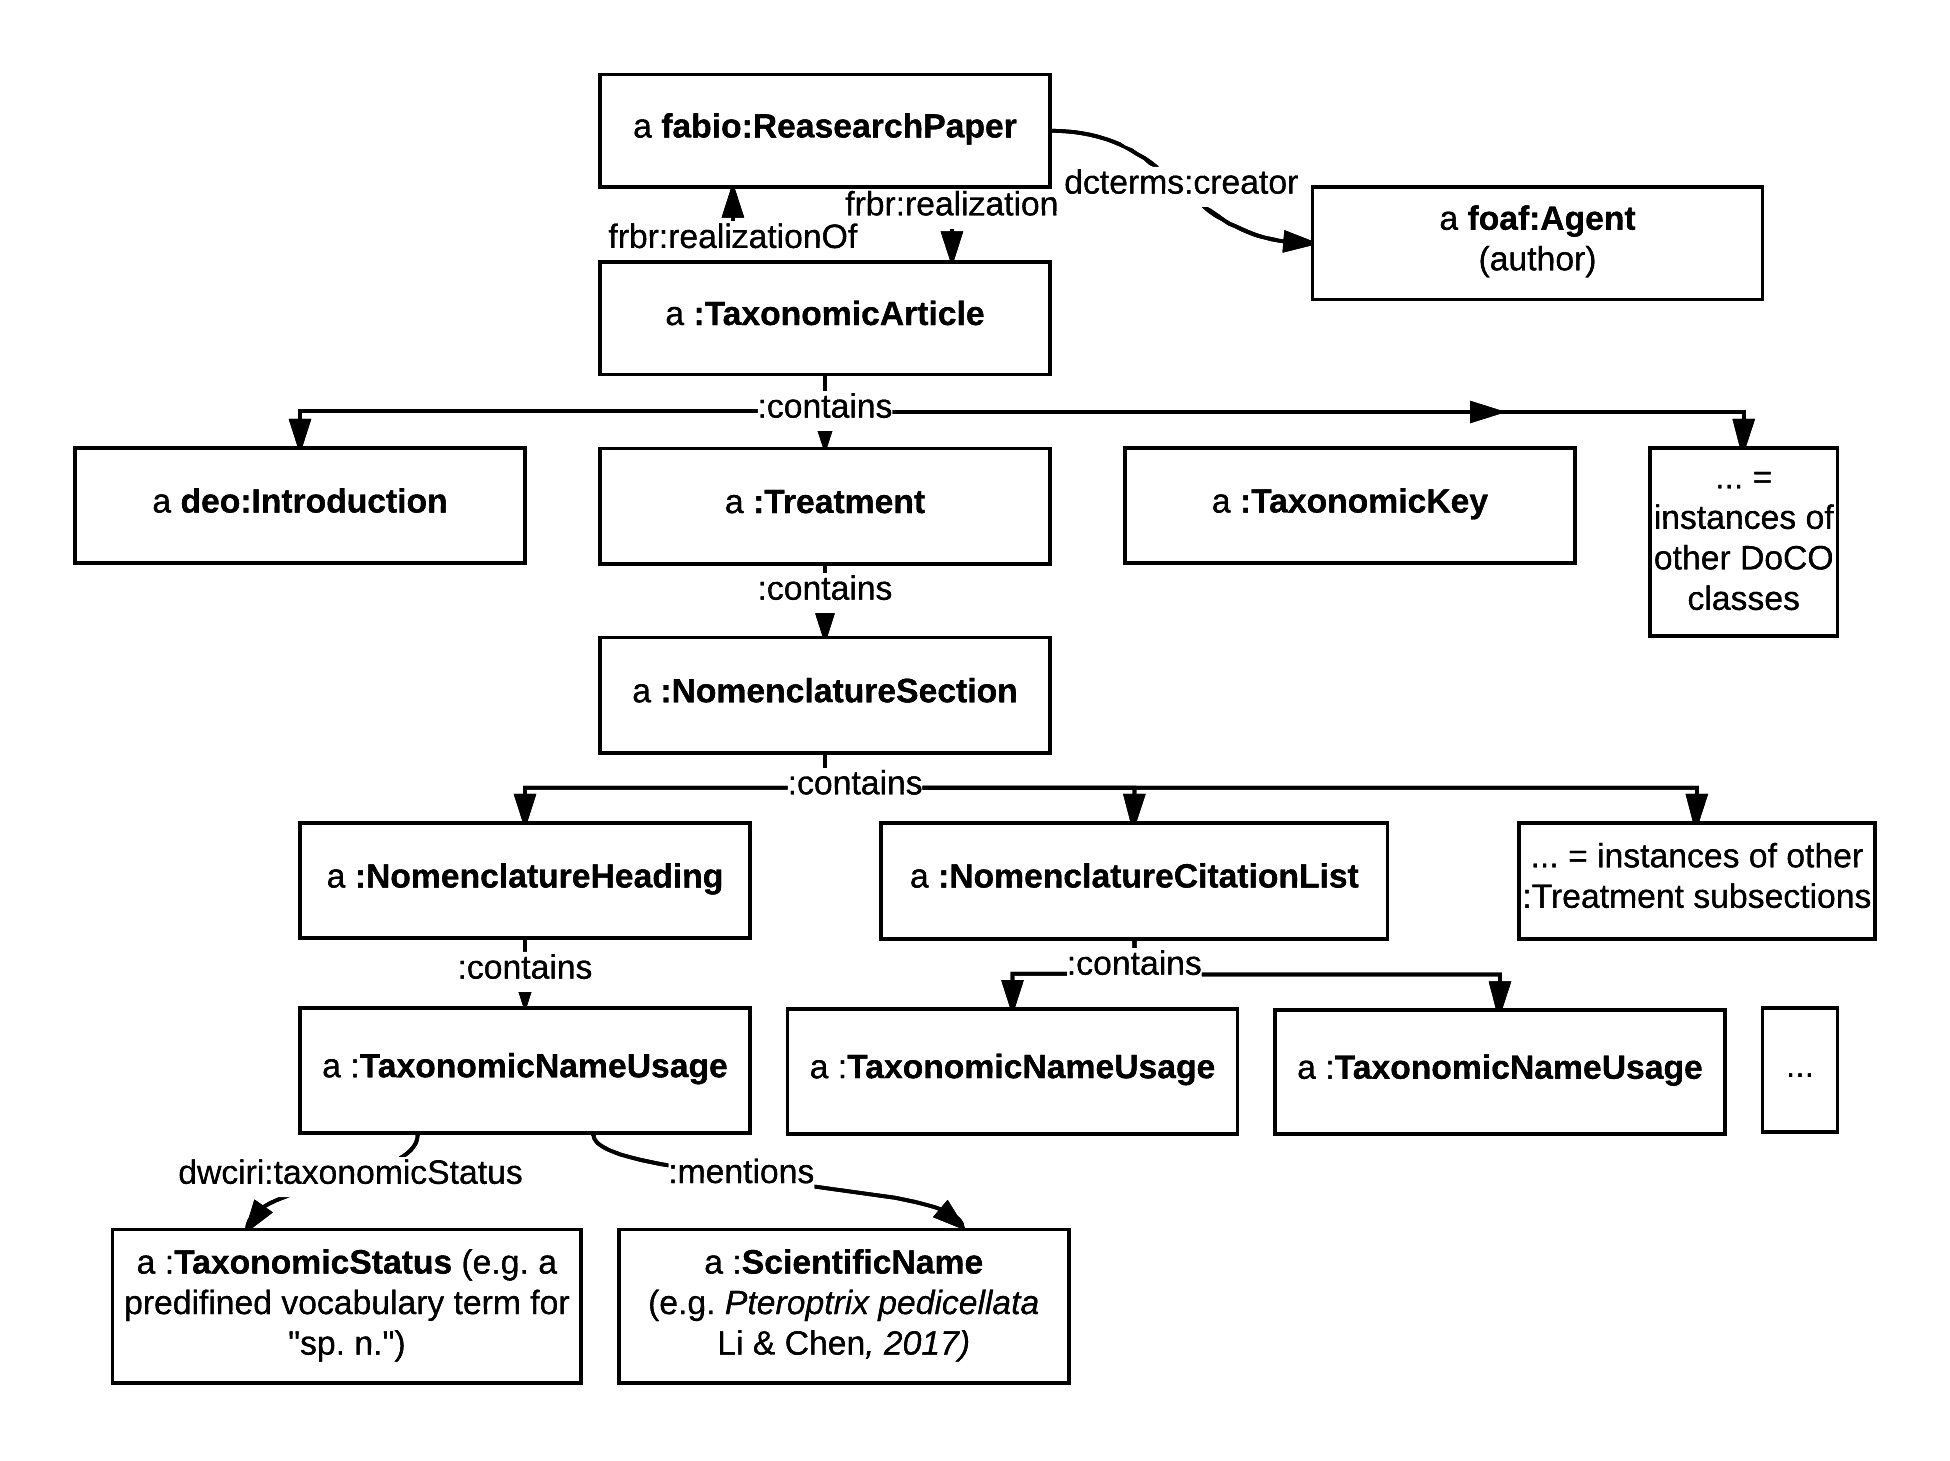
\includegraphics[width=\textwidth]{Figures/taxonomic-article-diagram}
	\decoRule
  \caption[Taxonomic article diagram.]{Графична репрезентация на взаимоотношенията между ресурсите, които OpenBiodiv въвежда за публикуване на данни за биоразнообразието.}
  \label{taxonomic-article-diagram}
\end{figure}

\subsubsection{Семантика и употреба}

В тази секция ние обсъждаме как класовете и свойствата, които въведохме, са в съответствие с модела на функционалните изисквания за библиографски записи (FRBR), използван от SPAR. Считаме дадена таксономична статия за конкретен израз/запис, FRBR Expression, на абстрактното понятие работа, FRBR Work, представляващо интелектуалното съдържание на статията. Таксономичната дискусия се третира подобно на Въведение, Методи, Резултати и т.н., т.е. също e FRBR Expression и DEO discourse element. Таксономична концепция е съответният абстрактен ресурс от клас FRBR Work на дадена таксономична дискусия. Фигурите~\ref{example-article-metadata} и \ref{example-article-structure} дават примерен сорс-код, илюстриращ тези идеи.

\begin{figure}[h!]
	\centering
	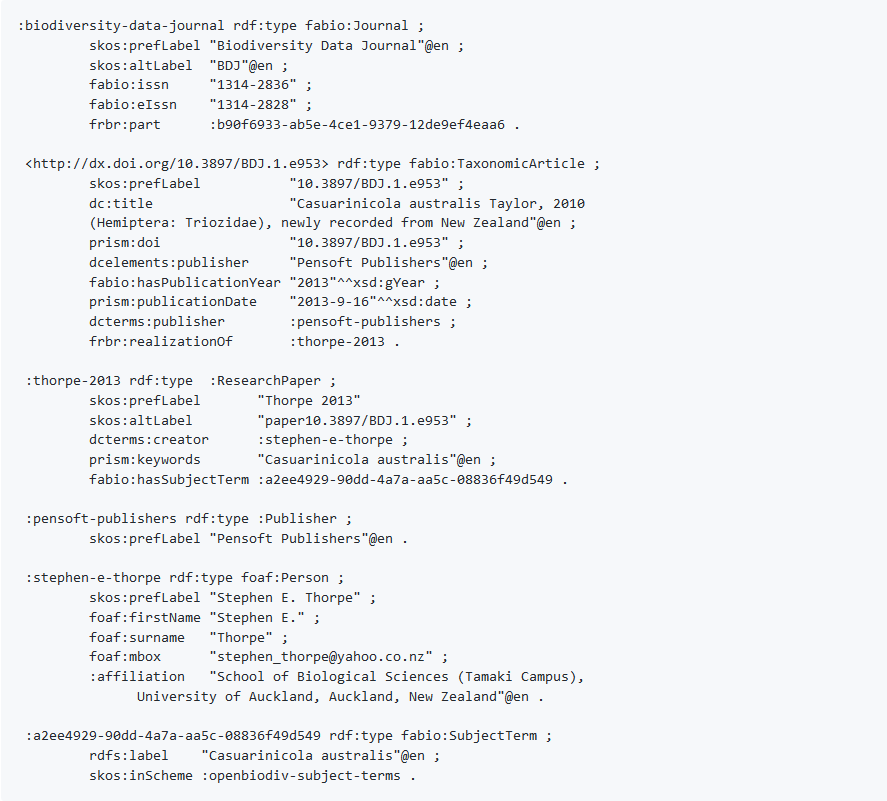
\includegraphics[width=\textwidth]{Figures/example-article-metadata}
	\decoRule
  \caption[Example article metadata.]{Този пример показва как да се изразят метаданните на таксономичната статия с модела на SPAR Ontologies и класовете, които OpenBiodiv определя. Кодът е на Turtle.}
  \label{example-article-metadata}
\end{figure}

\begin{figure}[h!]
  \centering
  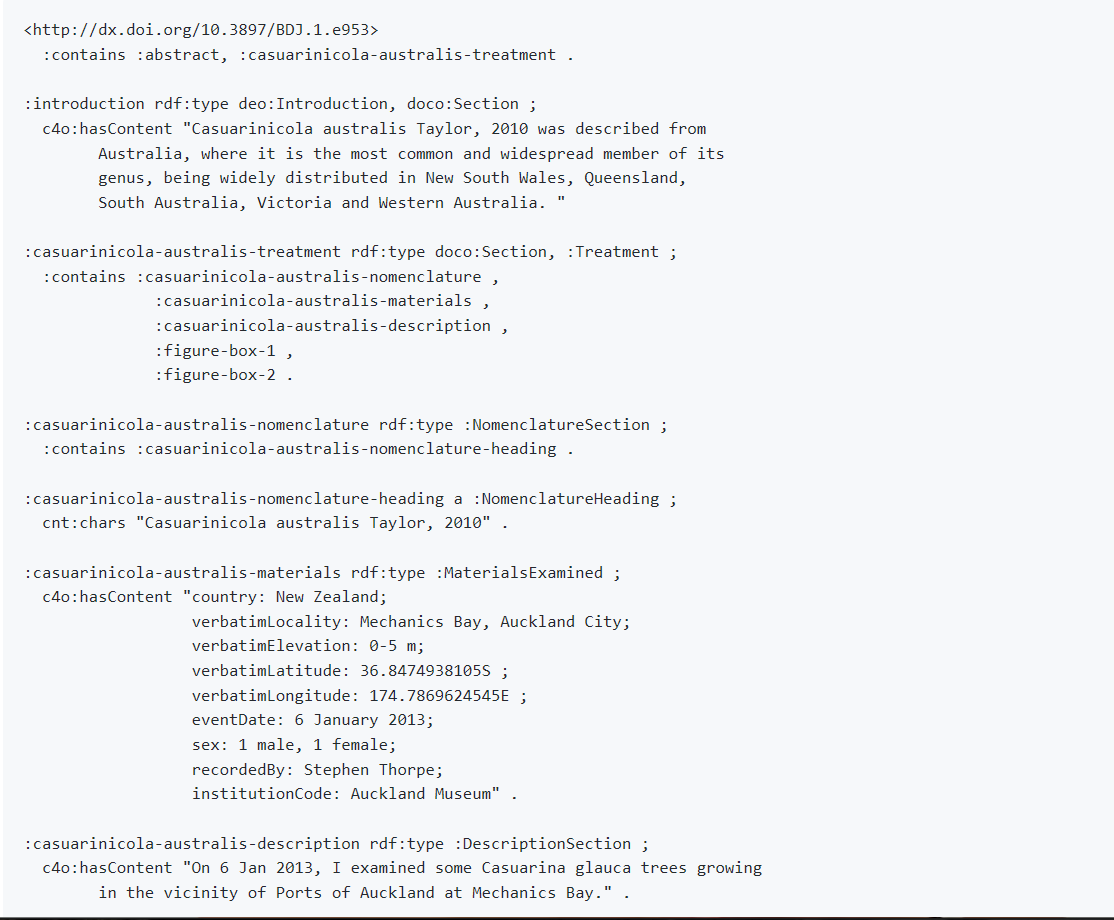
\includegraphics[width=\textwidth]{Figures/example-article-structure}
  \decoRule
  \caption[Example article structure.]{Този пример показва как да изразява структурата на статията с помощта на \cl{contains}. Кодът е на Turtle.}
  \label{example-article-structure}
\end{figure}


\subsection{Семантично моделиране на биологичната номенклатура}

Биологичната номенклатура е система с над 200 годишна традиция датираща до преди времето на информатиката и дори до преди времето на Теорията за еволюцията на Дарвин. Много е трудно да се моделира поради сложността си и само частично е обхваната от онтологиите NOMEN и TNSS (въведени в подраздел ``Previous Work''). С OpenBiodiv-O използвам подход "отдолу-нагоре" за моделиране на използването на таксономични имена в статиите. Където е възможно, ние подравняваме класовете OpenBiodiv-O на NOMEN.

Дефинирахме йерархията на класовете на таксономичните имена, намиращи се на фиг.~\ref{taxonomic-name-class-hierarchy-diagram}. Освен това въведехме taxonomic name usage (\cl{TaxonomicNameUsage}).

\begin{figure}[h!]
  \centering
  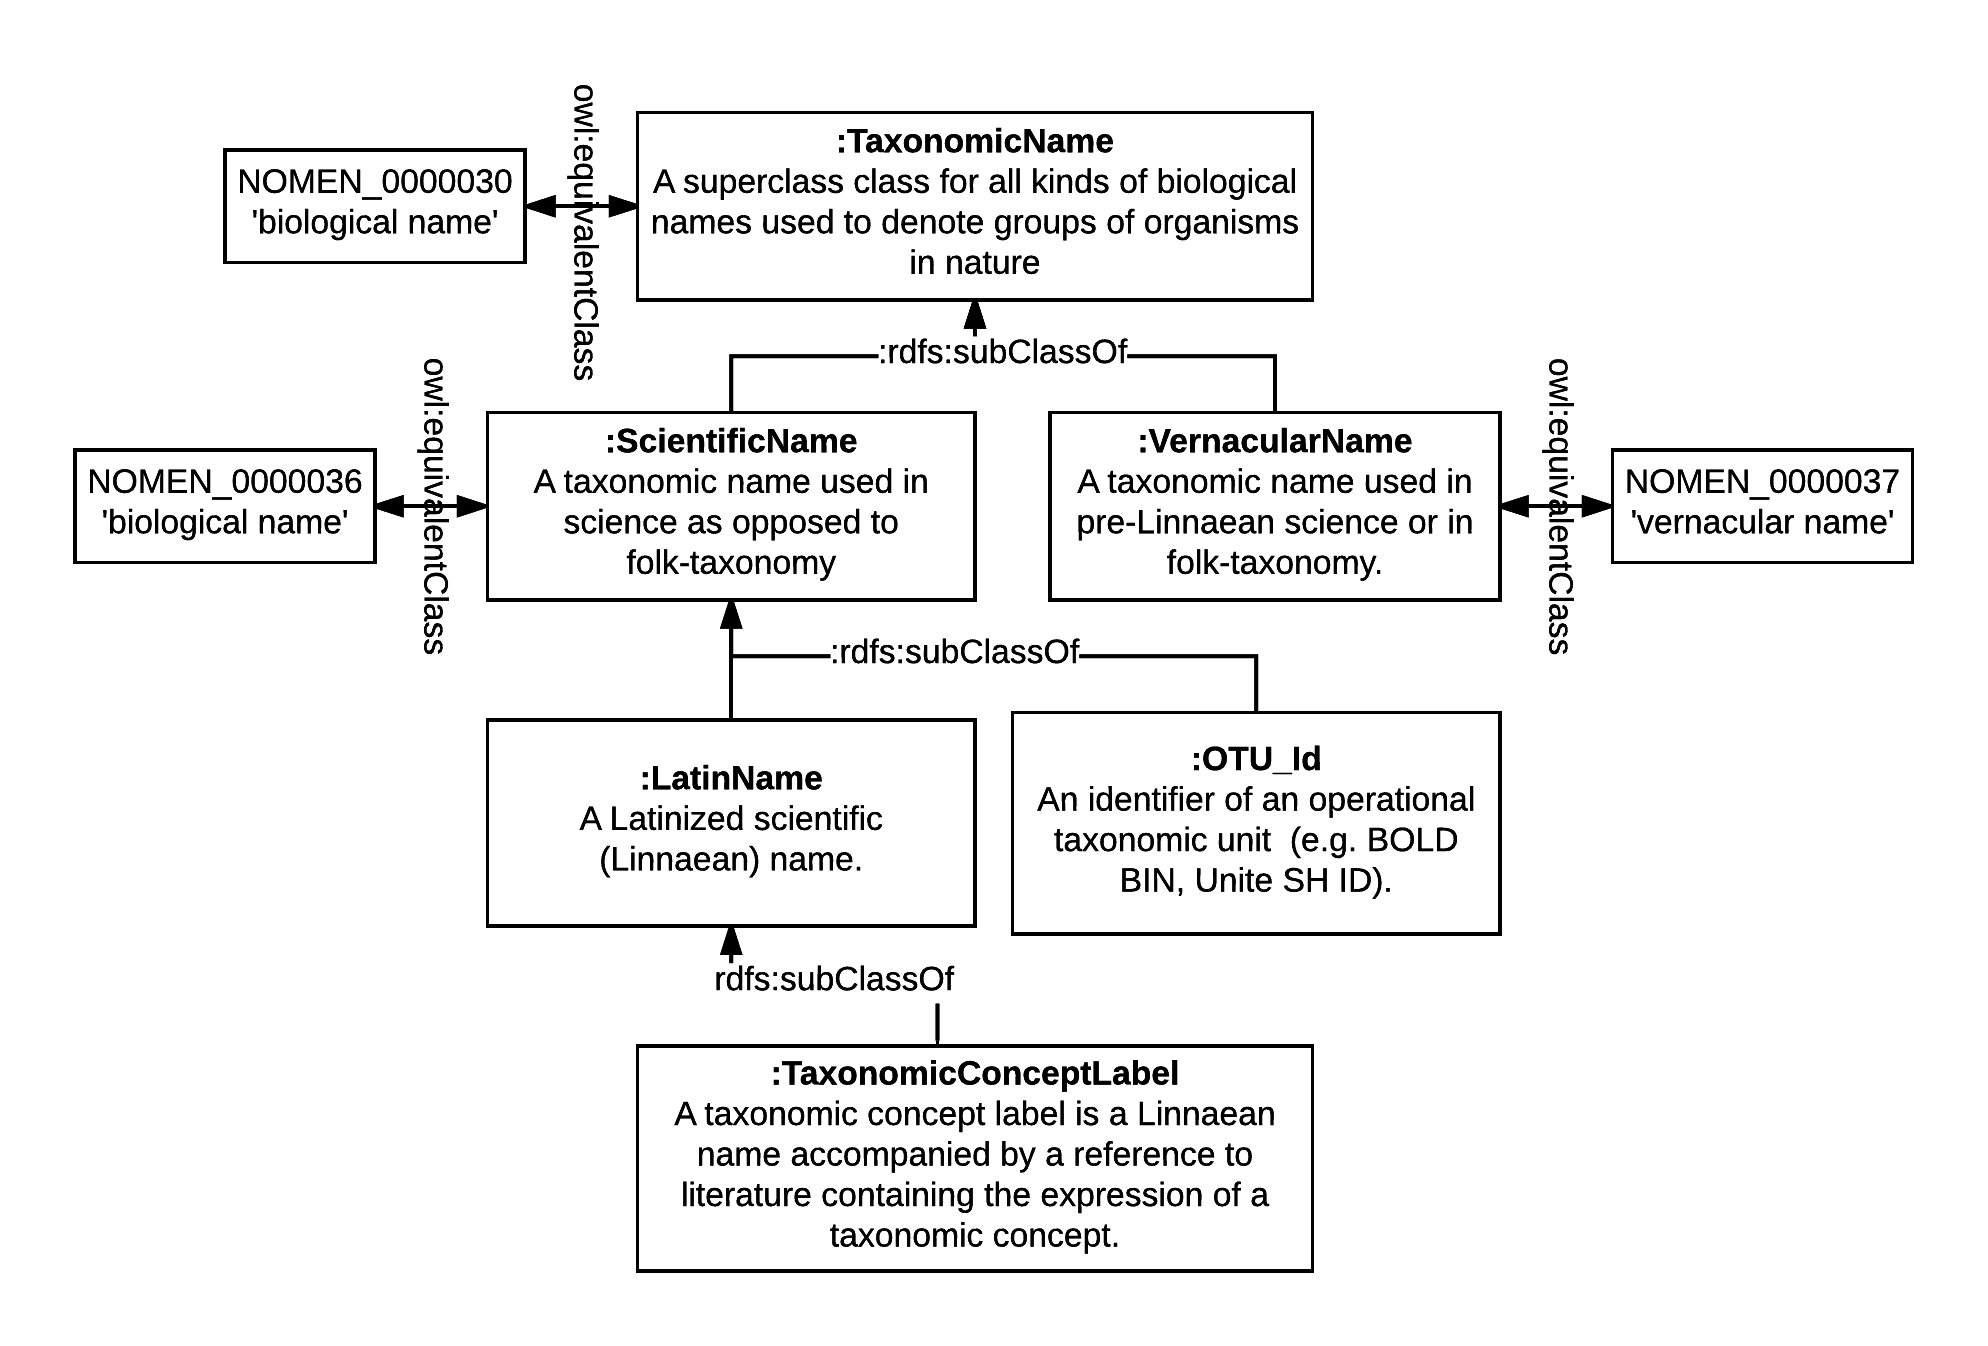
\includegraphics[width=\textwidth]{Figures/taxonomic-name-class-hierarchy-diagram}
  \decoRule
  \caption[Taxonomic name class hierarchy diagram.]{Създадохме тази йерархия, за да приспособим както традиционните таксономични наименования, така и използването на таксономични концептуални етикети и оперативни таксономични единици.}
  \label{taxonomic-name-class-hierarchy-diagram}
\end{figure}

Въвеждаме Taxonomic Concept Label (\cl{TaxonomicConceptLabel}). Етикетът на таксономична концепция (TCL) е линеево име плюс позоваване на публикация, където дискутираният таксон е дефиниран. Връзката се осъществява чрез ключовата дума ``sec.'' (Латинки за (\emph{secundum} \cite{berendsohn_concept_1995}). Напр. \emph{Andropogon virginicus} var. \emph{tenuispatheus} \cite{blomquist_grasses_1948}. Тук \cite{blomquist_grasses_1948} е валидна библиографска справка за публикацията, в която концепцията е дефинирана.

Извадихме съкращения от таксономични термини от около 4000 статии в четири таксономични списания (ZooKeys, Biodiversity Data Journal, PhytoKeys и MycoKeys), за да създадем таксономичен речник на термините, който обхваща осемте най-често срещани случая Таблица~\ref{taxonomic-status-vocabulary}). Латинските съкращения, които са класифицирани в тези класове, могат да бъдат намерени на страницата на OpenBiodiv-O GitHub. (Вижте Методи за повече подробности).

\begin{table}[h!]
\caption{Речник с таксономични термини.}
\begin{tabular}{ccc}
\hline
Vocabulary Instance QName & Example Abbrev & Comment\\ \hline
{\tt :TaxonomicUncertainty} & \emph{incertae sedis} & Taxonomic Uncertainty\\
{\tt :TaxonDiscovery} & \emph{sp. n.} & Taxonomic Discovery \\
{\tt :ReplacementName} & \emph{comb. n.} & Replacement Name \\
{\tt :UnavailableName} & \emph{nomen dubium} &  Unavailable Name \\
{\tt :AvailableName} & \emph{stat. rev.} & Available Name \\
{\tt :TypeSpecimenDesignation} & \emph{lectotype designation} & Type Specimen Designation \\
{\tt :TypeSpeciesDesignation} & \emph{type species} & Type Species Designation\\
{\tt :NewOccurrenceRecord} & \emph{new country record} & New Occurrence Record (for region)\\
\hline
\end{tabular}
\label{taxonomic-status-vocabulary}
\end{table}

Въз основа на нашия анализ на термините за таксономични статуси, идентифицирахме два модела за съответствие между кодирането на латинизираните научни имена (Фиг.~\ref{scientific-name-patterns}). Моделът \emph{заместващо име}, изпълняван чрез свойството \cl{replacementName}, показва, че вместо едно латинизирано име,  трябва да се използва друго. Тя обхваща голямо разнообразие от случаи в кодексите, като например поставянето на един вид таксон в нов род (нова комбинация), поправката на наименование поради номенклатурни причини (ново име), или прилагането на Принципа на приоритет за откриването на синоними ("syn nov.", \cite{international_commission_on_zoological_nomenclature_official_2017}).

\begin{figure}[h!]
 \centering
  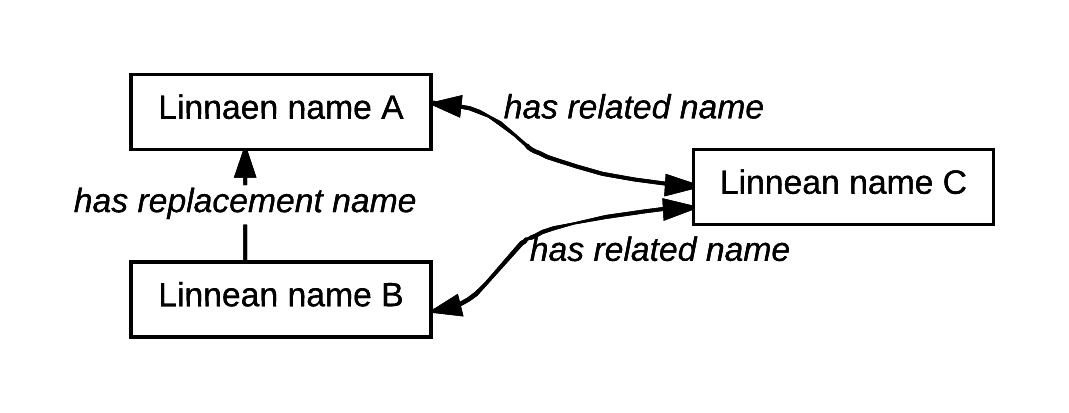
\includegraphics[width=\textwidth]{Figures/scientific-name-patterns}
  \decoRule
  \caption[Scientific name patterns diagram.]{
  Веригите на \emph {заместващи имена} могат да бъдат проследени, за да се намери използваното понастоящем име. \emph{Свързано име} показва, че две имена са свързани по някакъв начин, но не кой е предпочитан.}
  \label{scientific-name-patterns}
\end{figure}

Другият модел е този на \emph{свързани имена} (\cl{relatedName}). Това е по-широк модел, който показва, че две имена са някак си свързани. Например, те могат да бъдат синоними, едното да замества другото, или да сочат към таксономично свързани таксономични понятия. Например, \emph{Harmonia manillana} (\cite{mulsant_monographie_1866}) е свързано с \emph{Caria manillana} \cite {mulsant_monographie_1866} \emph{Harmonia manillana} (според \cite{poorani_harmonia_2016} лектотипус на \emph{Harmonia manillana} (\cite{mulsant_monographie_1866}) sec. \cite{poorani_harmonia_2016} носи името \emph{Caria manillana} \cite{mulsant_monographie_1866}).

\subsubsection{Семантика и употреба}

Както се вижда от фиг.~\ref{taxonomic-name-class-hierarchy-diagram}, таксономичните имена на OpenBiodiv-O са приравнени към NOMEN имена. Илюстрации в примера на Фиг.~\ref{example-taxonomic-name-usage}.

\begin{figure}[h!]
\centering
  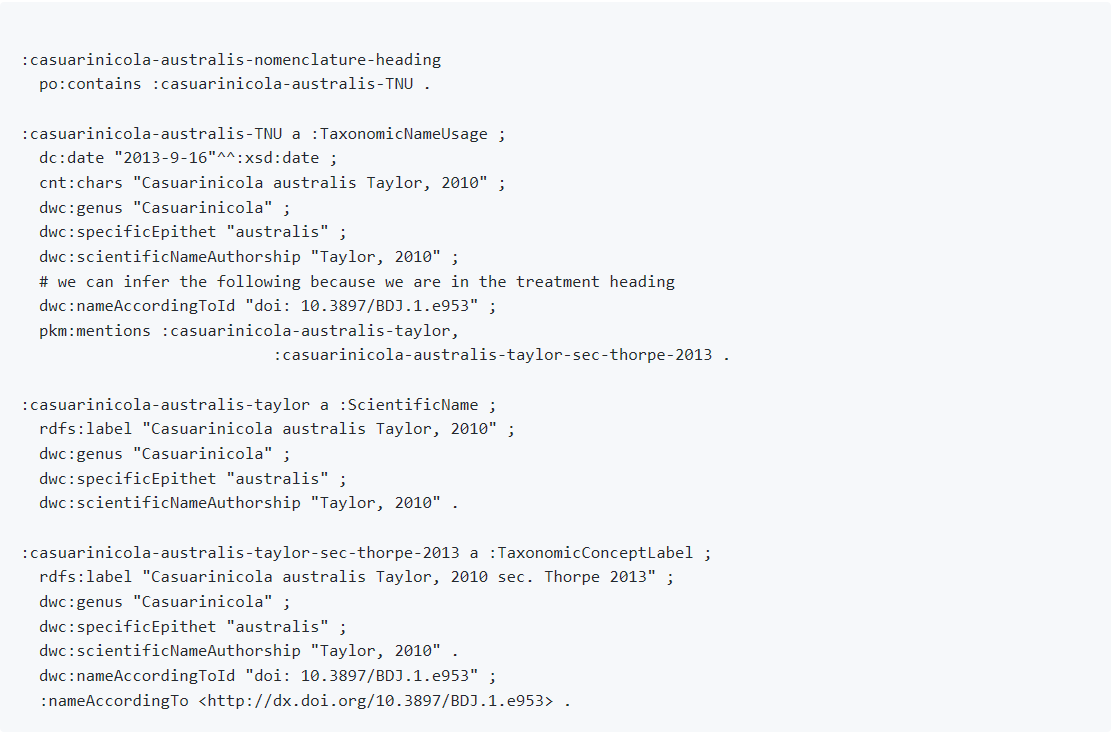
\includegraphics[width=\textwidth]{Figures/example-taxonomic-name-usage}
  \decoRule
  \caption[Example taxonomic name usage.]{
  Тези примери показват как таксономичните имена използват свързващите компоненти на документа.}
  \label{example-taxonomic-name-usage}
\end{figure}

\subsection{Семантично моделиране на таксономичните концепции}

В таксономичните имена на OpenBiodiv-O не са носители на семантична информация за таксоните. Тази задача се изпълнява от нов клас, Taxonomic Concept (\cl{TaxonomicConcept}). Таксономична концепция е теорията, която таксономът формира около таксон посредством научна таксономична публикация. Тя винаги има етикет, състоящ се от таксономичното име и библиографско позоваване на статията, в която името е описано. Въвеждаме и по-общ клас, оперативно таксономично звено (\cl{OperationalTaxonomicUnit}), което може да се използва за всички видове таксономични хипотези, включително такива, които нямат правилен таксономичен етикет . Класовата йерархия е илюстрирана на Фиг.~\ref{taxonomic-concept-diagram}.

\begin{figure}[h!]
\centering
  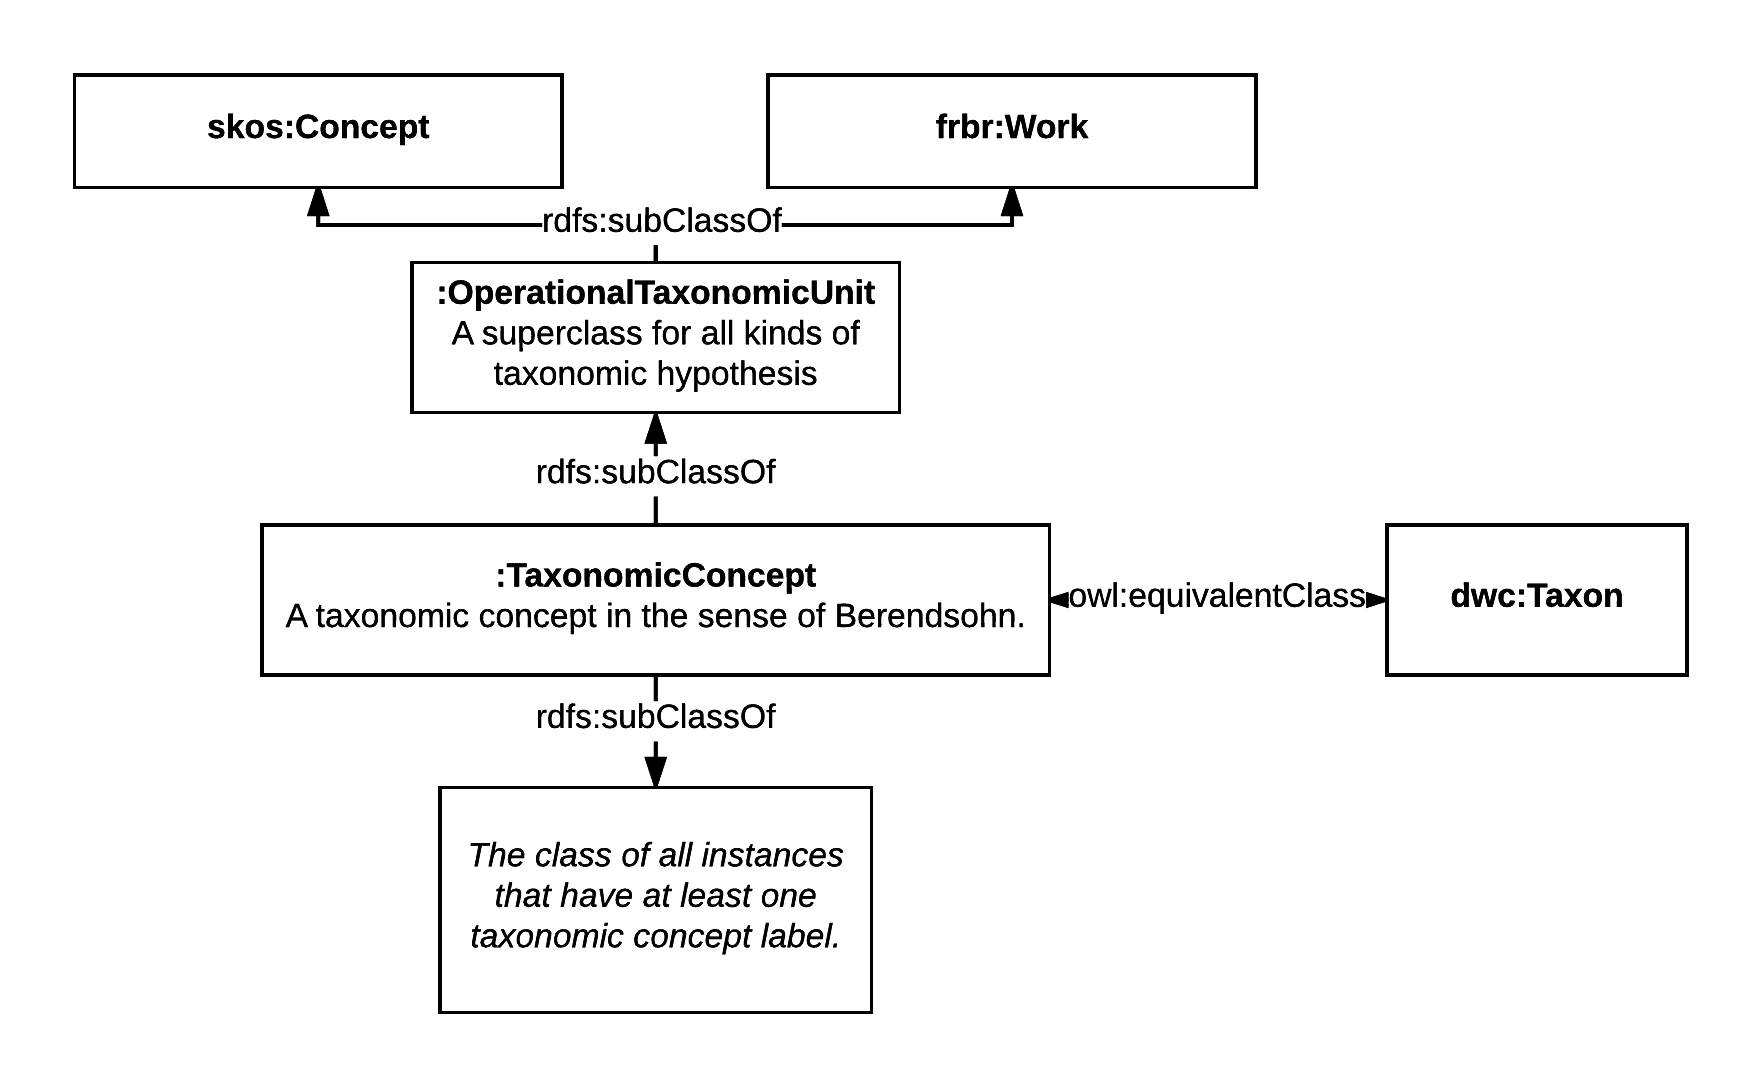
\includegraphics[width=\textwidth]{Figures/taxonomic-concept-diagram}
  \decoRule
  \caption[Taxonomic concept diagram.]{
  Таксономичната концепция е от клас \cl{skos:Concept}, \cl{frbr: Work}, \cl{dwc:Taxon} и има поне един етикет.}
  \label{taxonomic-concept-diagram}
\end{figure}

Свойствата на таксономичните имена са илюстрирани в Фиг.~\ref{name-property-hierarchy}.

\begin{figure}[h!]
\centering
  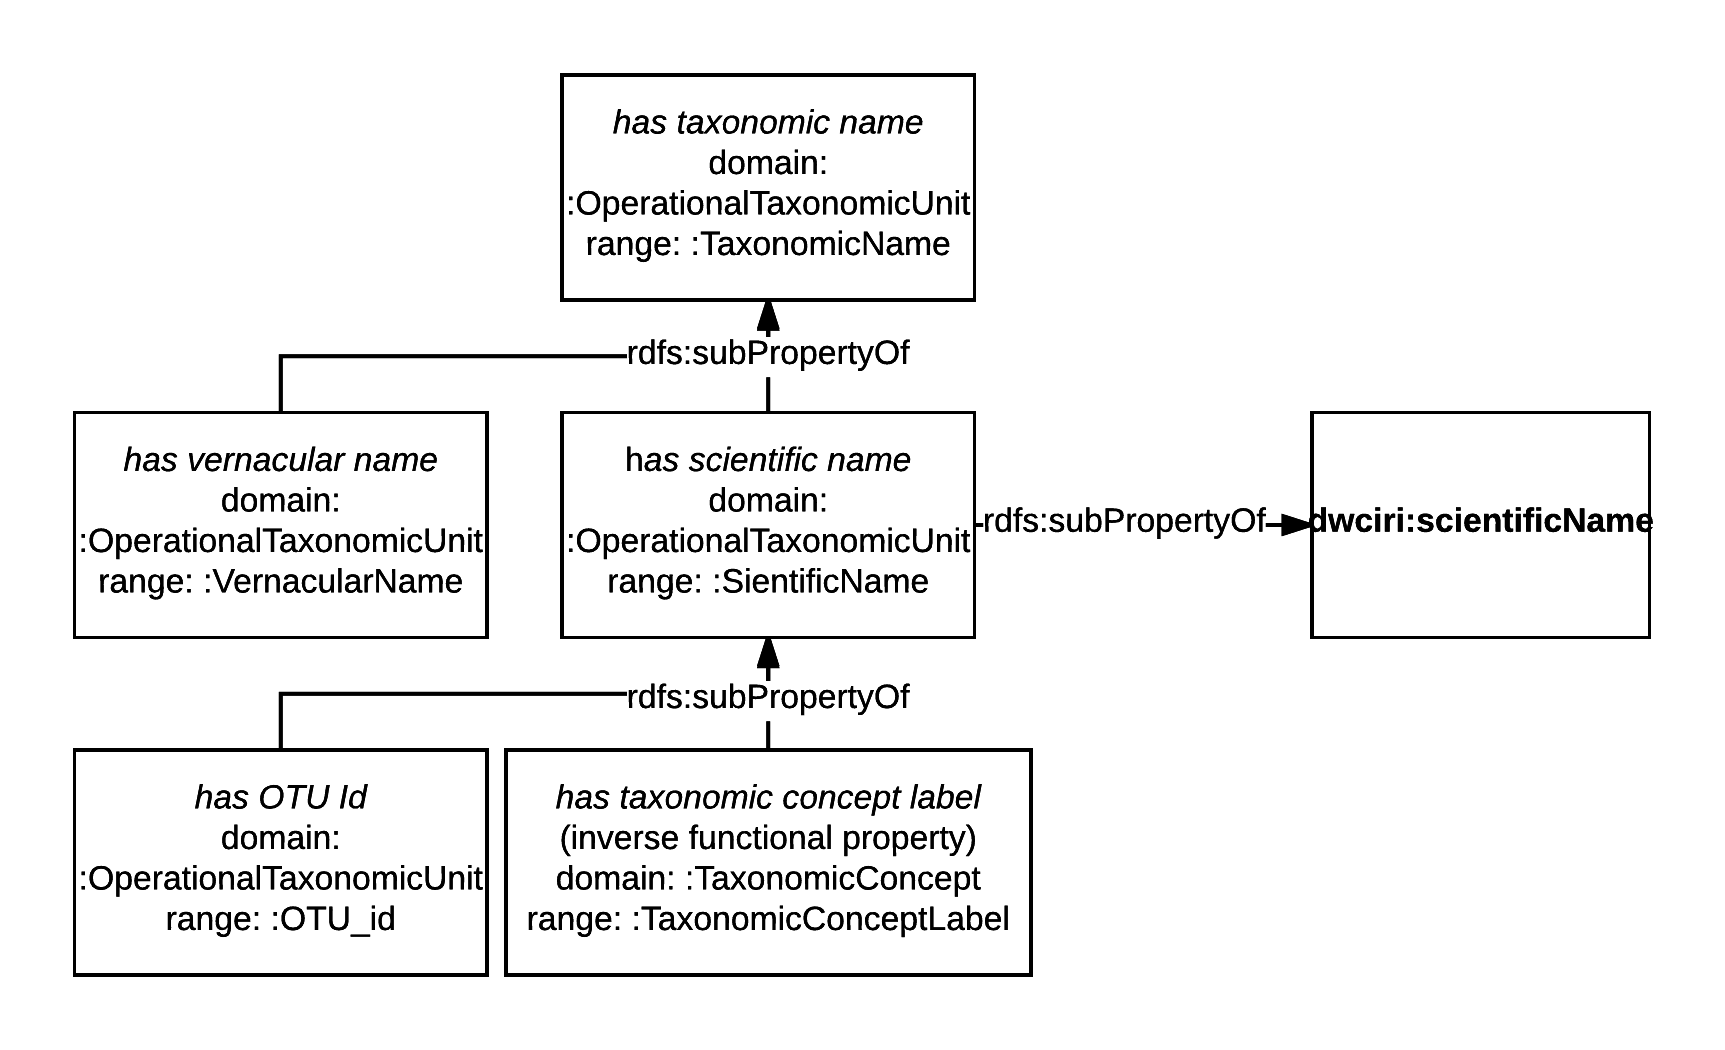
\includegraphics[width=\textwidth]{Figures/name-property-hierarchy}
  \decoRule
  \caption[axonomic name property hierarchy diagram.]
  {Йерархията на свойствата съвпада с йерархията на таксономичните имена и е приравнена към DarwinCore.}
  \label{name-property-hierarchy}
\end{figure}

Двата начина са изразяване на взаимоотношения между таксономични концепции са дадени във Фиг.~\ref{taxonomic-concept-relationships-diagram}).

\begin{figure}[h!]
\centering
  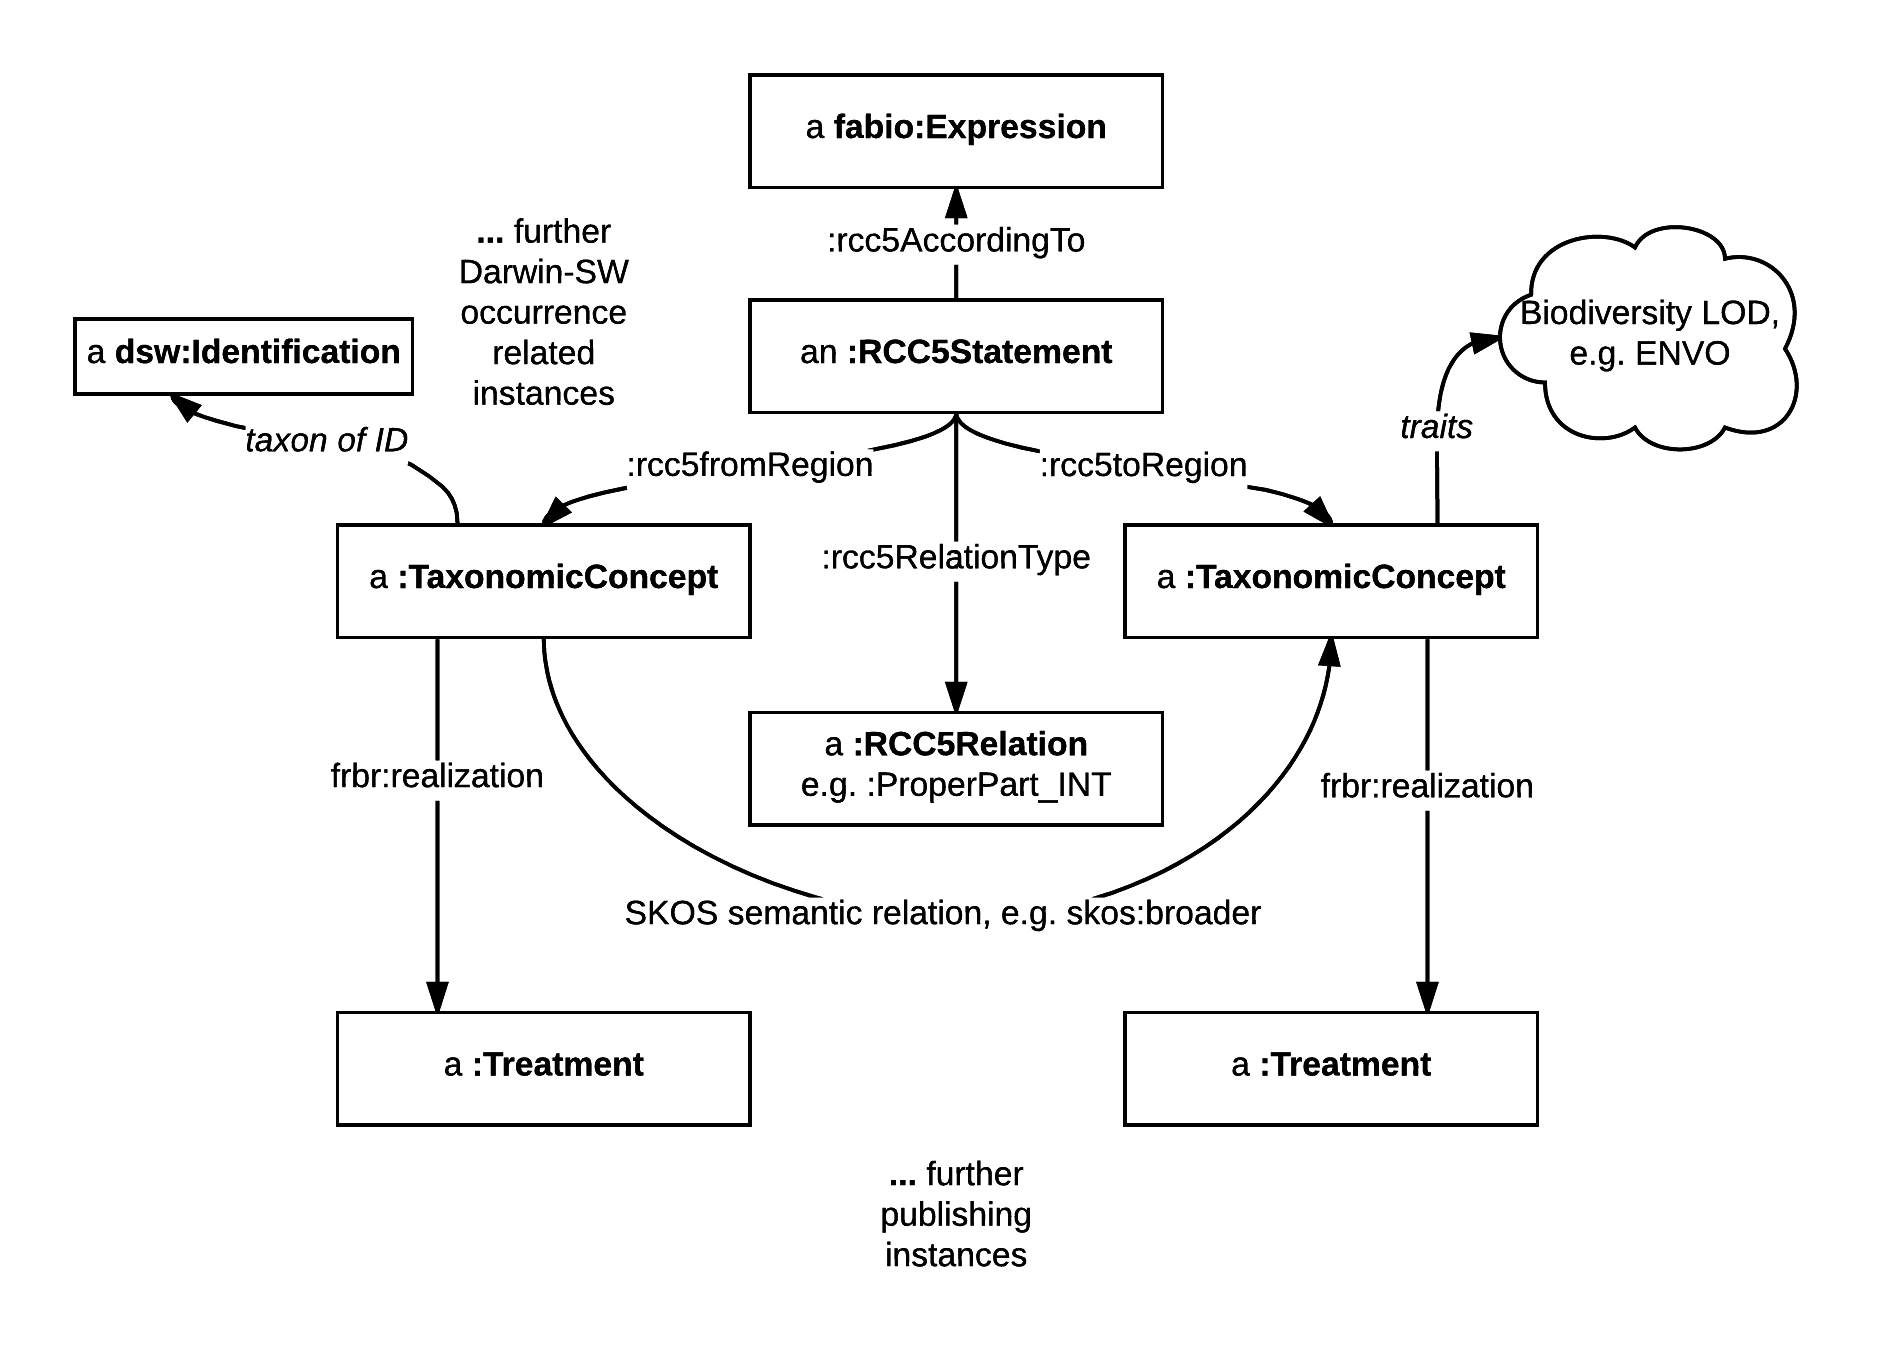
\includegraphics[width=\textwidth]{Figures/taxonomic-concept-relationships-diagram}
  \decoRule
  \caption[Taxonomic concept relationships diagram.]{За да изразите RCC-5 връзка между концепциите, създайте \cl{RCC5Statement} и използвайте съответните свойства, за да свържете две таксономични концепции през него. Освен това, таксономичните понятия са свързани със качества (например екология в ENVO), събития (например Darwin-SW) и са абстрактният клас на Таксономичните дискусии.}
  \label{taxonomic-concept-relationships-diagram}
\end{figure}

Простите отношения не са подходящи за машинен извод. Ето защо \cite{franz_perspectives:_2009}, позовавайки се на \cite{koperski_referenzliste_2000} предложиха да използваме езика RCC-5, за да изразим взаимоотношенията между таксономичните понятия. Тяхни колеги разработиха програмата Euler (\cite{chen_euler/x:_2014}), която използва Answer Set Programming (ASP) за разсъждения и извод по таксономичните взаимоотношения, стъпвайки на RCC-5. Изводната машина за RCC-5 не е част от OpenBiodiv, тъй като тази задача може да бъде изпълнена от Ойлер; въпреки това, ние предоставихме RCC-5 терминилогичен речник. Вж. Фиг.~\ref{example-rcc5-taxonomic-concept-relationships}.

\subsubsection{Семантика и приравняване}

В тази секция таксономичните понятия са приведени в съответствие с DarwinCore (DwC) и е проведена дискусия за това как са представени таксономичните понятия, свързани както с прости отношения (SKOS), така и в подходящ за извод вид (RCC-5). Също така се обсъждат взаимоотношенията между биологичните имена и таксономичните концепции.

\subsubsection{Употреба} Фиг.~ \ref{example-simple-taxonomic-concept-relationships}, Фиг.~\ref{example-rcc5-taxonomic-concept-relationships}, и Фиг.~\ref{example-envo}, и  Fig~\ref{example-treatment-concept}.

\begin{figure}[h!]
\centering
  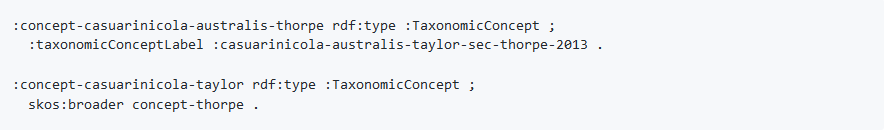
\includegraphics[width=\textwidth]{Figures/example-simple-taxonomic-concept-relationships}
  \decoRule
  \caption[Example simple taxonomic concept relationships.]
  {Можем да използваме семантичните свойства на SKOS, за да илюстрираме прости отношения между таксономичните концепции.}
  \label{example-simple-taxonomic-concept-relationships}
\end{figure}

\begin{figure}[h!]
\centering
  
\includegraphics[width=\textwidth]{Figures/example-rcc5-taxonomic-concept-relationships}
  \decoRule
  \caption[Example of RCC-5 taxonomic concept relationships.]{За да се изрази една RCC-5 връзка между концепциите, създайте \cl{RCC5Sgtatement} и използвайте съответните свойства, за да свържете две таксономични концепции през него.}
  \label{example-rcc5-taxonomic-concept-relationships}
\end{figure}


\begin{figure}[h!]
\centering
  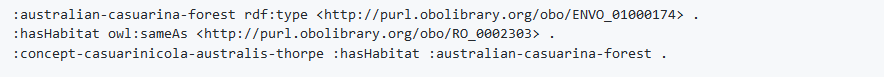
\includegraphics[width=\textwidth]{Figures/example-envo.png}
  \decoRule
  \caption[Example of combining ENVO with OpenBiodiv-O.]{Илюстрация на приравняване към ENVO.}
  \label{example-envo}
\end{figure}



\begin{figure}[h!]
\centering
  
\includegraphics[width=\textwidth]{Figures/example-treatment-concept}
  \decoRule
  \caption[Example connection between a treatment and a taxonomic concept.]{Таксономичната дискусия е реализация/израз/запис на таксономична концепция.}
  \label{example-treatment-concept}
\end{figure}

\section{Дискусия}

Обсъжда се как OpenBiodiv-O е първият по рода си опит да се моделира онтологично таксономичната публикация. Тя проправя пътя към създаване на граф от знания за биологичното разнообразие.

\section{Заключение}

Главата предоставя концептуализация на таксономичния процес и формализация в OpenBiodiv-O. Въвеждат се класове и свойства в областта на публикуването на биоразнообразие и биологичната систематика и ги привежда в съответствие с важните онтологии, специфични за този домейн.
\chapter{Резюме на глава 3: Свързани отворени данни}
\label{chapter-lod}

В глава~\ref{chapter-lod} разглеждаме подробно източниците на данни и техните модели. Създадохме свързани отворени данни OpenBiodiv LOD, съдържащи информация за биологичното разнообразие, извлечена от списанията на Пенсофт, базата данни на Плаци, които е интегрирана с помощта на таксономичния гръбнак на GBIF. Като онтология използваме новия \mbox{OpenBiodiv-O}, разработен в хода на дисертацията. Предлагаме на общността на информатиката за биоразнообразието да използва OpenBiodiv LOD като централна точка на семантичния граф за знания за биоразнообразието. OpenBiodiv LOD е достъпен под \url{http://graph.openbiodiv.net}.

OpenBiodiv LOD е синтетичен набор от данни. Той не съдържа предварително непубликувани данни. Вместо това той интегрира в една база от знания информация, която преди това е била оповестена в академични списания и бази данни. Интеграцията, разбира се, позволява материализацията на скрити взаимоотношения. В следващите няколко параграфа ще обсъдим източниците на информация, които бяха комбинирани от OpenBiodiv LOD и видовете ресурси, които бяха извлечени, както и общия модел на данните. Също така обсъждаме принципите на Linked Open Data, които свързват всичко заедно. Главата завършва с много примери за заявки в набора от данни и с техническа дискусия за начина, по който тя е генерирана.

\section{Източници на данни}

Данните в OpenBiodiv към времето на писането на дисертацията идват от три основни източника: таксономичния гръбнак на GBIF (\cite{gbif_secretariat_gbif_2017}), и научни статии публикувани от Пенсофт, както и съхранявани от Плаци(Fig.~\ref{fig:openbiodiv-sources-simple}).

\begin{figure}
\centering
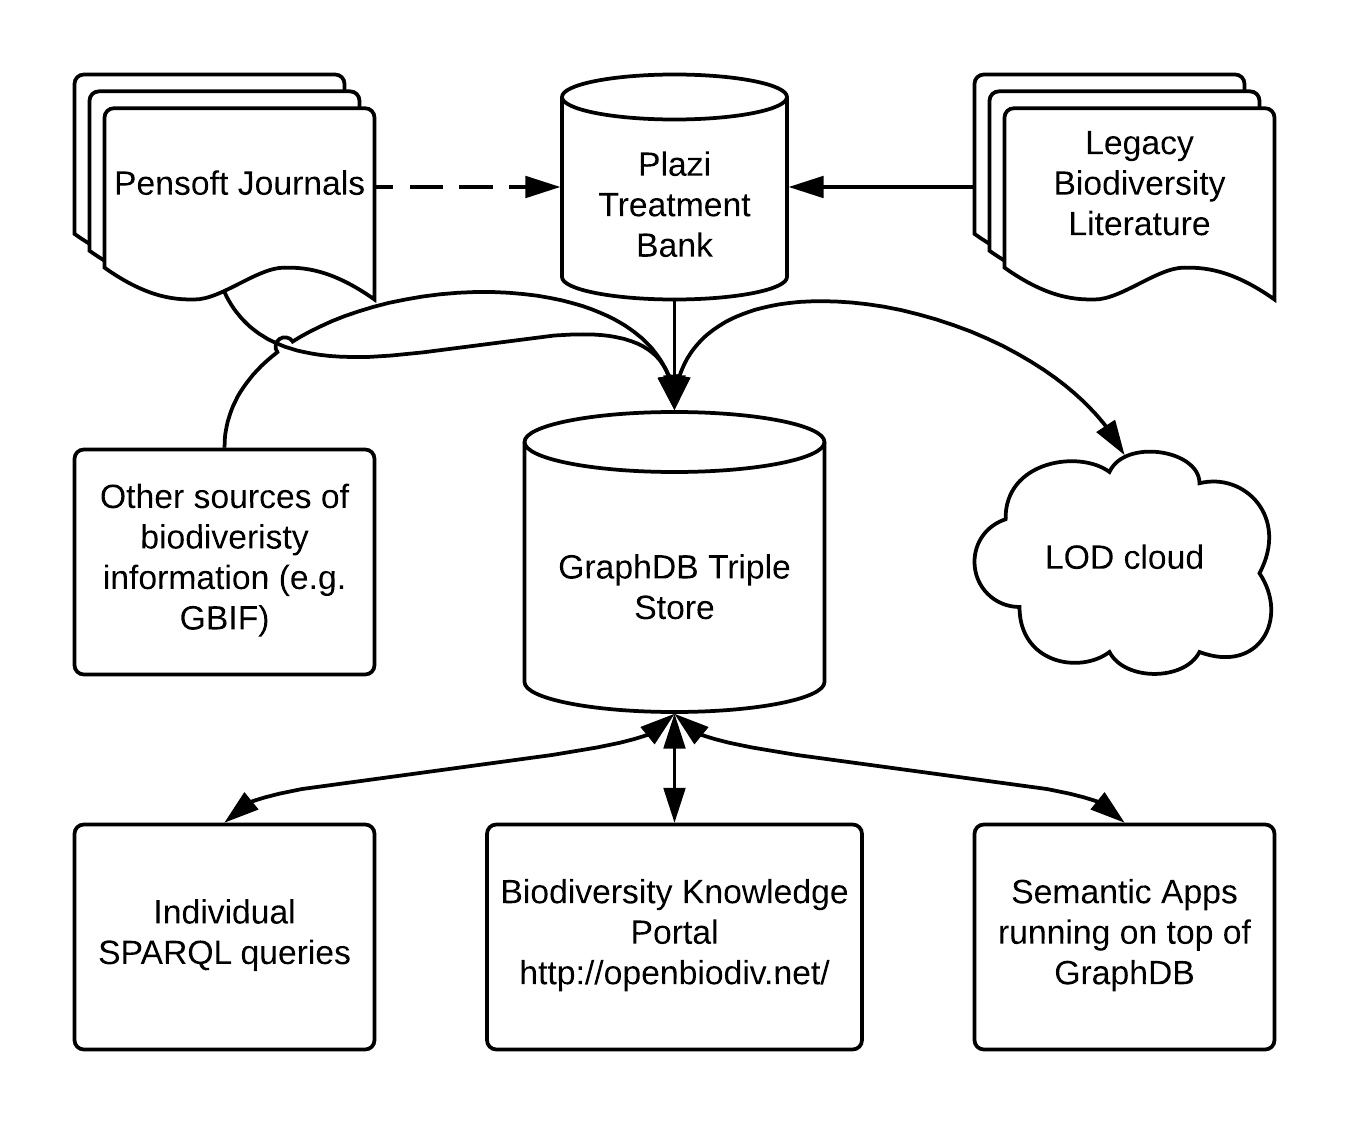
\includegraphics[width=\textwidth]{Figures/openbiodiv-sources-simple}
\decoRule
\caption{Опростен модел на архитектурата на OpenBiodiv от глава~\ref{chapter-openbiodiv} фокусираща върху източниците на информация.}
\label{fig:openbiodiv-sources-simple}
\end{figure}


\subsection{Таксономичен гръбнак на GBIF}

GBIF е най-голямото международно хранилище на данни за наблюдения на организми (occurrence data). GBIF позволява на потребителите да търсят в тяхната система, като използват таксономична йерархия. Например, възможно е да се търсят в базата наблюдения на организми, принадлежащи към определен род: напр. търсене на бръмбар {\textit Harmonia} sec. \cite{gbif_secretariat_gbif_2017} на 30 юни 2018 г. върна 575,376 резултата. Това търсене е възможно благодарение на таксономичния гръбнак на GBIF, Nub (\cite{gbif_secretariat_gbif_2017}). Nub е база данни, която организира таксономични концепции в йерархия, обхващаща всички имена, събрани от GBIF. Тя е синтетична (алгоритмично генерирана) класификация покриваща всички имена, присъстващи в наборите от данни на GBIF. По този начин гръбнакът GBIF не представлява експертен консенсус за това как таксоните са йерархично подредени според еволюционните критерии в природата.

За да предоставим същите възможности на OpenBiodiv, ние  импортирахме Nub като \cl{openbiodiv:TaxonomicConcept} по OpenBiodiv-O (фиг.~\ref {fig:harmonia-halii-visual}).
\begin{figure}
\centering
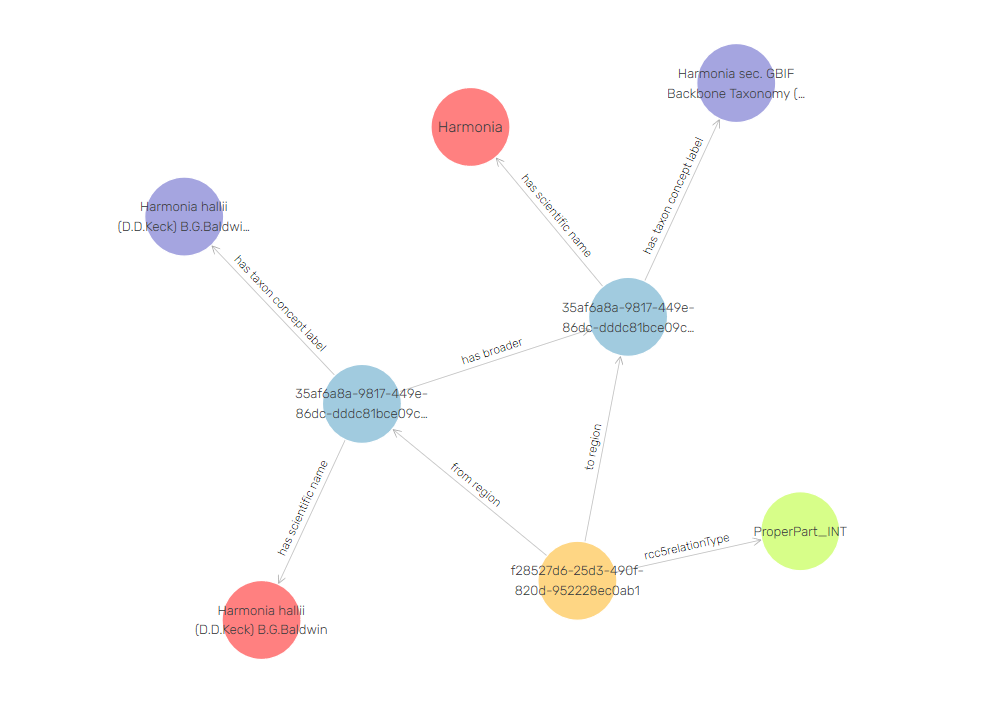
\includegraphics[width=\textwidth]{Figures/harmonia-halii-visgraph}
\decoRule
\caption[Visual graph of \emph{Harmonia halii}]{Илюстрация на представянето на йерархична информаци, импортирана от GBIF като таксономични концепции в OpenBiodiv.}
\label{fig:harmonia-halii-visual}
\end{figure}


\subsection{Пенсфот и Плаци}

Всички валидни статии, от таксономичните списания, публикувани  от Пенсофт и упоменати в Таблица~\ref{rdf-pensoft-journals} бяха конвертирани в RDF и съхранени в гр\'{а}фа от знания на биологичното разнообразие. В допълнение, всички валидни таксономични дискусии (treatments) на Плаци бяха конвертирани в RDF и също съхранени в гр\'{а}фа. Процедурата по RDF-изиране се повтаря всяка седмица и по този начин семантичната база данни винаги съдържа най-новите статии и таксономични дискусии. RDF-изацията е възможнa благодарение на факта, че списанията на Пенсофт публикуват статии в TaxPub XML (\cite{catapano_taxpub:_2010}) докато Плаци публикува дискусиите си в TaxonX (\cite{penev_xml_2011}) (Fig.~\ref{fig:tnu-vis}). И двете схеми са стандартни и общо-достъпни.

\begin{table}[h!]
\caption{Списания ма Пенсофт, които са превърнати в RDF.}
      \begin{tabular}{ccc}
        \hline
          Journal Name             & Submission Style & Number of Articles\\  \hline
          ZooKeys                 & Word document & 3829\\
          PhytoKeys               & Word document & 537\\
          MycoKeys                & Word document & 127\\
          Biodiversity Data Journal & Web based (ARPHA) & 490\\
          Journal of Orthoptera Research & Word document & 32
      \end{tabular}
      \label{rdf-pensoft-journals}
\end{table}

\begin{table}[h!]
\caption{Типове данни, маркирани в TaxPub and TaxonX и тяхната кореспондеция към RDF типовете, които се използват в OpenBiodiv.}
      \begin{tabular}{cccc}
        \hline
          Datatype             & TaxPub & TaxonX & RDF Type\\  \hline
          Article metadata     & T & T & {\tt fabio:JournalArticle} and related\\
          Keyword group        & T & F & {\tt openbiodiv:KeywordGroup} \\
          Abstract             & T & T & {\tt sro:Abstract}\\
          Title                & T & F & {\tt doco:Title} \\
          Author               & T & T & {\tt foaf:Person} \\
          Introduction section & T & F & {\tt deo:Introduction}\\
          Discussion section   & T & T & {\tt orb:Discussion}\\
          Treatment section    & T & T & {\tt openbiodiv:Treatment}\\
          Nomenclature section & T & T & {\tt openbiodiv:NomenclatureSection}\\
          Materials examined   & T & T & {\tt openbiodiv:MaterialsExamined}\\
          Diagnosis section    & T & T & {\tt openbiodiv:DiagnosisSection} \\
          Distribution section & T & T & {\tt openbiodiv:DistributionSection}\\
          Taxonomic key        & T & T & {\tt openbiodiv:TaxonomicKey}\\
          Figure               & T & T & {\tt doco:Figure}\\
          Taxonomic name usage & T & T & {\tt openbiodiv:TaxonomicNameUsage}
      \end{tabular}
      \label{datatypes-taxpub-taxonx}
\end{table}

\begin{figure}
\centering
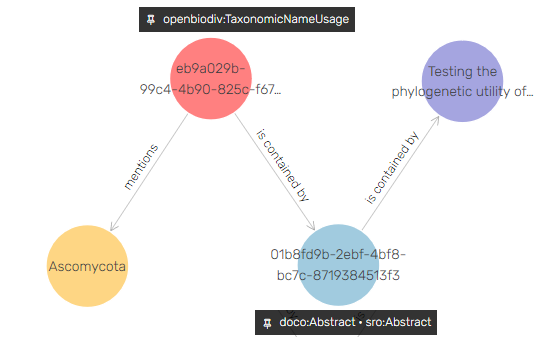
\includegraphics[width=\textwidth]{Figures/tnu-vis}
\decoRule
\caption[Visual graph of a taxonomic name usage]{Употреба на таксономични имена в OpenBiodiv (taxonomic name usage).}
\label{fig:tnu-vis}
\end{figure}

\section{Свързани отворени данни}

Linked Open Data (LOD, \cite{heath_linked_2011}) е идея на Семантичната Мрежа (\cite{berners-lee_semantic_2001}) целяща да гарантира полезността на данни публикувани в Мрежата, като улеснява тяхното повторно намиране и употреба от трети лица. В тази секция разясняваме принципите на Свързаните Отворени Данни и тяхното приложение в OpenBiodiv (\cite{heath_linked_2011}).

\begin{figure}
\centering
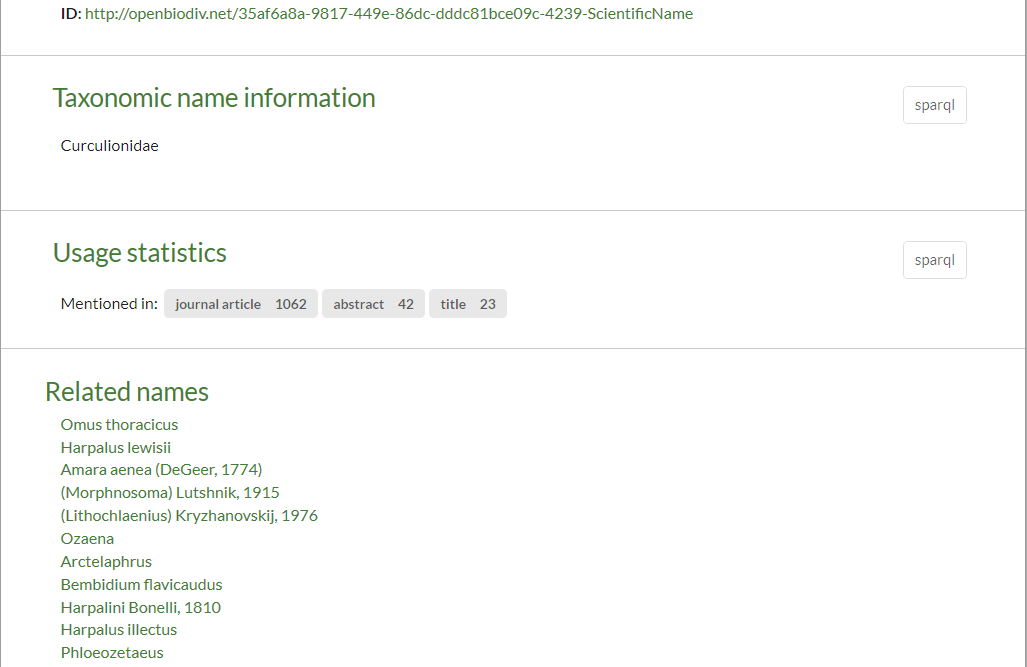
\includegraphics[width=\textwidth]{Figures/portal-name-visualization}
\decoRule
\caption{Визуализация.}
\label{fig:portal-name-visualization}
\end{figure}


\section{Модел на данните}

Подчертаваме, че използваме модела подробно разяснен в глава~\ref{chapter-ontology} и допълнителните онтологии (Fig.~\ref{fig:community-ontologies}).

\begin{figure}
\centering
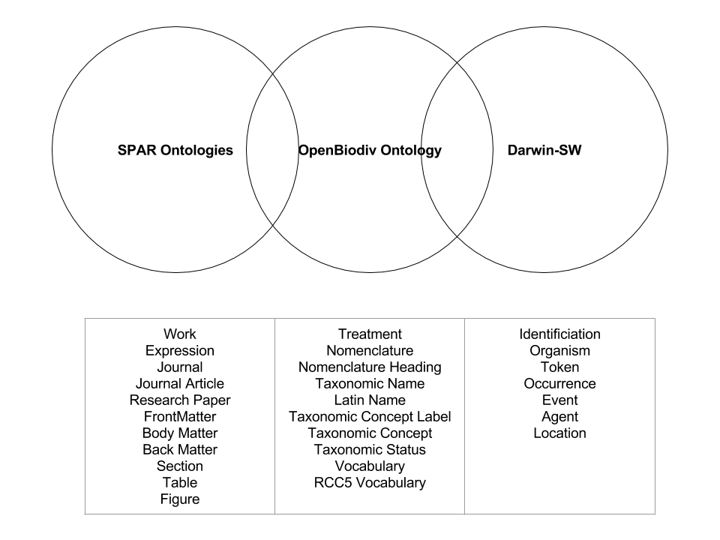
\includegraphics[width=\textwidth]{Figures/community-ontologies}
\decoRule
\caption[Overlap of OpenBiodiv-O with Community Ontologies]{Връзка между OpenBiodiv-O и други публично-достъпни онтологии.}
\label{fig:community-ontologies}
\end{figure}

\section{Примерен SPARQL}

В тази секция илюстрираме, как представеният модел за данни, заедно с инкорпорираната в базата данни информация е достатъчен за да изпълним някои много интересни заявки върху графа за знания.

\subsection{Прости заявки}

В тази подскекция даваме прости заявки. Напр. как да търсим по автори, по научни имена и т.н.

\subsubsection{Заявка върху структурата на статията} 

Тъй като в OpenBiodiv LOD статиите са разбити по техните компоненти (вж напр. Таблица~\ref{datatypes-taxpub-taxonx}) и споменаванията на таксони (taxonomic name usages) винаги са свързани със специфична част на статията, може да правим запитвания, използващи тази структура.

\subsubsection{Запитване за таксономични концепции}

Дадени са пример за SPARQL заявки, базиращи се на таксономични концепции.

\subsubsection{Размито търсене с Lucene}

Използваме Lucene connector (\cite{ontotext_graphdb_2018}) на GraphDB, за да допълним точните търсения с размити търсения, където се допускат правописни грешки.

\subsection{Отговаряне на експертни въпроси}

Поради машината си за извод, OpenBiodiv може да функционира като експертна система. В тази подсекция даваме примери за такова запитване.

\subsubsection{Проверка на валидността на таксономично име}

Проверяваме, дали дадено таксономично име е валидно, т.е. е уместно да се употребява в научен контекст, или е било прехамахнато или заменено от друго име.

\subsubsection{Оценка на научната загуба след пожара в Museu Nacional в Бразилия}

Може да запитаме експертната система OpenBiodiv да даде списък с видовете, чиито екземпляри бяха загубени в пожара в Рио де Жанейро.

\section{Как създадохме данните?}

В тази секция се разкриват техническите подробности за това, как данните бяха създадени.

\subsection{Получаване на данни}

Дават се адресите в Интернет, където данните в суров вид могат да бъдат достъпвани.

\subsection{Инструменти}

Използват се следните инструменти

\begin{enumerate}
\item{Пакет RDF4R}
\item{Пакет ROpenBio}
\item{Пакет TSV4RDF разработен от Пенсофт}
\item{Базисен код на OpenBiodiv}
\end{enumerate}

\subsection{Трансформация от XML в RDF}

Използваме йерархичната структура на XML, за да решим проблема рекурсивно с помощта на следния Extractor, документиран в Алгоритъм~\ref{algo:extractor}.

% http://tug.ctan.org/macros/latex/contrib/algorithmicx/algorithmicx.pdf
\begin{algorithm}
\caption{Екстрактор}
\begin{algorithmic}[1]
\Procedure {Extractor}{XML Node $X$}
\State $a \leftarrow$ extract atoms of $X$
\Comment Atoms extraction
\State $r \leftarrow$ construct RDF from $a$
\Comment RDF construction
\State $C \leftarrow$ find relevant sub-nodes of $X$
\Comment Recursively applies itself
\State $R \leftarrow$ apply Extractor on each $C_i \in C$
\State \Return $r \bigcup R$
\EndProcedure
\end{algorithmic}
\label{algo:extractor}
\end{algorithm}

\subsubsection{Извличане на атомите}

Текстовите полета в XML ще наричаме атоми. Тяхното извличане се осъществява с помощта на езика XPATH. Тук разясняваме, как става това.

\subsubsection{Генериране на RDF}

След извичане на атомите, те могат да бъдат събрани обратно във формата на RDF. 

\subsubsection{Стратегия разделяй и владей}

Проблемът за RDF-изиранато на цял XML файл е реализиран посредством разбиването му на малки проблеми, за които решението е тривиално като в горния пример за RDF-изирането на даден автор или на метаданните на дадена статия.

\subsubsection{Дефиниране на трансформацията}

За да работи Extractor, трябва да дефинираме XML схемата. Спецификацията включва какви XML възли търсим и къде се намират. След това рекурсивно се указва за всеки възел кои под-възли търсим и тяхното местоположение на XPATH спрямо техния родителски възел. И накрая, за всеки възел трябва да дадем атомните места и да напишем конструктор. Спецификацията на трансформацията се извършва в R6 калс на R. Определихме две схеми, които споделят същите конструктори: TaxPub\footnote{\url{https://github.com/pensoft/ropenbio/blob/redesign/R/taxpub.R}} и TaxonX\footnote{\url{https://github.com/pensoft/ropenbio/blob/redesign/R/taxonx.R}}.

\subsection{Качване в базата данни и допълнителна обработка}

Извлечените RDF твърдения се изпращат в GraphDB, който се намира на адрес \url{http://graph.openbiodiv.net/}. Освен материлизирани твърдения по онтологията, след всеки ъпдейт, изпълняваме следните допълни правила: 

\subsubsection{Ъпдейт на заместващите имена}

Изгражда връзките от тип \cl{replacementName} между вмъкнатите имена.

\section{Дискусия}

Установихме, че обемът данни, който обработване в комбинация с пълна OWL логика води до неприемлива производителност. В тази секция разглеждаме този проблем (Фиг.~\ref{fig:statements-report}).

\begin{figure}
\centering
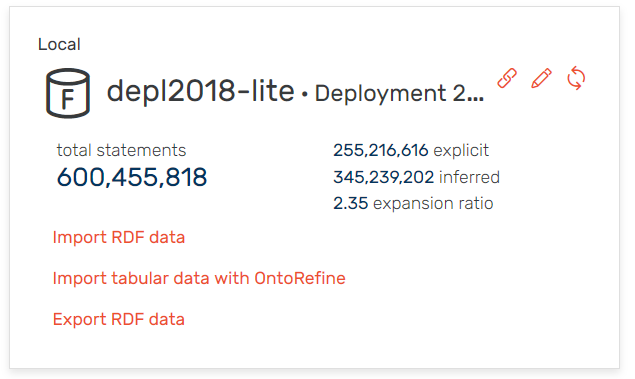
\includegraphics[width=\textwidth]{Figures/active-repository}
\decoRule
\caption[Statements report]{Брой твърдения.}
\label{fig:statements-report}
\end{figure}

\begin{figure}
\centering
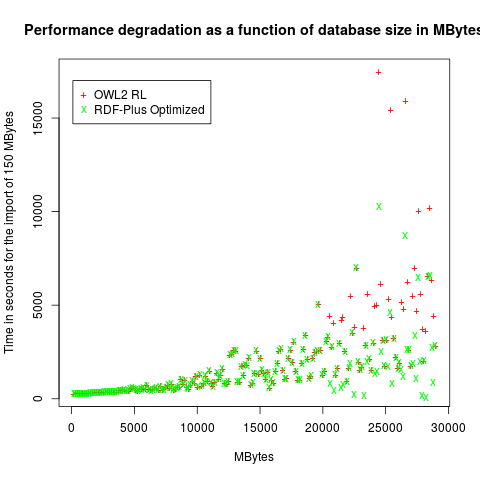
\includegraphics[width=\textwidth]{Figures/performance-degradation-both}
\decoRule
\caption[Performance degradation]{Визуализация на деградацията на производителността.}
\label{fig:performance-degradation}
\end{figure}

Правим някои основни изводи и очертаваме насоки за бъдещо развитие.
\chapter{Summary of Chapter 4: An R Library for Working with RDF}
\label{chapter-rdf4r}

RDF4R ({\tt rdf4r}) is an R package for working with Resource Description Framework (\cite{rdf_working_group_resource_2014}) data. It was developed as part of the OpenBiodiv project but is completely free of any OpenBiodiv-specific code and can be used for generic purposes requiring tools to work with RDF data in the R programming environment (\cite{r_core_team_r:_2016}).

\section{Installation}

In this section we describe how to install the RDF4R package. Installation is straighforward and consists of two steps: (1) resolve dependencies and (2) build the package from source using \cl{devtools::install_github}.

\section{Specification}

In this section we present the specifications of RDF4R by detailing the features of the package. Each feature has a dedicated subsection.

\subsection{Connection to a triple-store}

It is possible to establish both basic connections (requiring no password or requiring basic HTTP user-pass authentication) or connection secured with an API access token.

\subsection{Work with repositories on a triple-store}

Once a connection to a triple-store has been established, it is possible to inspect the talk protocol version, view the list of repositories on the database, execute SPARQL Read (SELECT keyword and related) and SPARQL Update (INSERT and related) queries on the database, as well as submit serialized RDF data directly to the database.

\subsection{Function factories to convert SPARQL queries to R functions}

An important feature of RDF4R are its facilities for converting SPARQL queries and the like to R functions.

\subsection{Work with literals and identifiers}

The building blocks of RDF are literals (e.g. strings, numbers, dates, etc.) and resource identifiers. RDF4R provides classes for literals and resource identifiers that are tightly integrated with the other facilities of the package.

\subsection{Prefix management}

Prefixes are managed automatically during serialization by being extracted from the resource identifiers.

\subsection{Creation and serialization of RDF}

The serialization function supports Turtle (and its variant Trig, \cite{bizer_rdf_2014}) and adding new triples.

\begin{lstlisting}[language=SPARQL,
caption=Using brackets to express RDF blank nodes in Turtle/TriG.,
label=fig:turtle-brackets,
basicstyle=\ttfamily\tiny]
@prefix foaf: <http://xmlns.com/foaf/0.1/> .

# :someone knows someone else, who has the name "Bob".
:someone foaf:knows [ foaf:name "Bob" ] .
\end{lstlisting}

\subsection{A basic vocabulary of semantic elements}

RDF4R has some basic resource identifiers for widely used classes and predicates predefined (e.g. for {\tt rdf:type}, {\tt rdfs:label}, etc.).

\section{Usage}

Here, we explain how to use the package RDF4R by means of examples. In order to fully utilize the package capabilities, one needs to have access to an RDF graph database. We have made available a public endpoint (see next paragraph) to allow the users of the package to experiment. Since write access is enabled, please be considerate and don't issue catastrophic commands.

\section{Discussion}

\subsection{Related Packages}

The closest match to RDF4R is the {\tt rdflib} (\cite{boettiger_rdflib:_2018}). The development of the two packages was simultaneous and independent until {\tt rdflib}'s first official release on Dec 10, 2017. This explains why two closely related R packages for working with RDF exist. After the release of {\tt rdflib} work was started  to make both packages compatible with each other. In our opinion, the packages have different design philosophies and are thus complementary.

{\tt rdflib} is a high-level wrapper to {\tt redland} (\cite{jones_redland:_2016}), which is a low-level wrapper to the C {\tt librdf} (\cite{beckett_redland_2014}), a powerful C library that provides support for RDF. {\tt librdf} provides an in-memory storage model for RDF beyond what is available in RDF4R and also persistent storage working with a number of databases. It enables the user to query RDF objects with SPARQL. Thus, {\tt librdf} can be considered a complete graph database implementation in C.

In our opinion, {\tt redland} is more complex than needed for the purposes of OpenBiodiv. By the onset of the OpenBiodiv project it was available\footnote{But not {\tt rdflib}!}; however, we decided not to use it as a decision was made to rely on GraphDB for our storage and querying. Note that RDF4R's main purpose is to provide a convenient R interface for users of GraphDB and similar RDF4J compatible graph databases.

A feature that differentiates {\tt rdflib} from RDF4R is the design philosophy. RDF4R was designed primarily with the Turtle and TriG serializations in mind. This means that RDF4R can work with named graphs, whereas their usage is discouraged or perhaps impossible with {\tt rdflib}\footnote{The issue was discussed on the {\tt librdf} GitHub page, \url{https://github.com/ropensci/rdflib/issues/23}.}, even though {\tt rdflib}'s default format is N-Quads.

Another differentiating feature between RDF4R and {\tt rdflib} is that RDF4R provides facilities for converting SPARQL and related statements to native R functions!

In a future release of RDF4R (2.0) we would like to replace or extend its in-memory model with {\tt rdflib}'s. This is why we would like to make the packages fully compatible and have contributed several patches to {\tt rdflib}\footnote{Please, consult the commit history under \url{https://github.com/ropensci/rdflib}.}). Thus, it will be possible for the user of RDF4R to retain its syntax and high-level features--- constructor factories, functors, etc., and the ability to use named graphs---but benefit from performance increases, stability, and scalability with the {\tt redland/rdflib/librdf} backend.

This will enable the users of the R programming environment to use whichever syntax they prefer and benefit from an efficient storage engine.

\subsection{Elements of Functional Programming (FP)}

In this subsection we discuss how patterns from functional programming were used to create RDF4R.

\subsection{Elements of Object-Oriented Programming (OOP)}

In this subsection we discuss how patterns from object-oriented programming were used to create RDF4R.

\chapter{Summary of Chapter 5: Workflows for Biodiversity Data}
\label{chapter-case-study}

In this chapter we discuss two automated workflows for exchange of biodiversity data developed as part of OpenBiodiv: (1) automatic import of specimen records into manuscripts, and (2) automatic generation of data paper manuscripts from Ecological Metadata Language (EML) metadata. The workflows were presented at a webinar for the orgnization iDigBio\footnote{Integrated Digitized Biocollections (iDigBio) is a US-based aggregator of biocollections data. They hold regular webinars and workshops aimed at improving biodiversity informatics knowledge, which are attended by collection managers, scientists, and IT personnel. Thus, doing a presentation for iDigBio was an excellent way of making the research and tools-development efforts of OpenBiodiv widely known and getting feedback from the community.} and published as a paper (\cite{senderov_online_2016}).

The slides from the presentation as well as a PDF of the paper are available from the webinar GitHub page under \url{https://github.com/vsenderov/idigbio-webinar}.

\section{Introduction}

Information on occurrences of species and information on the specimens that are evidence for these occurrences (specimen records) is stored in different biodiversity databases. These databases expose the information via public REST API's. I focused on the Global Biodiversity Information Facility (GBIF), Barcode of Life Data Systems (BOLD), iDigBio, and PlutoF, and utilized their API's to import occurrence or specimen records directly into a manuscript edited in the ARPHA Writing Tool (AWT).

Furthermore, major ecological and biological databases around the world provide information about their datasets in the form of EML. A workflow was developed for creating data paper manuscripts in AWT from EML files. Such files could be downloaded, for example, from GBIF, DataONE, or the Long-Term Ecological Research Network (LTER Network).

The development of these workflows focuses on two areas: optimizing the workflow of specimen data and optimizing the workflow of dataset metadata. These efforts resulted in the functionality that it is now possible, via a record identifier, to directly import specimen record information from the Global Biodiversity Information Facility (GBIF), Barcode of Life Data Systems (BOLD), iDigBio, or PlutoF into manuscripts in the ARPHA Writing Tool (AWT). No manual copying or retyping is required. 

\section{Presentation}

A video recording of the presentation is available\footnote{\url{http://idigbio.adobeconnect.com/p7sg0aym3e3/}}. More information can be found in the webinar information page\footnote{\url{http://www.idigbio.org/content/online-direct-import-specimen-records-idigbio-infrastructure-taxonomic-manuscripts}}. The slides of the presentation are attached as supplementary files and are deposited in Slideshare\footnote{\url{http://www.slideshare.net/ViktorSenderov/online-direct-import-of-specimen-records-from-idigbio-infrastructure-into-taxonomic-manuscripts}}.

During the presentation we conducted a poll about the occupation of the attendees, the results of which are summarized in Fig.~\ref{fig:webinar-poll}. Of the participants who voted, about a half were scientists, mostly biologists, while the remainder were distributed across IT specialists and librarians, with 20\% "Other." The other categories might have been administrators, decision-makers, non-biology scientists, collections personnel, educators, etc.

\begin{figure}
\centering
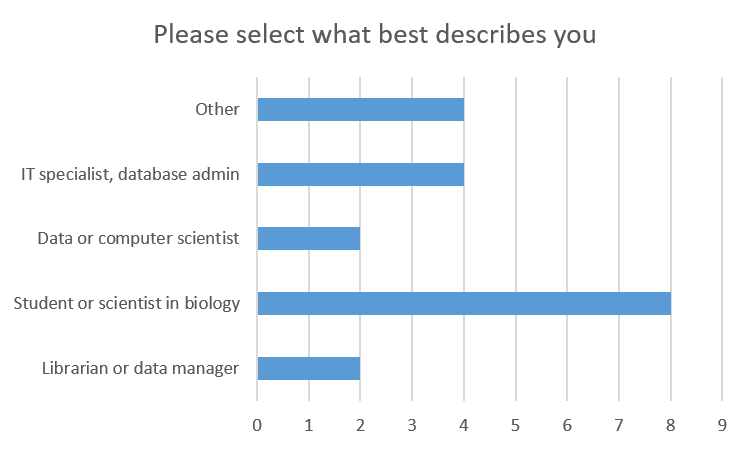
\includegraphics[width=\textwidth]{Figures/webinar-pool}
\decoRule
\caption{Poll results about composition of audience during live participation..}
\label{fig:webinar-poll}
\end{figure}

At the end of the presentation, very interesting questions were raised and discussed. For details, see the ``Results and discussion'' section of this paper.

\section{Methods}

Both workflows discussed  rely on three key standards: RESTful API's for the web (\cite{kurtz_what_2013}), Darwin Core (\cite{wieczorek_darwin_2012}), and EML (\cite{fegraus_maximizing_2005}).

\subsection{Development of workflow 1: Automated specimen record import}

In this subsection we discuss the development of Workflow 1: Automated specimen record import.

\subsection{Development of workflow 2: Automated data paper generation}

In this subsection we discuss the development of Workflow 1: Automated specimen record import.

\section{Results and Discussion}

\subsection{Workflow 1: Automated specimen record import into manuscripts developed in the ARPHA Writing Tool}

It is now possible to directly import a specimen record as a material citation in an ARPHA Taxonomic Paper from GBIF, BOLD, iDigBio, and PlutoF (Slide 5, as well as Fig.~\ref{fig:workflow-idigbio}). The workflow from the user's perspective has been thoroughly described in a blog post; concise stepwise instructions are available via ARPHA's Tips and tricks guidelines. In a nutshell, the process works as follows:

\begin{enumerate}
\item{At one of the supported data portals (BOLD, GBIF, iDigBio, PlutoF), the author locates the specimen record he/she wants to import into the Materials section of a Taxon treatment (available in the Taxonomic Paper manuscript template).}
\item{Depending on the portal, the user finds either the occurrence identfier of the specimen, or a database record identifier of the specimen record, and copies that into the respective upload field of the ARPHA system (Fig.~\ref{fig:occurrence-input-mask}).}
\item{After the user clicks on ``Add,'' a progress bar is displayed, while the specimens are being uploaded as material citations.}
\item{The new material citations are rendered in both human- and machine-readable DwC format in the Materials section of the respective Taxon treatment and can be further edited in AWT, or downloaded from there as a CSV file.}
\end{enumerate}

\begin{figure}
\centering
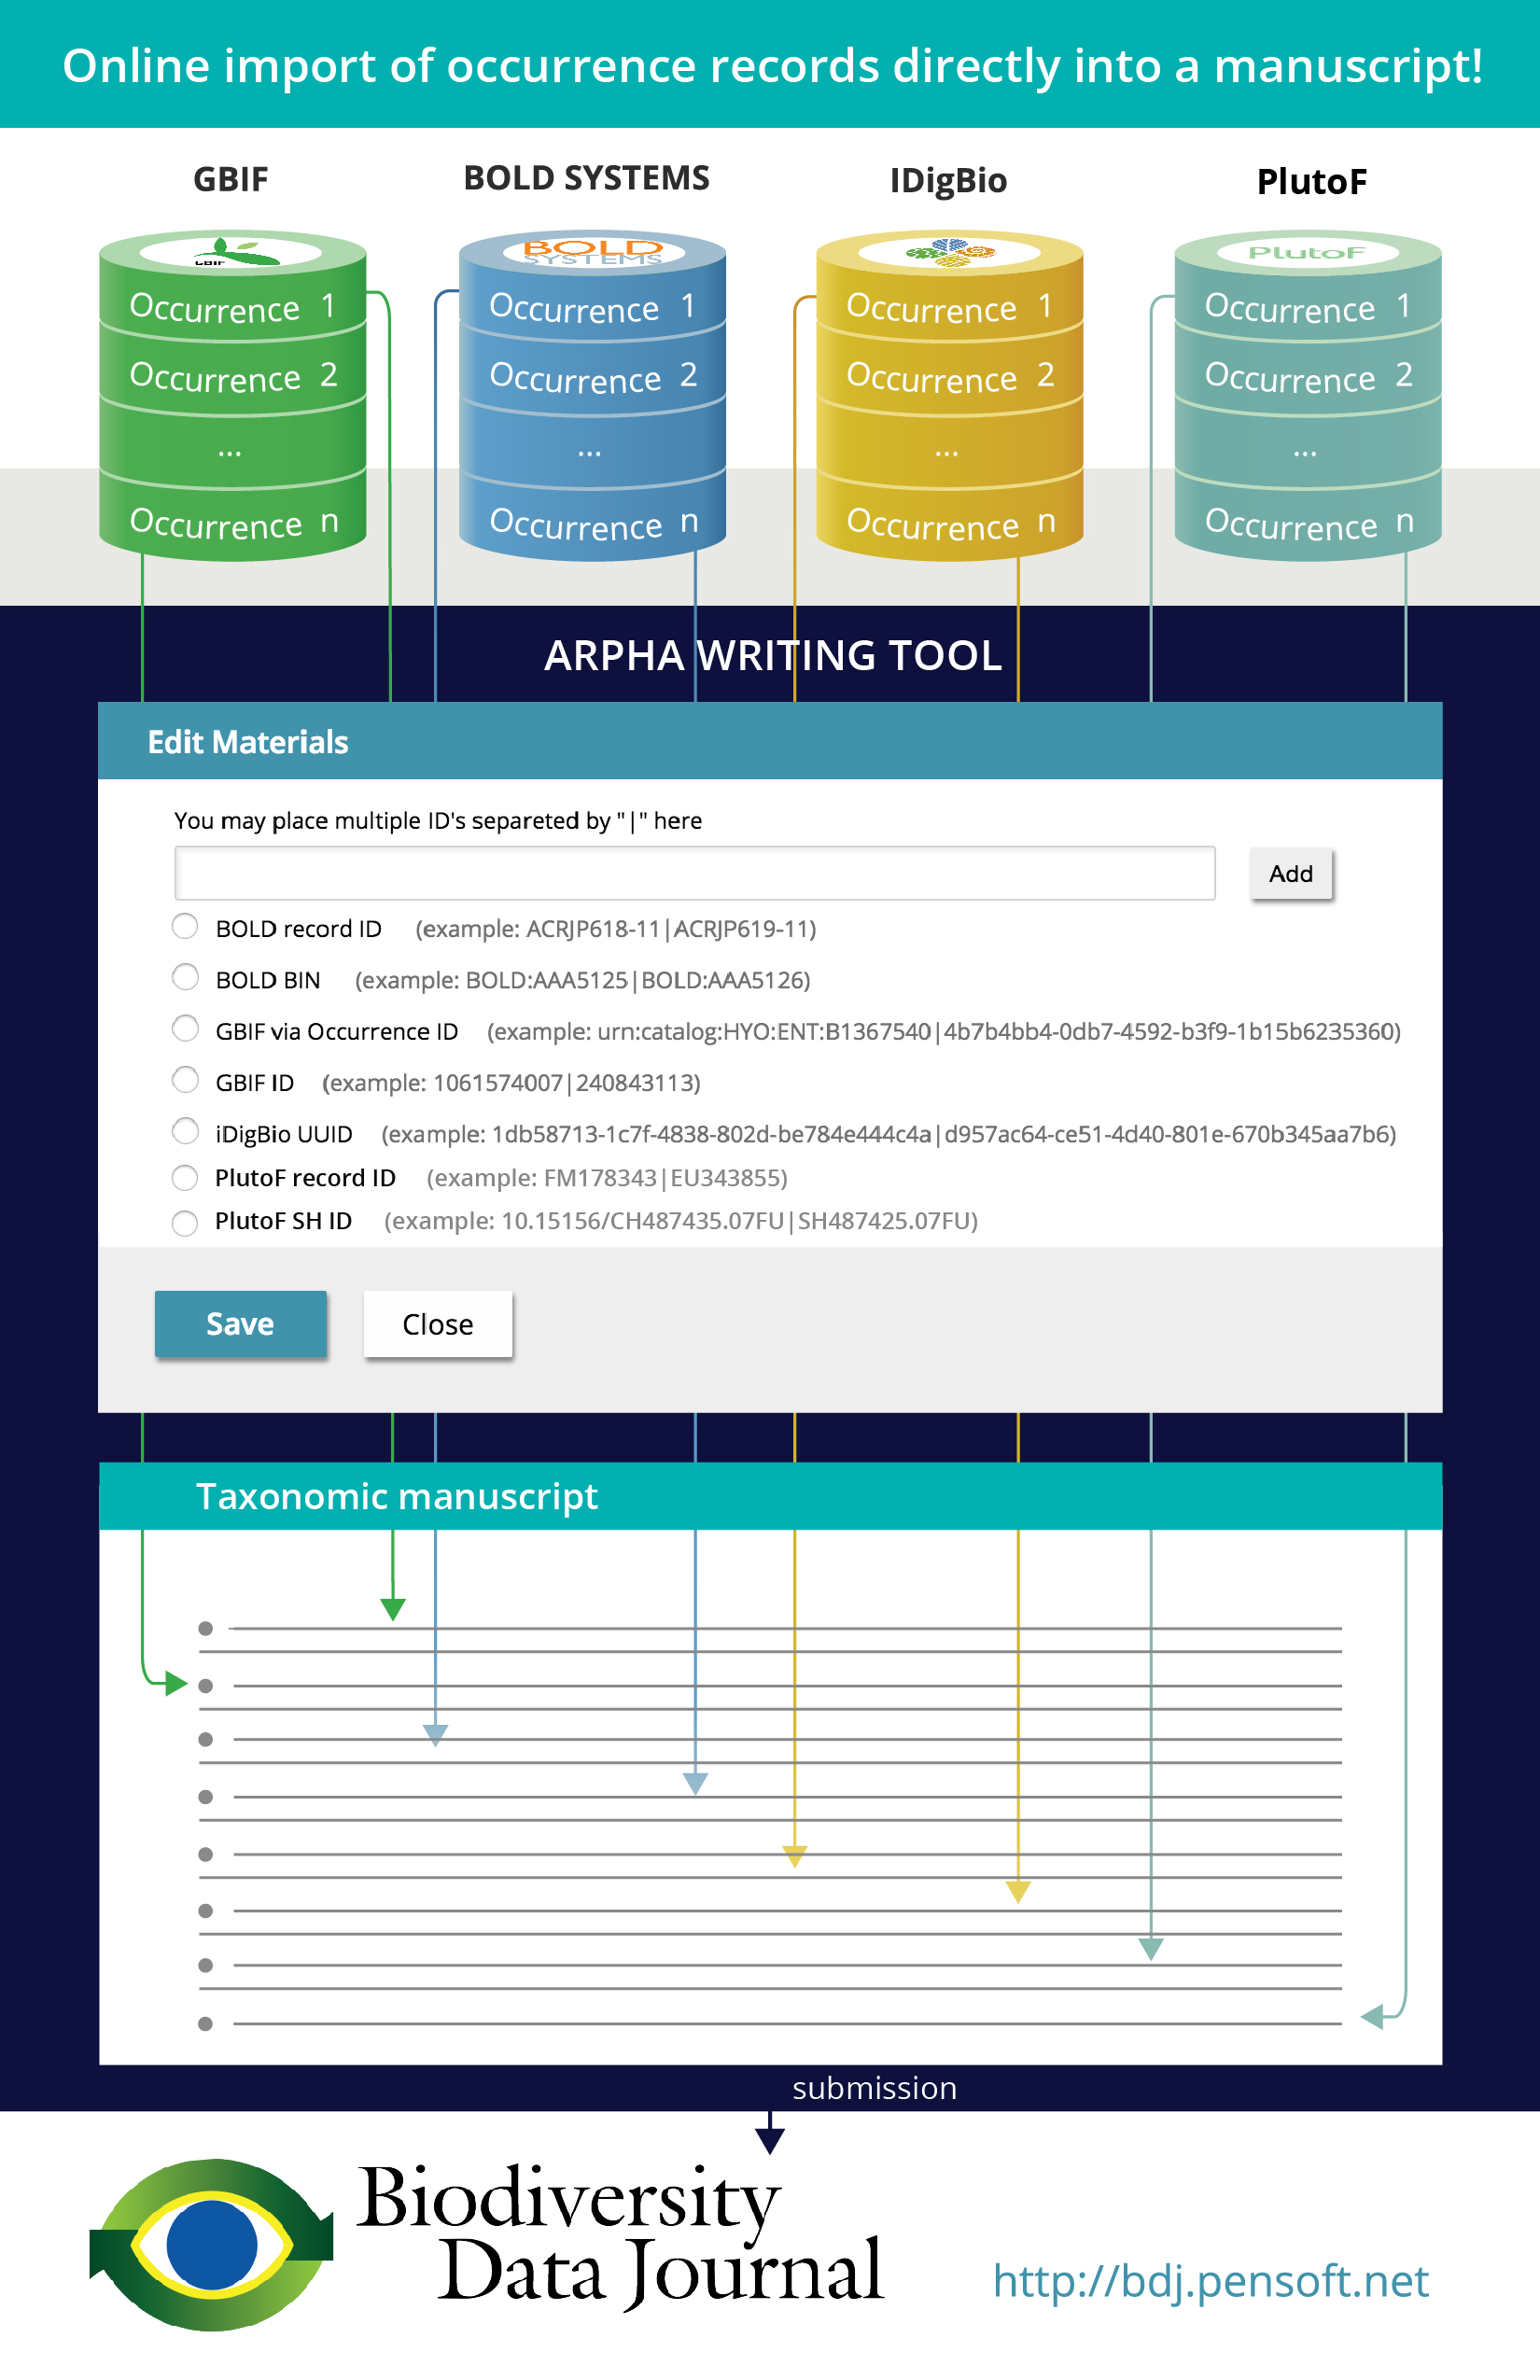
\includegraphics[width=\textwidth]{Figures/workflow-idigbio}
\decoRule
\caption{This fictionalized workflow presents the flow of information content of biodiversity specimens or biodiversity occurrences from the data portals GBIF, BOLD Systems, iDigBio, and PlutoF, through user-interface elements in AWT to textualized content in a Taxonomic Paper manuscript template intended for publication in the Biodiversity Data Journal.}
\label{fig:workflow-idigbio}
\end{figure}

\begin{figure}
\centering
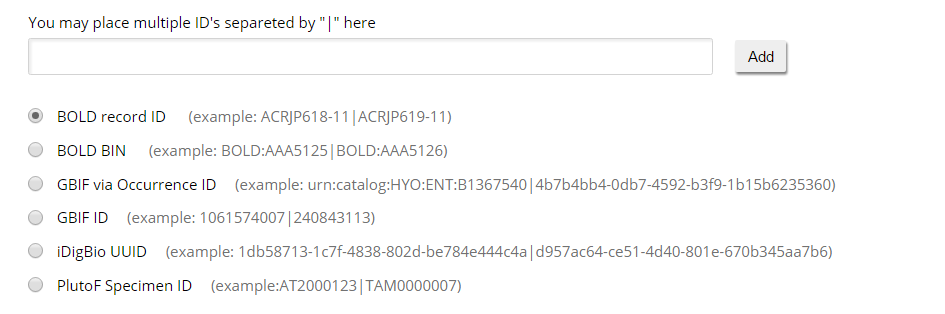
\includegraphics[width=\textwidth]{Figures/occurrence-input-mask}
\decoRule
\caption{User interface of the ARPHA Writing Tool controlling the import of specimen records from external databases.}
\label{fig:occurrence-input-mask}
\end{figure}

\subsubsection{Discussion}

We discuss the availability, or more correctly the lack of persistent unique identifiers (PID's) in the biodiversity informatics space. I furthermore discuss the challenges of importing from our different sources: GBIF, PlutoF, iDigBio, and BOLD. I emphasize how our workflow can be serve as  a curation filter for increasing the quality of specimen data via the scientific peer review process. 

\subsection{Workflow 2: Automated data paper manuscript generation from EML metadata in the ARPHA Writing Tool}

We have created a workflow that allows authors to automatically create data paper manuscripts from the metadata stored in EML (Fig.~\ref{fig:EML-download}, Fig.~\ref{fig:journal-selection}, Fig.~\ref{fig:user-interface}).

\begin{figure}
\centering
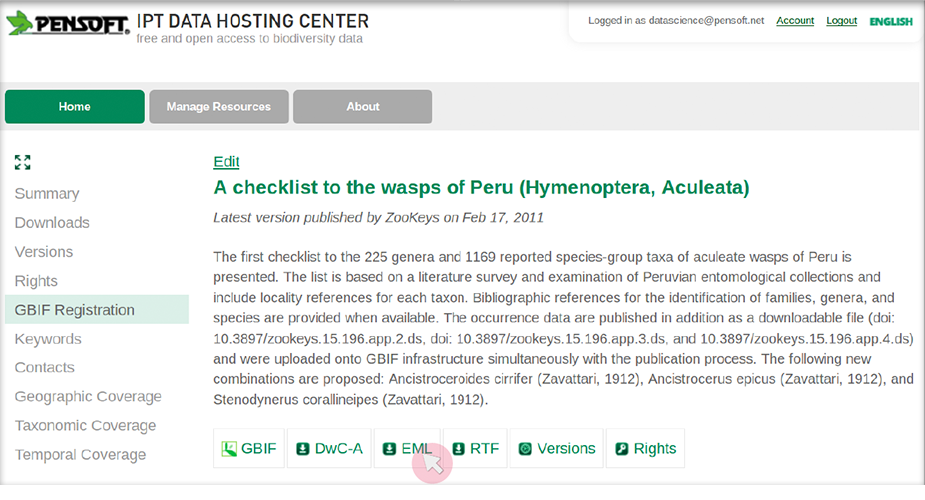
\includegraphics[width=\textwidth]{Figures/EML-download}
\decoRule
\caption{Download of an EML from the GBIF Integarted Publishuing Toolkit (IPT).}
\label{fig:EML-download}
\end{figure}

\begin{figure}
\centering
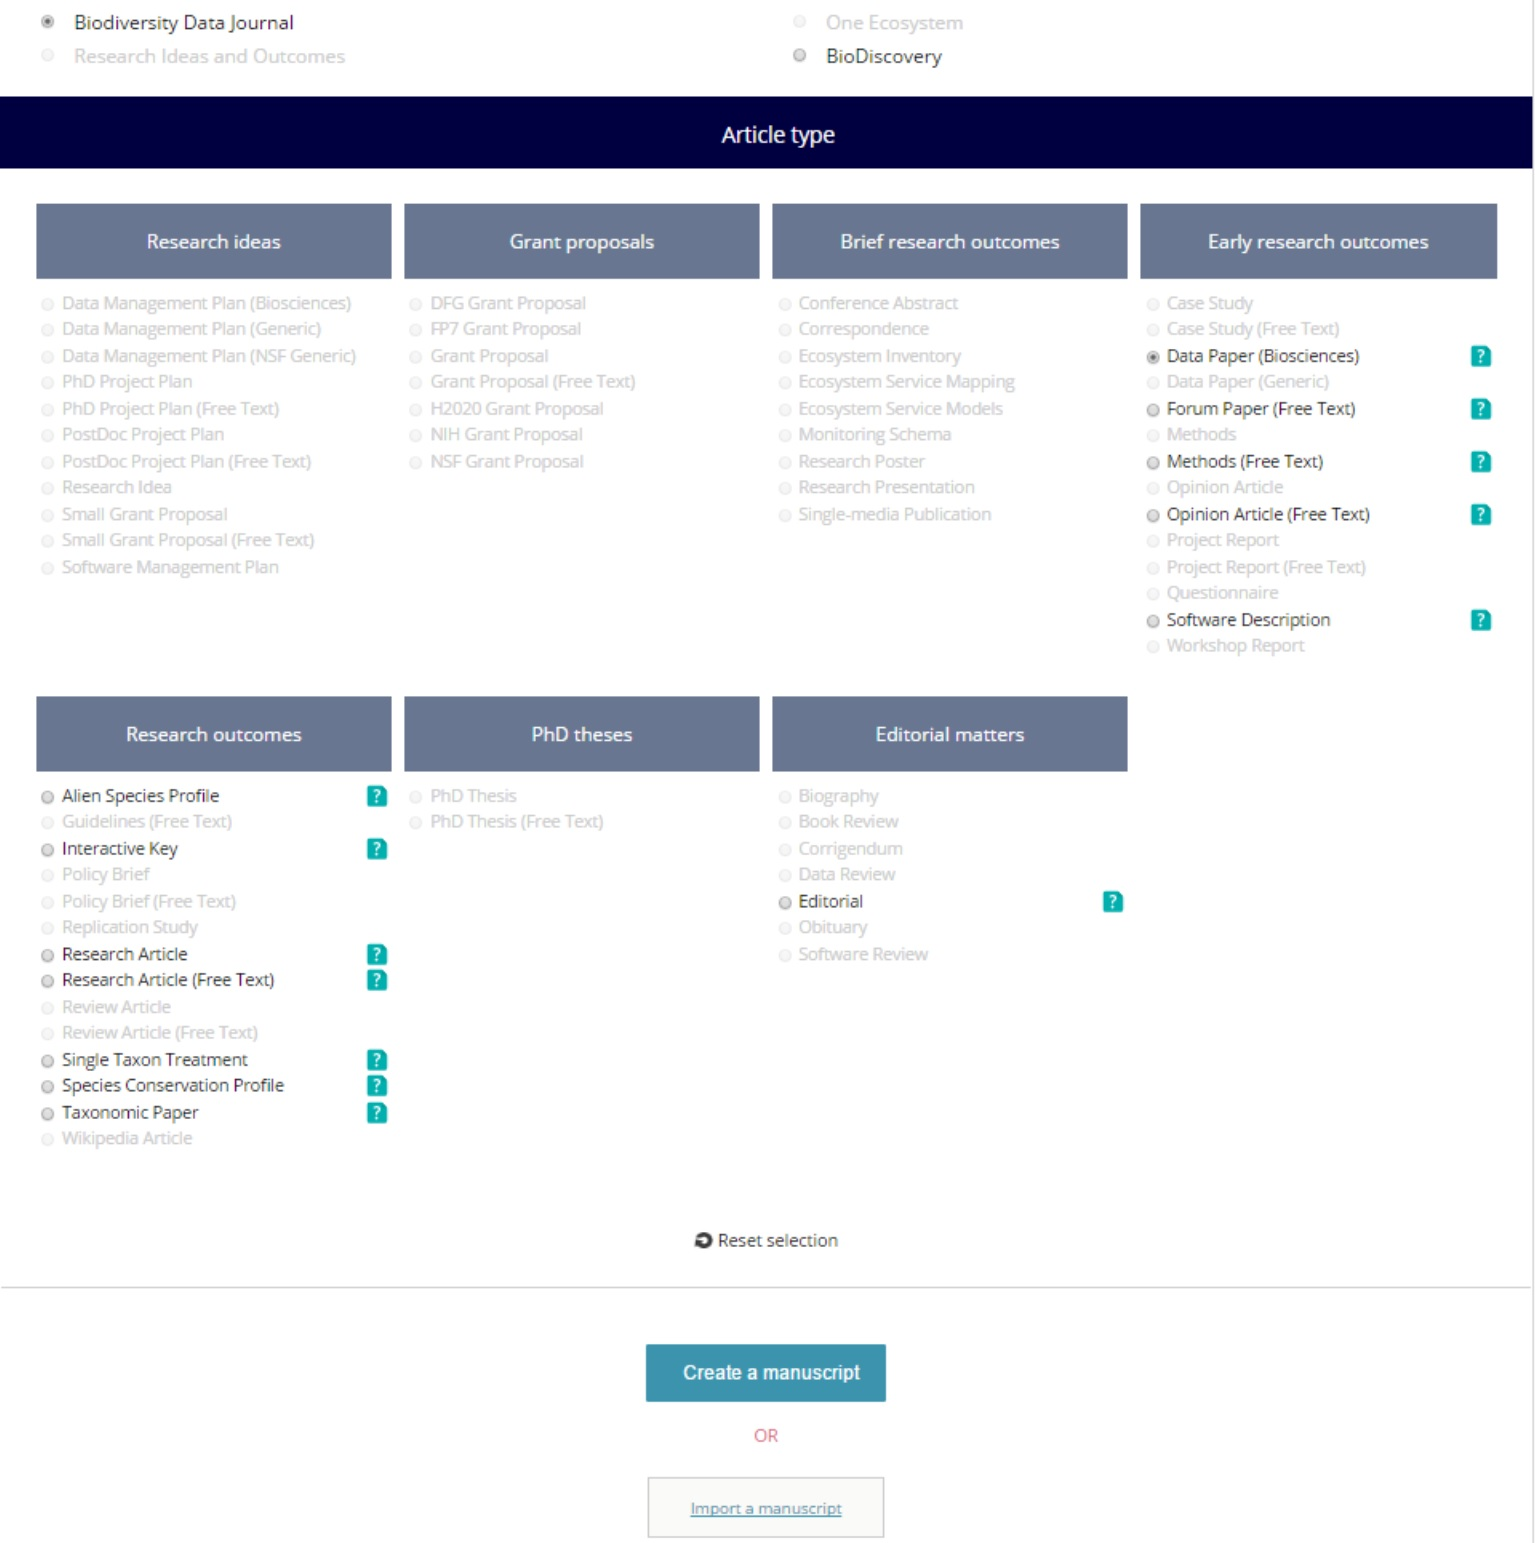
\includegraphics[width=\textwidth]{Figures/journal-selection}
\decoRule
\caption{Selection of the journal and ``Data Paper (Biosciences)'' template in the ARPHA Writing Tool.}
\label{fig:journal-selection}
\end{figure}

\begin{figure}
\centering
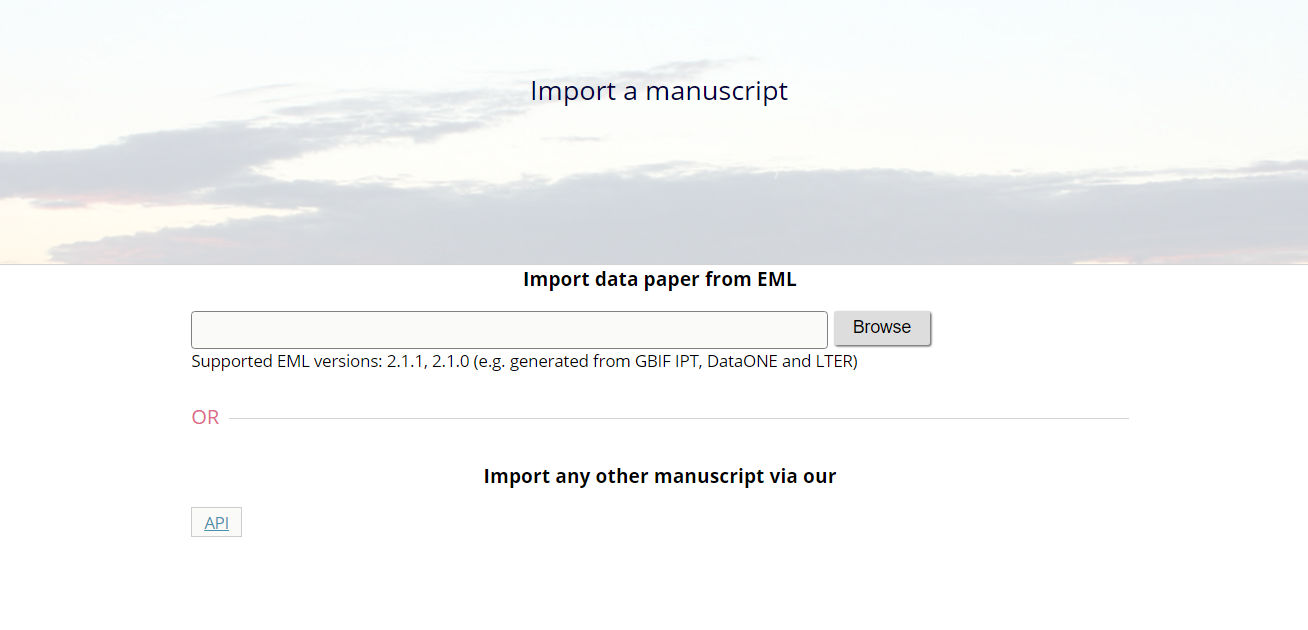
\includegraphics[width=\textwidth]{Figures/user-interface}
\decoRule
\caption{The user interface field for uploading EML files into ARPHA.}
\label{fig:user-interface}
\end{figure}

\subsubsection{Discussion}

I discuss the history of data papers and how our implementation greatly improves the availability of data papers to science practicioners. The two workflows presented generated a lively discussion at the end of the presentation, which is summarized in the Chapter.
\chapter{Резюме на глава 6: Уеб портал}
\label{chapter-webportal}

Под \href{http://openbiodiv.net}{openbiodiv.net} може да се стигне до основния портал, който дава достъп до ресурсите на OpenBiodiv. Този портал е разработен от Pensoft в подкрепа на OpenBiodiv и представя два визуални елемента на потребителя: лентата за търсене и списък с икони на приложения в долната част. Освен това, под \href {http://graph.openbiodiv.net}{{graph.openbiodiv.net}} (също достъпен от иконката SPARQL) може да се достигне работния плот OpenBiodiv за  на SPARQL.

Тези функции на потребителския интерфейс (UI) са предназначени да улеснят трите типа потребители на системата, които предвиждаме:

\begin{enumerate}
\item Основно ниво: използва лентата за търсене.
\item Ниво на специалист: използва приложения.
\item Power user: използва работната плот за SPARQL или R.
\end{enumerate}

\begin{figure}
\centering
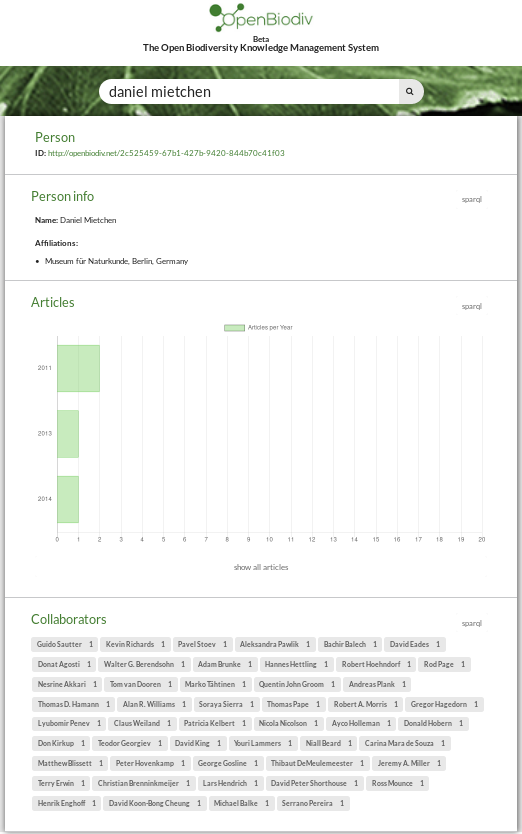
\includegraphics[width=\textwidth]{Figures/basic-level.png}
\decoRule
\caption{Илюстрация на основната употреба на OpenBiodiv за търсене на информация за човек.}
\label{fig:basic-level}
\end{figure}
%\part{Conclusion}
%\label{part:conclusion}


%----------------------------------------------------------------------------------------
%	THESIS CONTENT - APPENDICES
%----------------------------------------------------------------------------------------

\appendix % Cue to tell LaTeX that the following "chapters" are Appendices

% Include the appendices of the thesis as separate files from the Appendices folder
% Uncomment the lines as you write the Appendices

%% Appendix A

\chapter{Frequently Asked Questions} % Main appendix title

\label{AppendixA} % For referencing this appendix elsewhere, use \ref{AppendixA}

\section{How do I change the colors of links?}

The color of links can be changed to your liking using:

{\small\verb!\hypersetup{urlcolor=red}!}, or

{\small\verb!\hypersetup{citecolor=green}!}, or

{\small\verb!\hypersetup{allcolor=blue}!}.

\noindent If you want to completely hide the links, you can use:

{\small\verb!\hypersetup{allcolors=.}!}, or even better: 

{\small\verb!\hypersetup{hidelinks}!}.

\noindent If you want to have obvious links in the PDF but not the printed text, use:

{\small\verb!\hypersetup{colorlinks=false}!}.

%\include{Appendices/AppendixB}
%\include{Appendices/AppendixC}

%----------------------------------------------------------------------------------------
%	BIBLIOGRAPHY
%----------------------------------------------------------------------------------------

\printbibliography[heading=bibintoc]

%----------------------------------------------------------------------------------------

\end{document}  
